%!TEX root = ../AutoML-fuer-Segmentierung.tex
\chapter{nnUNet}
\label{ch:nnunet}


\section{Funktionsweise / Theorie}



Das nnU-Net ist ein Framework, welches sich mit der Segmentierung von medizinischen 3D-Aufnahmen mit Hilfe von automatisiertem maschinellem Lernen beschäftigt. Es wurde im Rahmen des Medical Segmentation Decathlon Wettbewerb entwickelt und gewann diesen sowie im Anschluss auch viele weitere Segmentierungs-Wettbewerbe. Die folgenden Ausführungen beruhen auf dem Paper \cite{nnunetPaper} und auf dem Paper \cite{nnunetPaperB} , beide von Fabian Isensee et al. \\
Das nnU-Net verwendet eine klassische und nicht neue U-Net Architektur (not new U-Net). Es konzentriert sich kaum auf  Architekturdesign und -suche, sondern vorrangig auf die Suche von guten Hyperparametern. Es wird eine gleiche oder sehr ähnliche U-Net Struktur immer durch eine individuell auf die individuellen Daten angepasste Trainingspipeline zur Optimierung geschickt (siehe Abbildung \ref{pic:nnUnet_Basisschema}). Das Training der Parameter des Netzes ist also individuell zugeschnitten, während die Architektur sich bei unterschiedlichen Daten nicht oder kaum unterscheidet. Es wird sich also vorrangig auf das Training des Netzes und die Suche individueller Hyperparameter für die Trainingspipeline konzentriert und nicht auf die Suche nach der Architektur. 

\begin{figure}[H]
	
	\centering
	
\includegraphics[scale=0.3]{Pictures/nnUnet/Bild01.png}
	\caption{}
	\label{pic:nnUnet_Basisschema}
\end{figure}



Das nnU-Net verwendet 3 Standardarchitekturen, welche 2D U-Net, 3D full resolution U-Net und 3D U-Net Cascade sind. Vor dem Training kann man einstellen, wie viele und welche Architekturen man trainieren möchte. Per default trainiert nnU-Net alle und wählt am Ende die beste oder die beste Kombination aus maximal zwei Architekturen aus. 2D U-Net eignet sich besonders für 2D-Daten und läuft gut auf anisotropen Daten. Es arbeitet auf den Bildern in Originalauflösung. 3D full resolution U-Net eignet sich für kleine 3D-Daten und arbeitet auch auf den Bildern in Originalauflösung. Bei größeren Bildern werden jedoch die Patches sehr klein, was zum immer größer werdenden Verlust von Kontextdaten führt. Daher gibt es das 3D U-Net Cascade für große 3D-Daten. Es besteht aus 2 hintereinander gereihten U-Nets. Das erste U-Net arbeitet auf den Bildernals ganzes, also ohne Aufteilung in Patches, in geringerer Auflösung. Diese grobe Vorsegmentierung wird zusammen mit dem Bild in Originalgröße an das zweite U-Net weitergegeben. Dieses arbeitet dann wieder auf der vollen Bildauflösung und mit Patches und erstellt eine endgültige und verfeinerte Segmentierung. Durch diesen Übergabeschritt zwischen den beiden U-Nets bleiben die Kontextdaten erhalten (siehe Abbildung \ref{pic:nnUnet_Cascade}).

\begin{figure}[H]
	
	\centering
	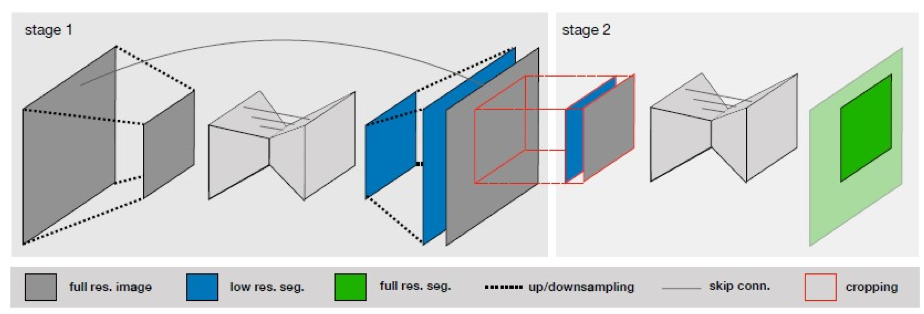
\includegraphics[scale=0.8]{Pictures/nnUnet/Bild02.png}
	\caption{nnU-Net Cascade \cite{nnunetPaper} }
	\label{pic:nnUnet_Cascade}
\end{figure}


Um die Konzentration auf die Anpassung der Hyperparameter der Trainingspipeline an den individuellen Datensatz zu erreichen, wird zunächst ein Datafingerprint aus den Eigenschaften der Trainingsdaten erstellt (siehe Abbildung \ref{pic:nnUnet_Datafingerprint}). Die hierbei genutzten Eigenschaften sind unter anderem die Imgasize, das Pixelvolumen oder die Farbkanäle, die spacing Anisotropie sowie die Anzahl der Klassen und deren Häufigkeitsverteilung. 

\begin{figure}[H]
	
	\centering
	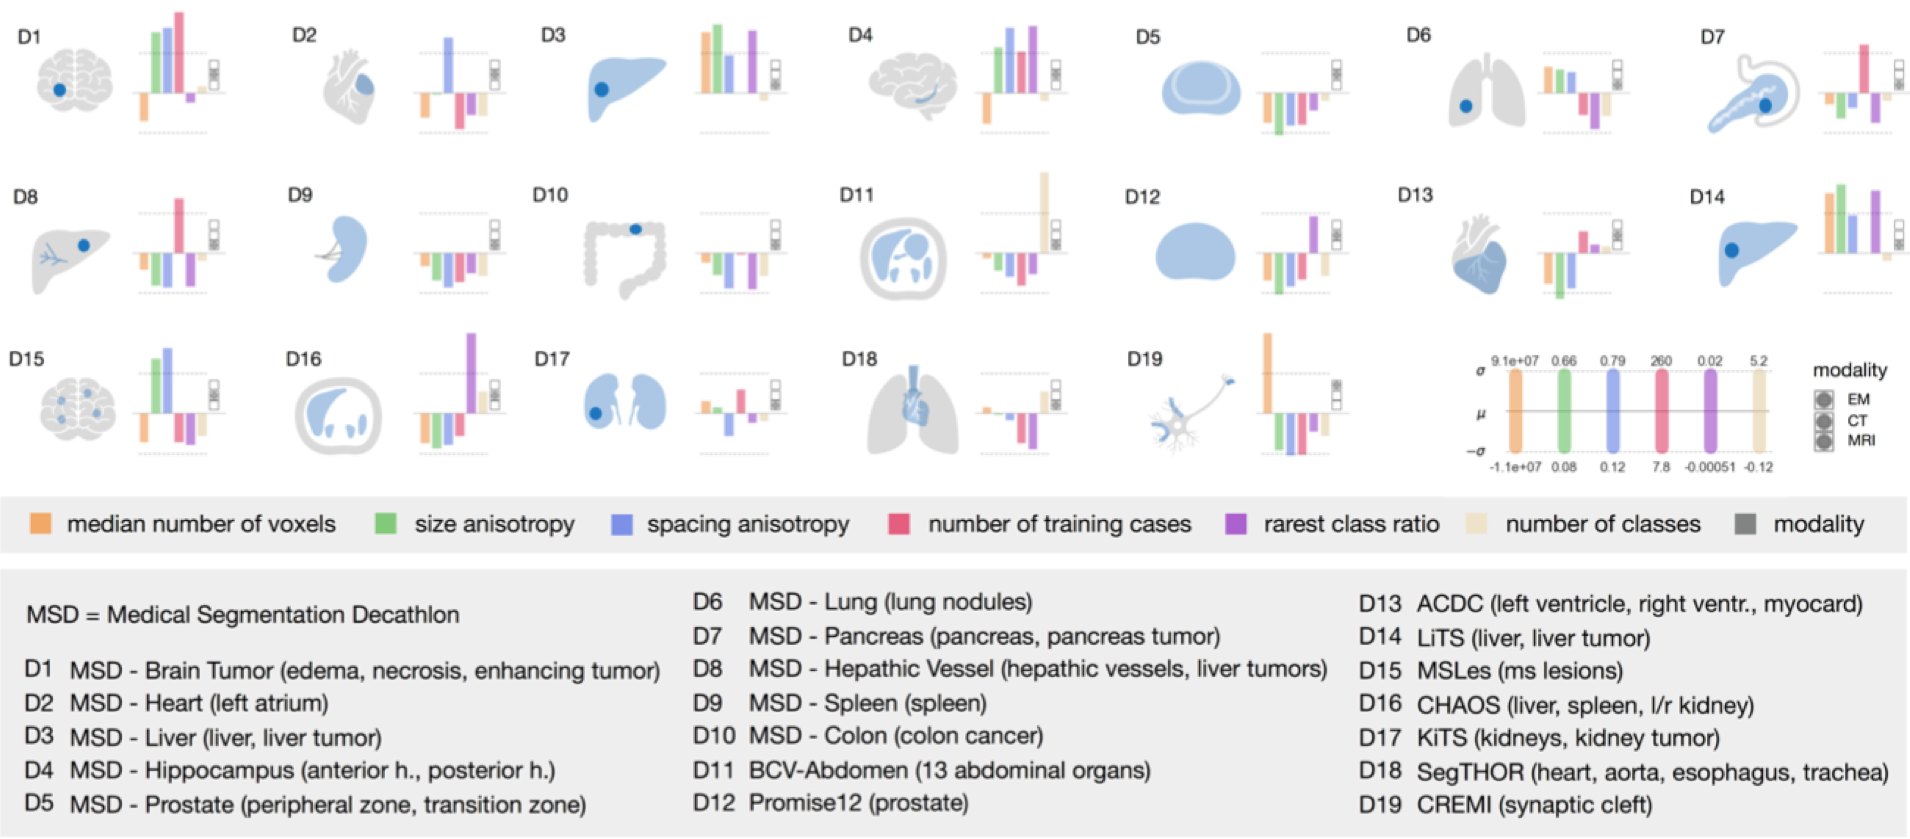
\includegraphics[scale=0.45]{Pictures/nnUnet/Bild03.png}
	\caption{Datafingerprint \cite{nnunetPaperB}}
	\label{pic:nnUnet_Datafingerprint}
\end{figure}


Aus dem Datafingerprint werden, mit Hilfe von heuristischen Regeln, die Inferred Parametern berechnet. Die Inferred Parameter umfassen die Patch Size, die Batch size, wichtige Parameter zur dynamischen Anpassung der Netzwerktopologie, wie zum Beispiel die Anzahl der Max. Poolings und Downsamplings, sowie Parameter zur Bild Vorverarbeitung. \\
Die Bestimmung der Patch size erfolgt zunächst initial über den Median der Bildgröße nach dem Resampling. Anschließend wird mit dieser Patch Size die Architektur konfiguriert und geschaut ob ausreichend GPU-Memory zur Verfügung steht. Steht nicht ausreichend GPU-Memory zur Verfügung, so wird die Patch Size reduziert und die Architektur darauf aufbauend neu konfiguriert. Dies wird so oft wiederholt, bis ausreichend GPU-Memory verfügbar ist. Anschließend wird die Batch Size angepasst und das Netzwerk abschließend konfiguriert (Siehe Abbildung \ref{pic:nnUnet_PatchSize}). Dabei muss beachtet werden, dass die Patch Size immer durch $2^i$ teilbar sein muss (mit i = Anzahl an Downsampling Operationen) da sich die Patch Size pro Downsampling Operation halbiert. Ist das nicht gegeben, so wird die Patch-Size entsprechend vergrößert oder verkleinert bis sie in allen Dimensionen durch $2^i$ teilbar ist.
 
 \begin{figure}[H]
 	
 	\centering
 	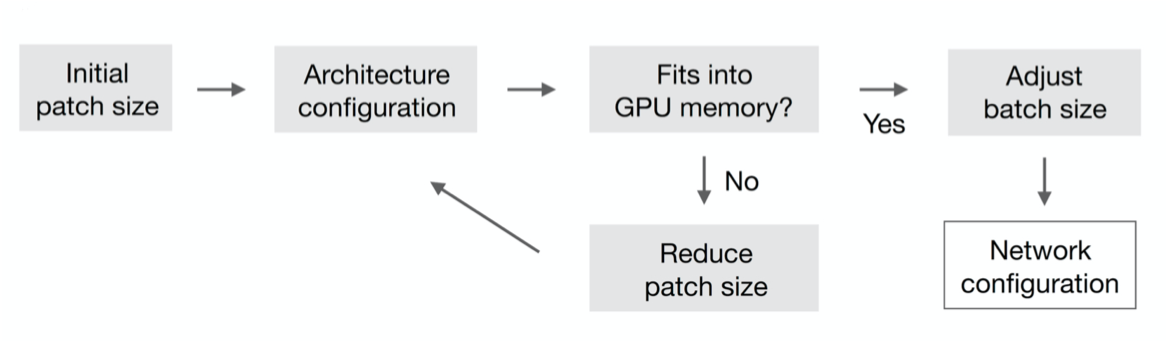
\includegraphics[scale=0.6]{Pictures/nnUnet/Bild04.png}
 	\caption{Patch Size Ermittlung \cite{nnunetPaperB} }
 	\label{pic:nnUnet_PatchSize}
 \end{figure}
 

Im Anschluss an die Inferred Parameter wird der Pipelinefingerprint erstellt, welcher sich aus den Inferred Parametern, den Blueprint Parametern und den empirischen Parametern zusammensetzt. Während die bereits beschriebenen Inferred Parameter für die entscheidende Anpassung an einen neuen Datensatz sorgen, sind die Blueprint Parameter unabhängig von dem Datensatz. Sie enthalten die drei möglichen Architekturen, sowie Hyperparameter mit festen default Werten, wie Verlustfunktion, Training Schedule, Data Augmentation, Normalisierung, stochastic Gradient oder  Aktivierungsfunktion (siehe Abbildung \ref{pic:nnUnet_Pipelinefingerprint}). Die Verlustfunktion wird als die Summe von Dice-Verlustfunktion und Cross-Entropy-Verlustfunktion gewählt. Dies wird gemacht, da medizinische Bilddaten oft Probleme mit einer großen Disbalance im Vorkommen der einzelnen Klassen haben und darum im Training seltener vorkommende Klassen unterepräsentiert sind und gleichzeitig durch die Lösung dieses Problems die Verteilung der Klassen verzerrt wird. An der Zusammensetzung dieser beiden Verlustfunktionen könnte man also auch arbeiten, wenn man das Framework auf andere Arten von Datensätzen anpassen wollte. Das Training läuft über 1000 Epochen mit jeweils 250 Trainingsiterationen. 

\begin{figure}[H]
	
	\centering
	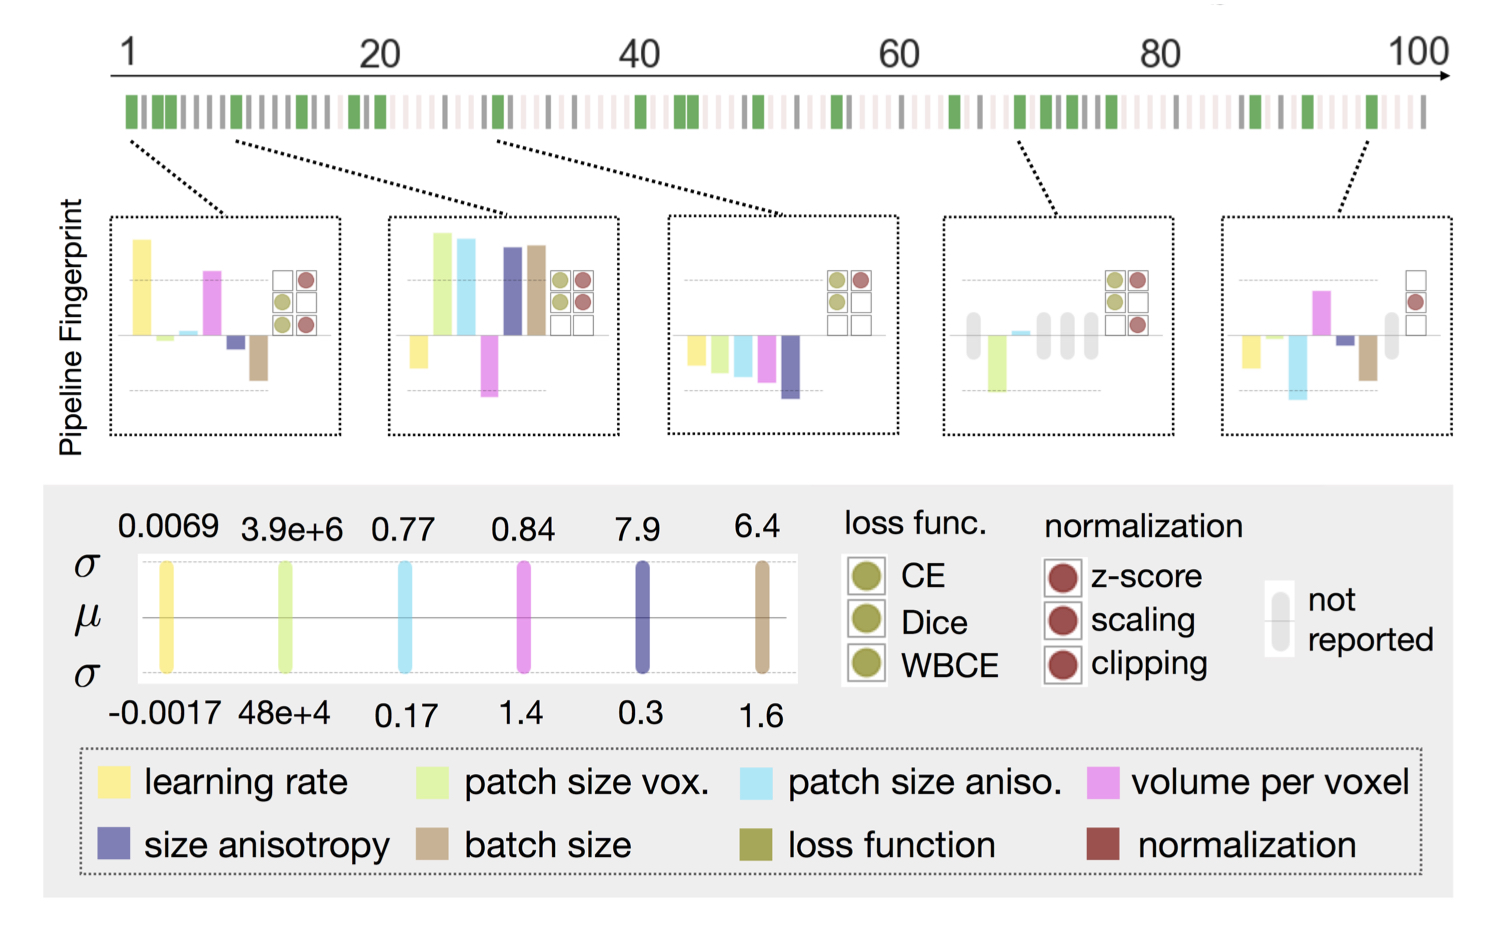
\includegraphics[scale=0.5]{Pictures/nnUnet/Bild05.png}
	\caption{Pipelinefingerprint \cite{nnunetPaperB} }
	\label{pic:nnUnet_Pipelinefingerprint}
\end{figure}

Da die empirischen Parameter nicht direkt aus dem Datensatz erschlossen werden können, werden sich nach dem Training empirisch bestimmt. Sie werden zur Nachbearbeitung und bei der Auswahl der besten Netzstruktur genutzt. 


\section{Unsere Arbeit / Praxis}
\begin{figure}[H]
\begin{tabular}{|c|c|c|c|c|c|}
\hline 
\multirow{3}{*}{\textbf{Datensatz}} &  &  & & Train-& Test- \\ 
 & \textbf{Split} & verwendete & \textbf{Trainingszeit} & \textbf{Accuracy}& \textbf{Accuracy} \\ 
 & (Train:Test) & \textbf{nnUNet-Variante} & (h) & (Dice)& (Dice)  \\ 
\hline 
\hline
Larven \cite{larven} & 265:0 $\approx$ 1:0 & 2D & 8:30 & 0.99970 & - \\ 
\hline 
Larven \cite{larven}& 173:92 $\approx$ 2:1 & 2D & 6:45 & 0.99982 & 0.94459 \\ 
\hline 
Pascal VOC12 \cite{PascalVOCDatensatz}& 2516:340 $\approx$ 7:1 & 2D & 26:00 & 0.90266 & 0.34953 \\ 
\hline 
Retina-2D \cite{retina2d} (manuelle & \multirow{2}{*}{56:34 $\approx$ 2:1} & \multirow{2}{*}{2D} & \multirow{2}{*}{23:20} & \multirow{2}{*}{0.99977} &\multirow{2}{*}{0.93606}  \\ 
Data-Augmentation)&  & & & &  \\ 
\hline 
Retina-2D \cite{retina2d} (minimal) & 13:32 $\approx$ 1:2 & 2D & 21:15 & 0.99999 &  0.83013 \\ 
\hline 
\multirow{2}{*}{CT \cite{ctDatensatz} (2000 Epochen)} & \multirow{2}{*}{19:0 $\approx$ 1:0} & 3D\_fullres & \multirow{2}{*}{$\approx$ 86:00}  & \multirow{2}{*}{0.67197} & \multirow{2}{*}{-} \\ 
 &  & (\textbf{2000} Epochen) & &  &  \\ 
\hline 
CT \cite{ctDatensatz} & 19:0 $\approx$ 1:0 & 2D & 29:00 & 0.00109 & - \\ 
\hline 
\multirow{2}{*}{CT \cite{ctDatensatz}} & \multirow{2}{*}{19:0 $\approx$ 1:0} & \multirow{2}{*}{3D\_cascade} & $\approx$ 39:00 + 48:00 & \multirow{2}{*}{0.20865} & \multirow{2}{*}{-} \\ 
 &  &  & =87:00 &  & \\ 
\hline 
Retina-3D \cite{retina3dDatensatz} & 14:7 $\approx$ 2:1 & 3D\_fullres & 45:15 & 0.91863 & 0.83759 \\ 
\hline 
Retina-3D \cite{retina3dDatensatz} & 14:7 $\approx$ 2:1  & 2D & 19:00 & 0.98574 & 0.78931 \\ 
\hline 
Retina-3D \cite{retina3dDatensatz} (Ensemble) & 14:7 $\approx$ 2:1 & 2D \& 3D\_fullres & - & 0.97775 & 0.82363 \\ 
\hline
\end{tabular} 
\caption{Datensätze, auf denen wir trainiert haben (jeweils 1000 Epochen auf GPUv100)}
\label{tab:Training}
\end{figure}

Grundsätzlich haben wir für jeden folgenden Datensatz die Ursprungsdateien in Nifti-Dateien umgewandelt und meistens zufällig in einen Train- und Testsplit aufgeteilt, außer bei dem 3D-CT Datensatz, da wird dort auch mit allen Samples im Trainsplit keine sonderlich guten Ergebnisse erzielen konnten, und dem ersten Versuch auf dem Larvendatensatz.\\
Der generelle Arbeitsablauf bestand bei uns aus der Befehlsabfolge:
\begin{lstlisting}[language=bash]
nnUNet_plan_and_preprocess -t <TASK-ID> --verify_dataset_integrity
\end{lstlisting}
bzw. für 2D-Datensätze, da dort kein 3D-Modell anwendbar ist:
\begin{lstlisting}[language=bash]
nnUNet_plan_and_preprocess -t <TASK-ID> -pl3d None
\end{lstlisting}
Dieser Befehl bereitet das Training vor und prüft, ob der gegebene Datensatz als Nifti-Dateien korrekt ist, indem Wertebereiche und das Vorhandensein aller Dateien geprüft wird. Da dieser Befehl das Training vorbereitet, muss er mit den gleichen verfügbaren Ressourcen wie auch später das Training aufgerufen werden, in unserem Fall auf dem GPUv100 Knoten von Palma II.\\\\
Danach kann das Training für die einzelnen Netzvarianten (2d, 3d\_fullres, 3d\_cascade gestartet werden:
\begin{lstlisting}[language=bash]
# 2d
nnUNet_train 2d nnUNetTrainerV2 <TASK-ID> all --npz
# 3d_fullres
nnUNet_train 3d_fullres nnUNetTrainerV2 <TASK-ID> all --npz
# Cascade
nnUNet_train 3d_lowres nnUNetTrainerV2 <TASK-ID> all --npz
nnUNet_train 3d_cascade_fullres nnUNetTrainerV2CascadeFullRes
	 <TASK-ID> all --npz
\end{lstlisting}
Dabei verwenden wir für 3D-Datensätze immer 3d\_fullres und die 2d-Variante, für 2D-Datensätze immer nur die 2d Variante. Falls das Framework es für einen 3D-Datensatz notwendig hält bzw. überhaupt zulässt, wird auch 3d\_cascade verwendet.
Der Parameter --npz sorgt dafür, dass die Softmax-Ausgaben zusätzlich gespeichert werden, was zwar sehr viel Festplattenspeicher benötigt, uns aber später ein eventuelles Ensembling der Predictions ermöglicht.\\
Der Parameter \enquote{all} gibt an, welcher der 5 Folds, die das Framework automatisch erstellt, zur Validierung benutzt wird, während die anderen 4 dem Training dienen.
Der Autor des Frameworks vermutet, dass wenn man statt \enquote{all} alle Werte 0 bis 4 verwendet und hinterher aus den 5 verschiedenen Folds ein Ensemble bildet die finale Performance besser ist im Vergleich zu \enquote{all}, jedoch hat auch er keine empirischen Beweise dafür \cite{nnunetGithub-Folds}. Wir haben uns für \enquote{all} entschieden, da die Handhabung dann etwas einfacher wird und wir vermuten, dass die zum Training benötigte Zeit deutlich geringer ist, da lediglich ein Modell aus allen Trainingsdaten trainiert wird, und nicht 5 verschiedene basierend auf einer verschiedener Aufteilung der Folds. Außerdem sind unsere Ergebnisse trotz der nicht optimalen Wahl der Parameter ziemlich gut (s. Tabelle \ref{tab:Training}). \\
Nach dem Beenden des Trainings lassen wir uns von dem Framework die Predictions zu dem Train- und Testsplit erzeugen:
\begin{lstlisting}[language=bash]
nnUNet_predict -i <Pfad zu Original-Niftis> -o <Prediction-Pfad>
 -m <2d, 3d_fullres oder 3d_cascade_fullres> -t <TASK-ID> -f all -z
\end{lstlisting}
Der Parameter -z sorgt auch hier wieder für das Speichern der Softmax-Werte, um später eventuell ein Ensembling aus verschiedenen Netzvarianten zu bilden.\\\\
Abschließend erstellen wir mit dem Framework eine Auswertung der Performance auf dem Datensatz, indem wir für den Train- und Testsplit die Ground-Truth Segmentierung mit den Predictions vergleichen:
\begin{lstlisting}[language=bash]
nnUNet_evaluate_folder -ref <Ground-Truth-Pfad>
 -pred <Prediction-Pfad> -l <Klassennummern>
\end{lstlisting}
<Klassennummern> ist hierbei eine Liste aller Klassennummern, die in der Auswertung berücksichtigt werden. Da uns die Performance auf dem Hintergrund (0) nicht interessiert, starten wir bei 1 und gehen z.B. bei Pascal VOC12 \cite{PascalVOCDatensatz} alle Klassen durch \textit{-l 1 2 3 4 ... 20}. Die erzeugt in dem Ordner, in dem die Predictions liegen eine JSON-Datei mit ausführlichen Informationen über die Güte der Predictions je Sample und je vorhandener Klasse, aus der wir einen Scatterplot erstellen.



% Aufteilung in 2D/3D erstmal weggemacht, ich gehe chronologisch durch

\subsection{Datensätze aus dem Paper}
Nach unseren schlechten vorherigen Erfahrungen mit (Auto-) Deeplab \cite{deeplabGithub} und insbesondere NAS-Unet \cite{nasunetGithub} haben wir zuerst versucht die bemerkenswert guten Ergebnisse \parencite[Kapitel 4, Table 2]{nnunetPaper} auf den Datensätzen der Medical Segmentation Decathlon Challenge \cite{msdChallenge} mit dem Framework zu reproduzieren. Wir haben die 3D-Datensätze Spleen, Lung und Heart \cite{msdChallenge} ausprobiert und konnten auf allen ähnliche Ergebnisse wie im Paper \cite{nnunetPaper} erzielen.\\

\subsection{Larven-Datensatz}
\subsubsection{Larven-Datensatz ohne Testsplit}
\begin{figure}[H]
\centering
\includesvg[height=6.5cm]{Pictures/nnUnet/Praxis/Task200-Larven-nur-train/Haeufigkeitsverteilung-200-Larven-Train}
\caption{Anteil von Objekt (Larve) je Sample im Trainsplit (alle 265 Samples) mit Durchschnitt $\approx$ 5,8\%}
\label{pic:Haeuf_200}
\end{figure}
Nachdem wir die Ergebnisse im Paper erfolgreich reproduzieren konnten haben wir versucht einen eigenen Datensatz in das Framework zu geben. Dabei ist zu erwähnen, dass unser Larven-Datensatz \cite{larven} ein 2D Datensatz ist. Er beinhaltet Graustufen-Bilder von Larven auf einer Glasscheibe, die mittels Frustrated Total Internal Reflection abgelichtet wurden. Ziel ist es, die Larven zu segmentieren und die Verschmutzungen um die Larven herum dabei zu ignorieren. Jedoch ist nnUNet nicht dafür entworfen worden auf 2D-Datensätze angewendet zu werden, besonders wenn die Datensätze aus der \enquote{non-biomedical domain} \cite{nnunetGithub2D-Daten} stammen.\\
Dies ist jedoch nicht als Einschränkung des Funktionsumfangs zu verstehen, sondern lediglich als Vorwarnung, dass die Ergebnisse eventuell nicht gut ausfallen werden.\\\\
Wir haben das zum Framework gehörige Python-Script \cite{nnunetGithub2D-Pythonscript} nur leicht modifizieren müssen und konnten den 2D Datensatz in Nifti-Dateien (.nii.gz) konvertieren und so in das Framework geben.\\
Da es sich hierbei um unseren ersten Test des Frameworks mit eigenem Datensatz handelte haben wir zuerst keinen Test-Split vorgesehen und alle 265 Bilder als Trainingsdaten benutzt.
\begin{figure}[H]
\centering
\begin{minipage}{.6\textwidth}
\begin{subfigure}{\textwidth}
\centering
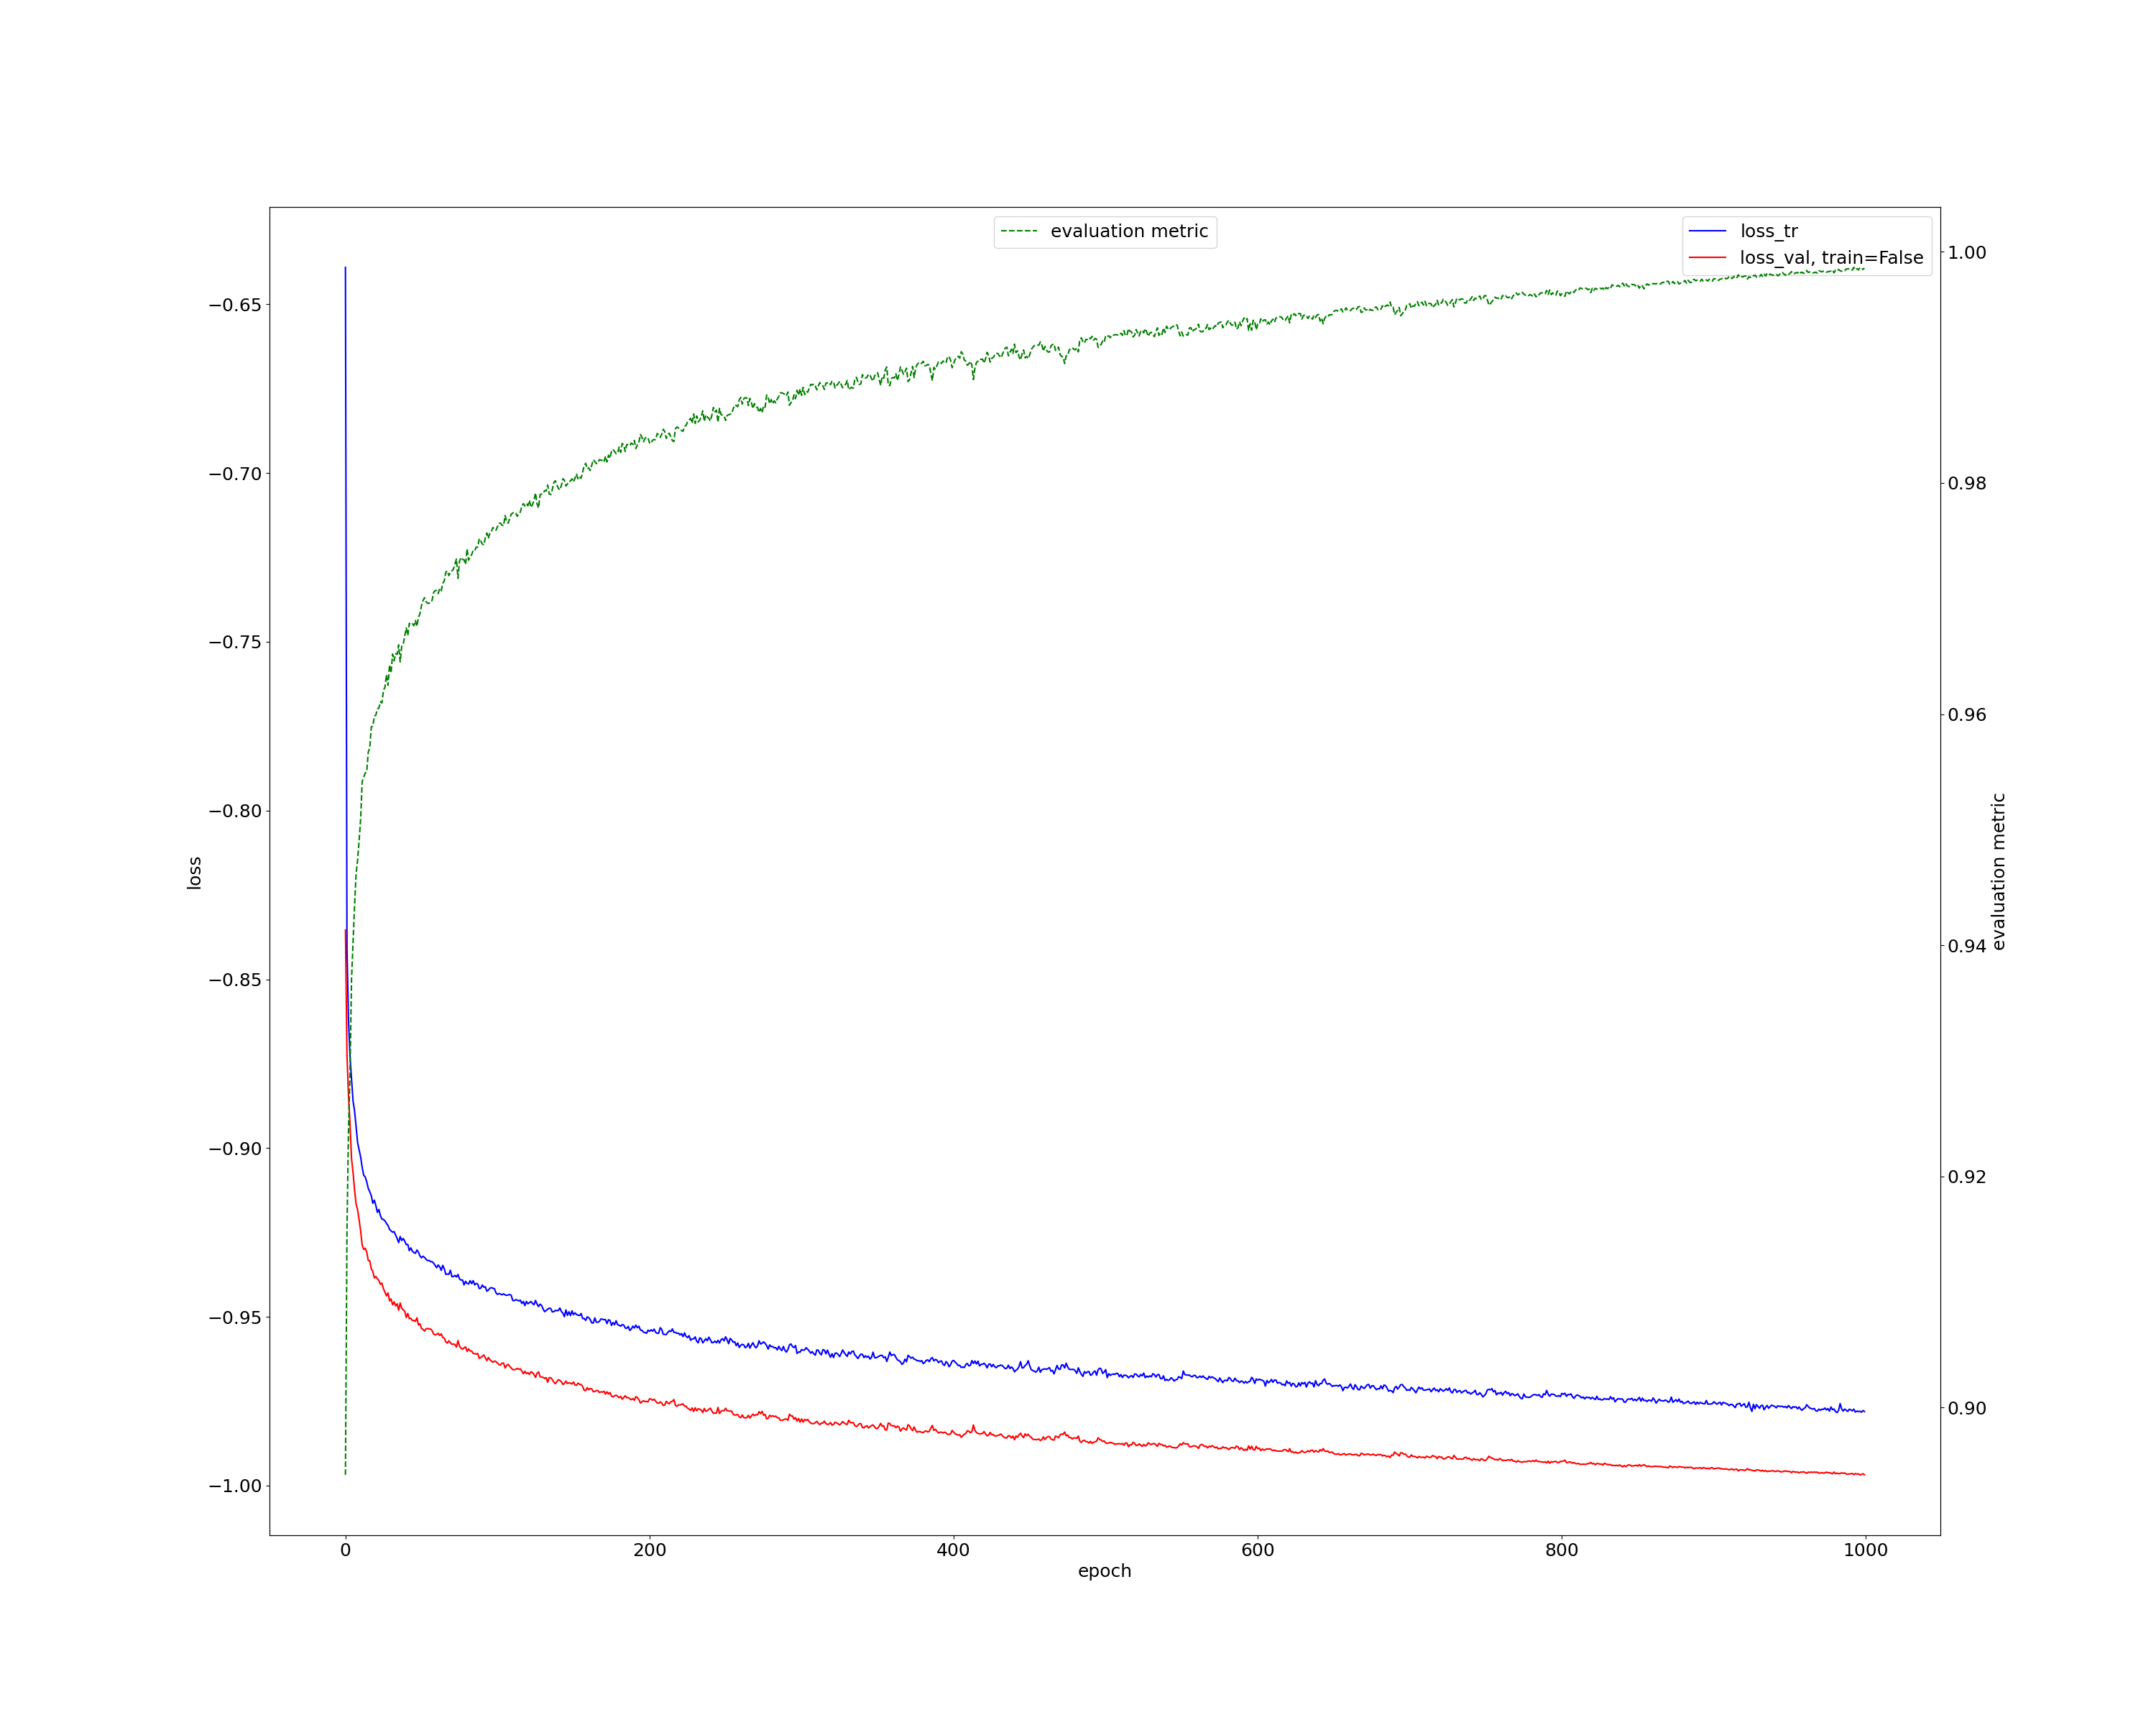
\includegraphics[width=\textwidth]{Pictures/nnUnet/Praxis/Task200-Larven-nur-train/progress_200-Larven-nur-train.png}
\caption{Verlauf des Dice-Koeffizienten beim Training über 1000 Epochen}
\label{pic:Prog_200}
\end{subfigure}
\end{minipage}%
\begin{minipage}{.4\textwidth}
\begin{subfigure}{\textwidth}
\includesvg[width=\textwidth]{Pictures/nnUnet/Praxis/Task200-Larven-nur-train/Scatterplot-Dice-200-Larven-Train}
\caption{Scatterplot der Dice-Koeffizienten je Sample (265 Stück)}
\label{pic:Dice_200}

\end{subfigure}
\end{minipage}
\caption{Dice-Koeffizienten auf dem Trainsplit zum Larvendatensatz ohne Testsplit}
\end{figure}

\begin{figure}[H]
\centering
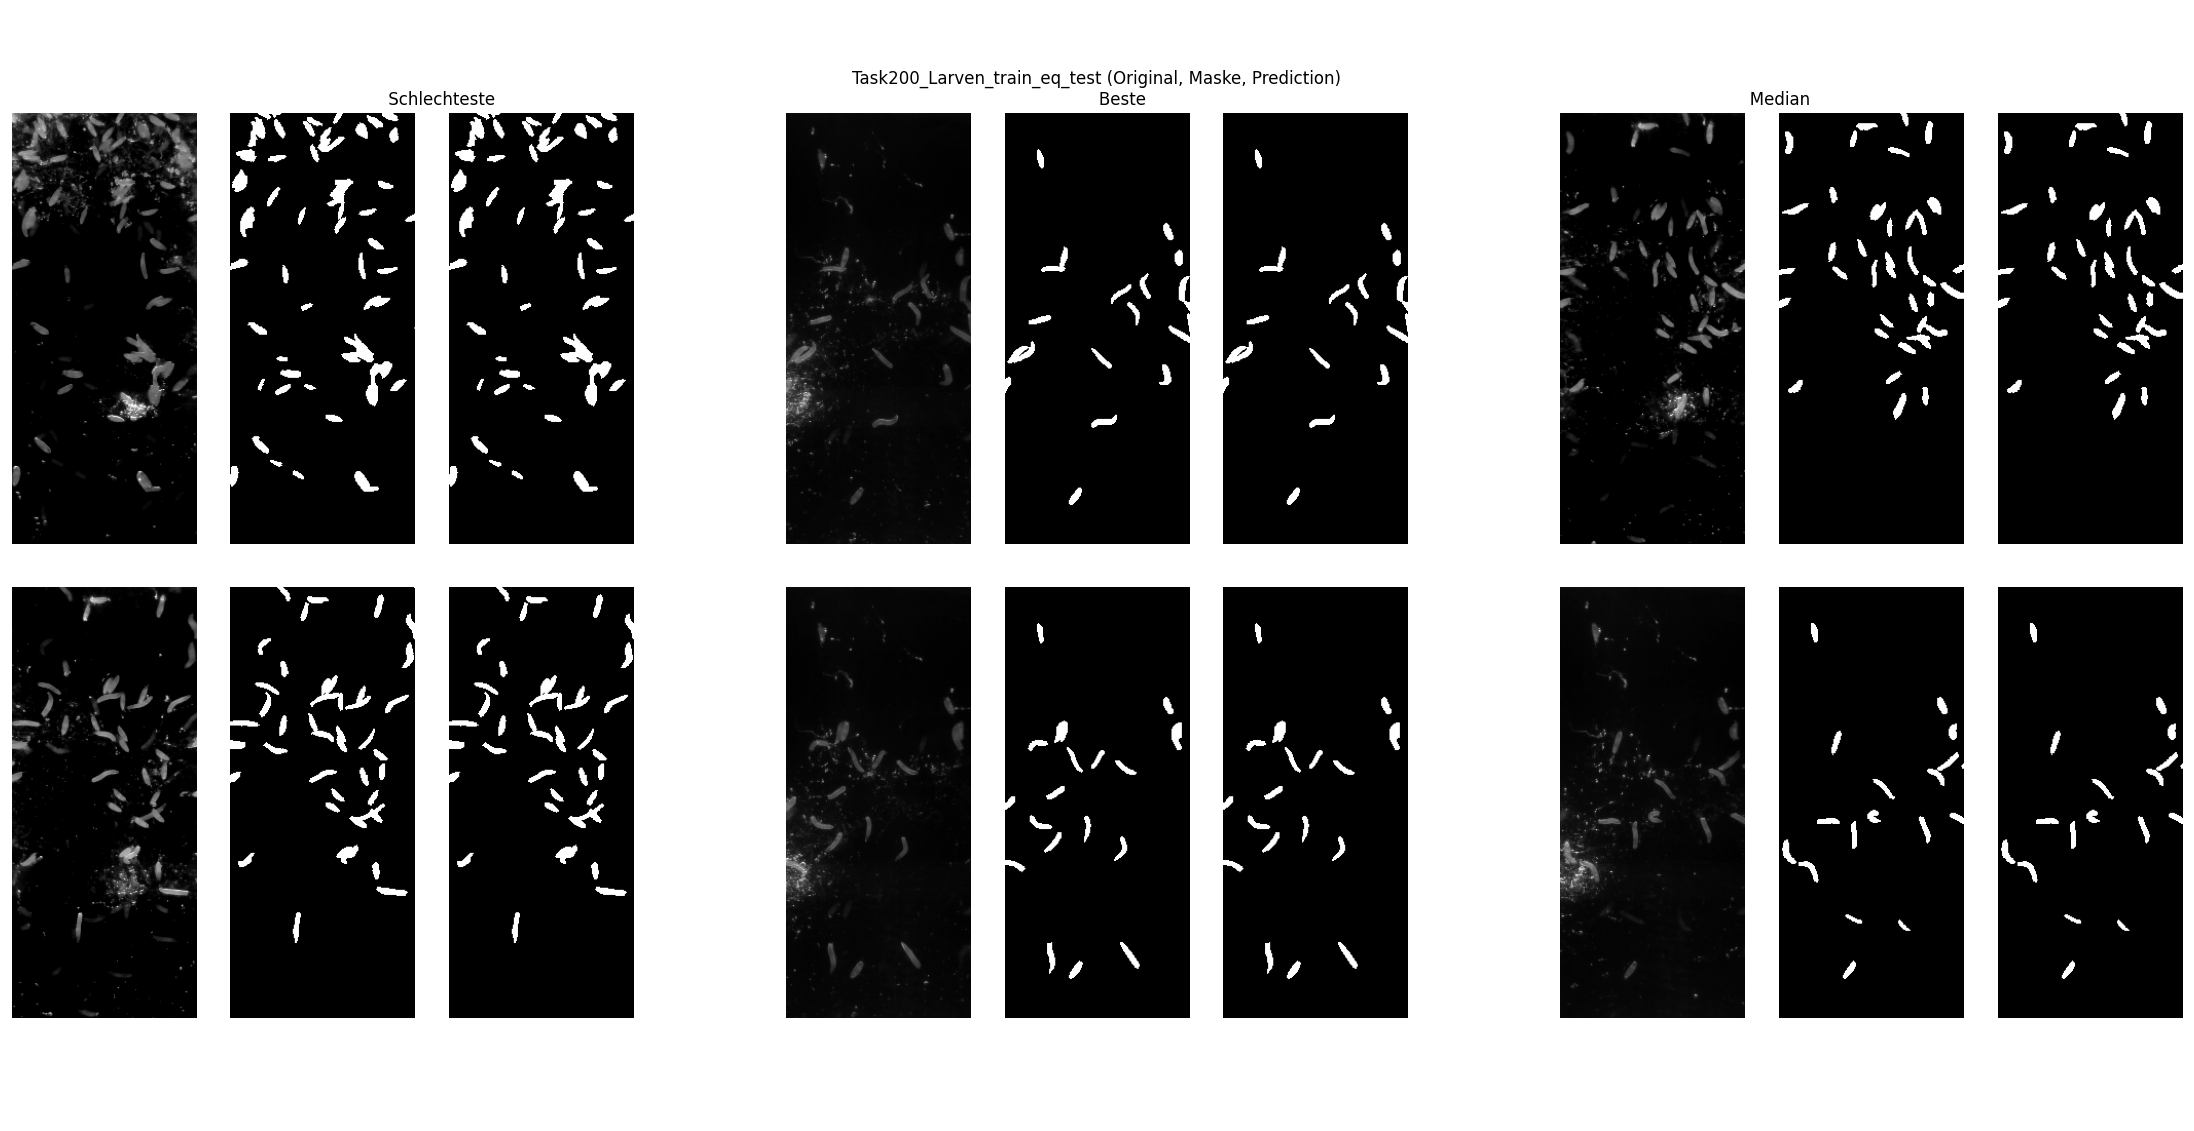
\includegraphics[height=0.35\textheight, width=\textwidth]{Pictures/nnUnet/Praxis/Task200-Larven-nur-train/Vis-Train.png}
\caption{Visualisierung des Trainsplits auf dem Larvendatensatz ohne Testsplit (links: schlechteste Ergebnisse, mitte: beste Ergebnisse, rechts: Ergebnisse im Median; jeweils Original, Ground-Truth und Prediction)}
\label{pic:Vis-Train_200}

\end{figure}
Wir konnten bei unserem ersten Versuch einen eigenen Datensatz in das Framework zu geben einen Dice-Wert von durchschnittlich $> 0.999$ erzielen und auch die am schlechtesten segmentierten Samples liegen weit über $0.99$, wie in Abbildung \ref{pic:Dice_200} zu erkennen ist.
Auch bei der Visualisierung der besten, schlechtesten und mittleren Ergebnisse (Abbildung \ref{pic:Vis-Train_200}) kann man zwischen Ground-Truth und der Prediction mit bloßem Auge keine Unterschiede erkennen.
\subsubsection{Larven-Datensatz mit $\frac{2}{3}$ Train- und $\frac{1}{3}$ Testsplit}
Anschließend haben wir die Larvenbilder zufällig in $\frac{2}{3}$ Trainingsdaten und $\frac{1}{3}$ Testdaten aufgeteilt und erneut trainieren lassen. Wir haben uns vergewissert, dass Train- und Testsplit möglichst allgemein und zueinander ähnlich sind, und nicht zufällig in einem Split nur die Samples mit hohem Objektanteil und im anderen mit wenig Objektanteil vorhanden sind. Sowohl im Train- als auch im Testsplit ist der Objektanteil in den Samples ähnlich (s. Abbildung \ref{pic:Haeuf_201}).
\begin{figure}[H]
\begin{minipage}{.5\textwidth}
\begin{subfigure}{\textwidth}
\includesvg[width=\textwidth]{Pictures/nnUnet/Praxis/Task201-Larven-drittel-testsplit/Haeufigkeitsverteilung-201-Larven-Train}
\caption{Trainsplit}
\label{pic:Haeuf-Train_201}
\end{subfigure}
\end{minipage}
\begin{minipage}{.5\textwidth}
\begin{subfigure}{\textwidth}
\includesvg[width=\textwidth]{Pictures/nnUnet/Praxis/Task201-Larven-drittel-testsplit/Haeufigkeitsverteilung-201-Larven-Test}
\caption{Testsplit}
\label{pic:Haeuf-Test_201}
\end{subfigure}
\end{minipage}
\caption{Anteil von Objekt (Larve) je Sample mit Durchschnitt je Split $\approx$ 5,8\%}
\label{pic:Haeuf_201}
\end{figure}

Hierbei konnten wir nach dem Training mit Hilfe des Testsplits die Performance des erlernten Modells evaluieren und prüfen, ob das Framework tatsächlich gelernt hat die Strukturen und Merkmale einer Larve zu erkennen und von ähnlich aussehender Verschmutzung zu unterscheiden. Auf dem Testsplit ist die Performance etwas schlechter als auf dem Trainsplit, aber mit einem Dice-Koeffizienten von über $0.94$ im Durchschnitt trotzdem noch erstaunlich gut und selbst das am schlechtesten segmentierte Sample im Testsplit hat mit $0.9$ auch noch eine akzeptable Genauigkeit (s. Abbildung \ref{pic:Dice_201}).

\begin{figure}[H]
\centering
\begin{minipage}{.6\textwidth}
\begin{subfigure}{\textwidth}
\centering
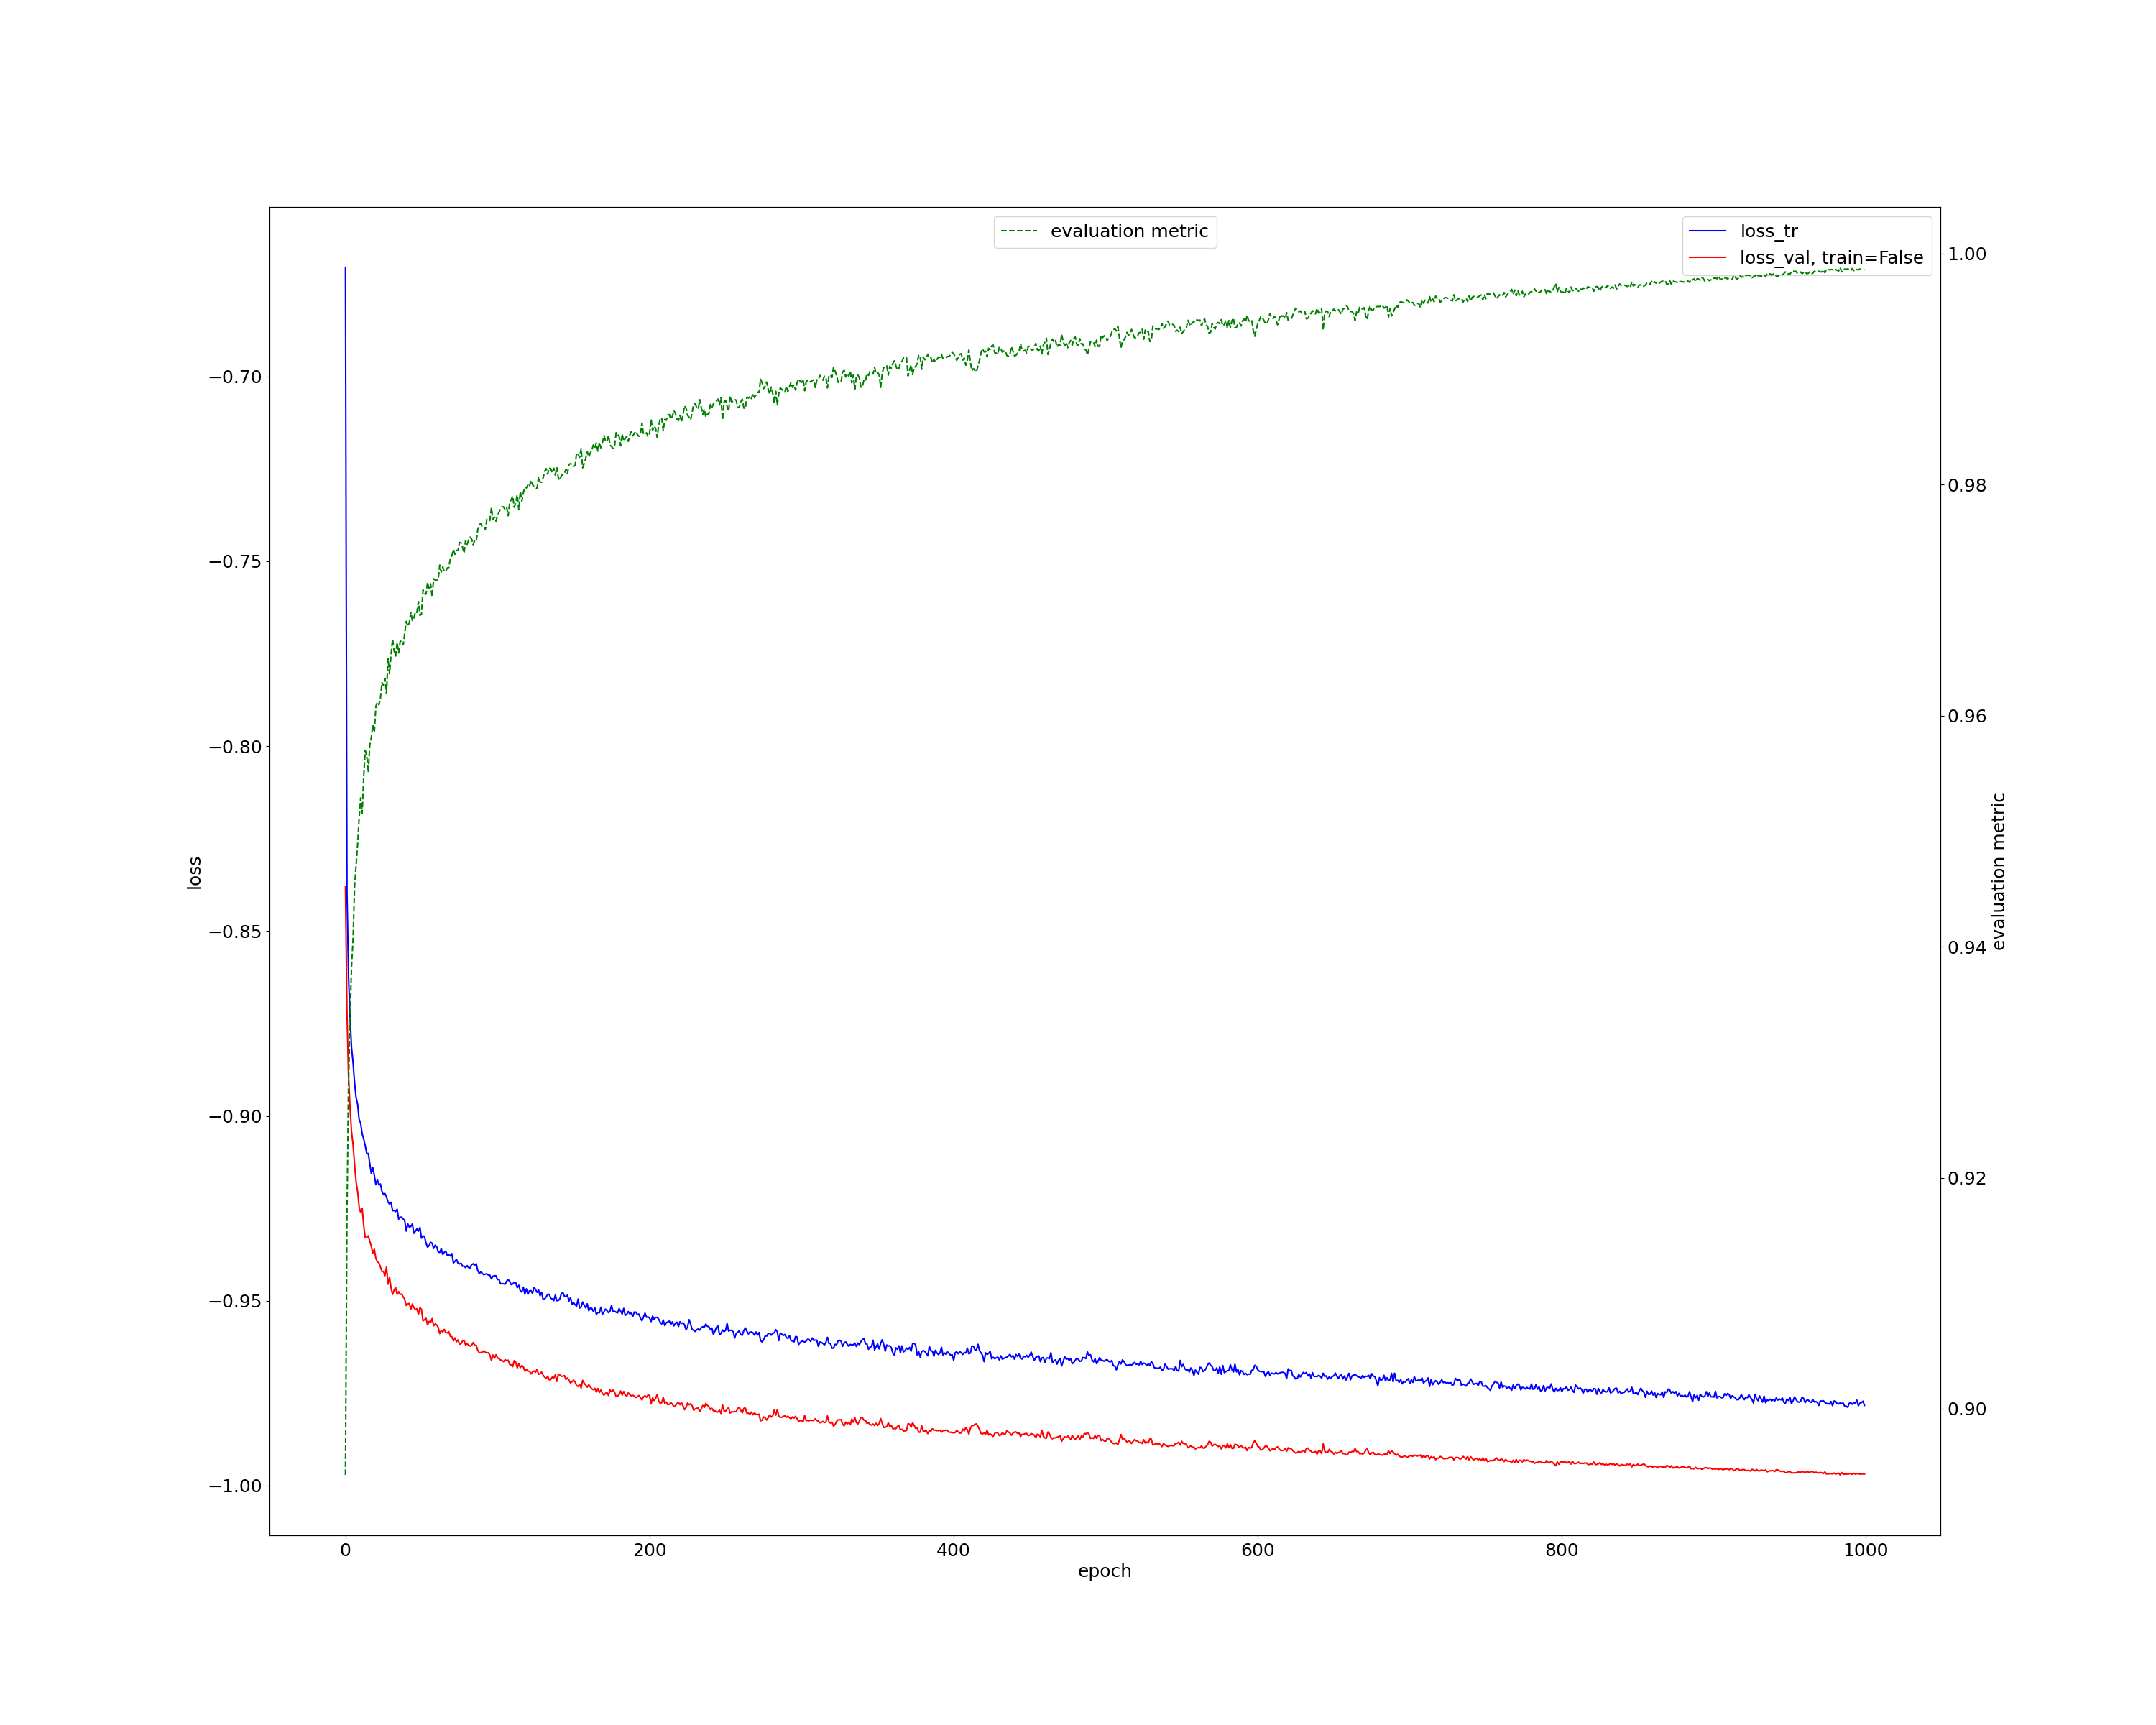
\includegraphics[width=\textwidth]{Pictures/nnUnet/Praxis/Task201-Larven-drittel-testsplit/progress_201-Larven-drittel-testsplit.png}
\caption{Verlauf des Dice-Koeffizienten beim Training über 1000 Epochen}
\label{pic:Prog_201}
\end{subfigure}
\end{minipage}%
\begin{minipage}{.4\textwidth}
\begin{subfigure}{\textwidth}
\includesvg[width=\textwidth]{Pictures/nnUnet/Praxis/Task201-Larven-drittel-testsplit/Scatterplot-Dice-201-Larven}
\caption{Scatterplot der Dice-Koeffizienten je Sample für Train- und Testsplit}
\label{pic:Dice_201}
\end{subfigure}
\end{minipage}

\caption{Dice-Koeffizienten zum Larvendatensatz mit einem Drittel als Testsplit}
\end{figure}

Bei der Visualisierung der Predictions fällt erneut auf, dass auf dem Trainsplit mit bloßem Auge keine Unterschiede zu Ground-Truth vorhanden sind (s. Abbildung \ref{pic:Vis-Train_201}), bei dem Testsplit kommt es jedoch bei den schlechtesten Beispielen zu Fehlern, die auch deutlich erkennbar sind. Es werden teilweise komplette Larven nicht oder nur teilweise erkannt und zudem wird auch besonders in den stark verschmutzen Bildern die Verschmutzung als Larve erkannt. Hierbei stellt sich die Frage, ob die Ground-Truth Segmentierung korrekt ist, da besonders die angeblichen Verschmutzungen, die das Modell als Larve erkannt hat, im Originalbild tatsächlich eher wie eine Larve aussehen als eine Verschmutzung. Intuitiv würde man die betroffenen Stellen im Originalbild vermutlich auch, wie das Modell, als Larve interpretieren. Die Larven die nicht erkannt wurden sind sehr schwach bis gar nicht mit dem Auge erkennbar bzw. ähneln stark einer Verschmutzung (s. Abbildung \ref{pic:Vis-Test_201}).

\begin{figure}[H]
\centering
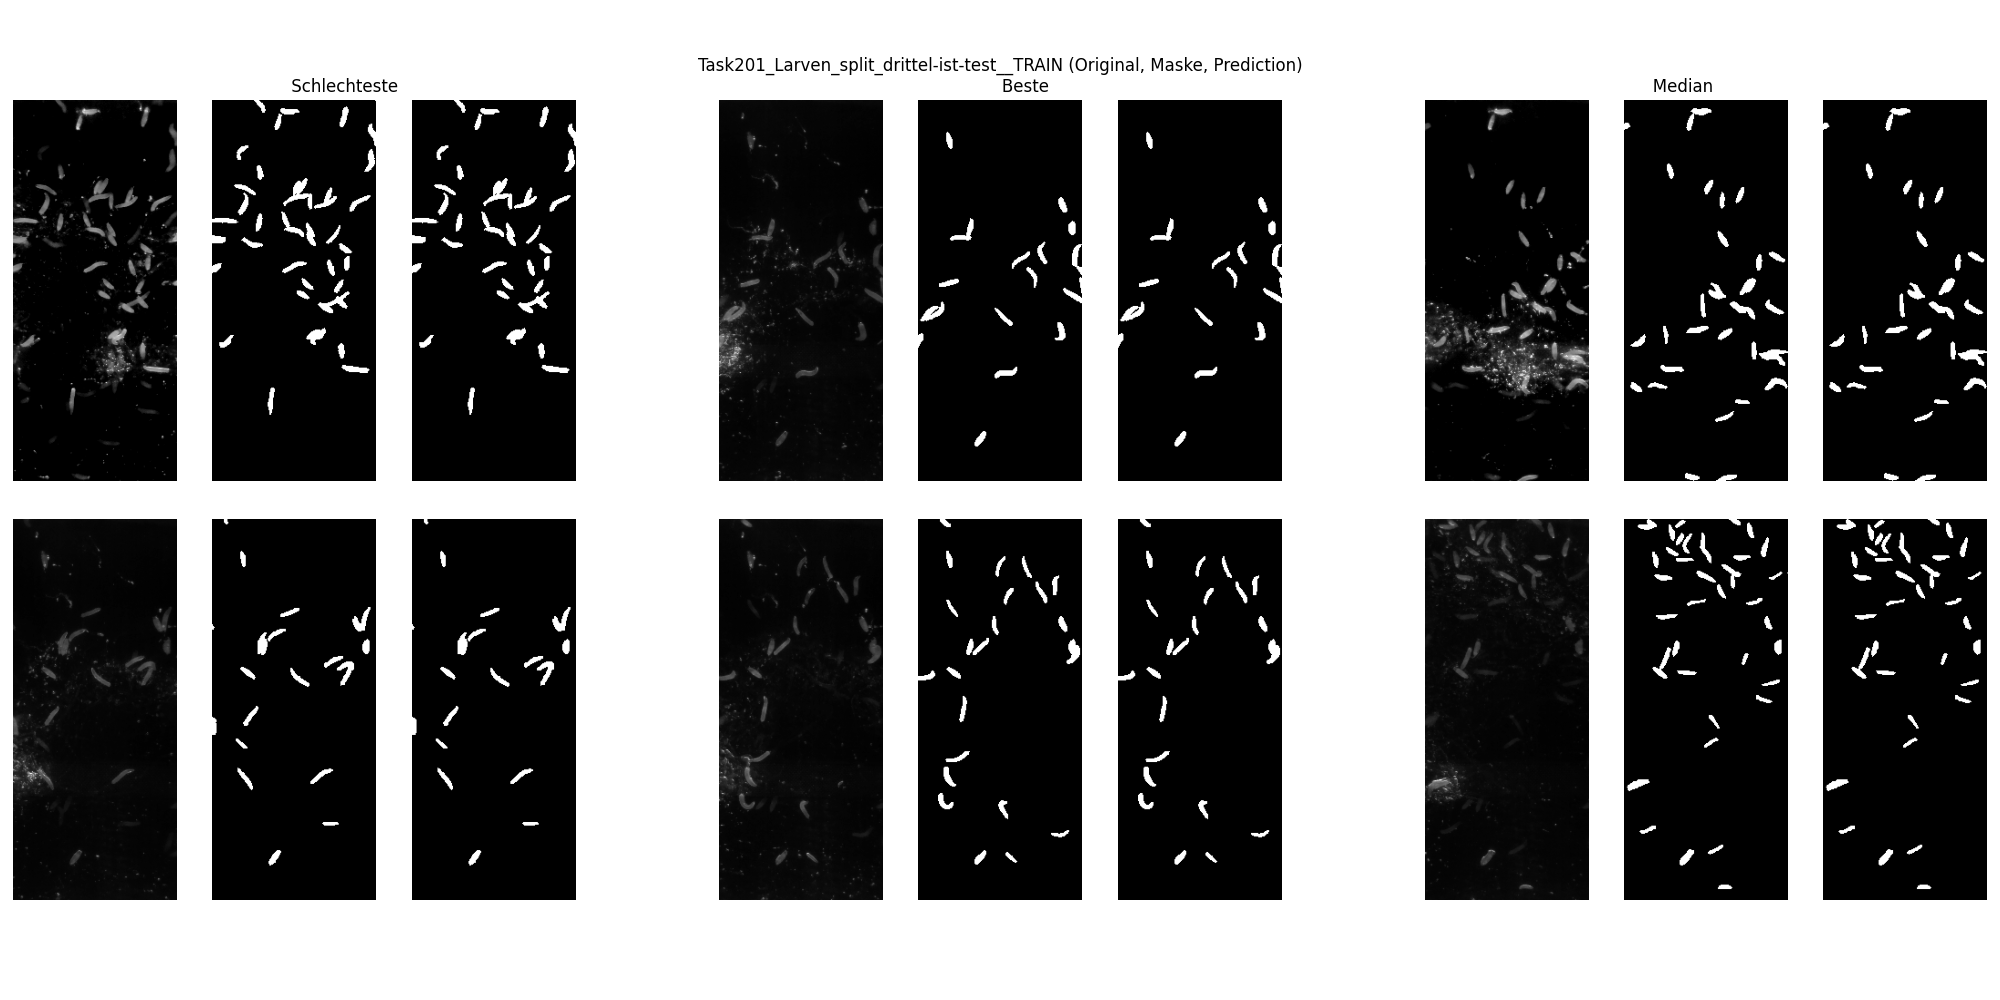
\includegraphics[height=0.35\textheight, width=\textwidth]{Pictures/nnUnet/Praxis/Task201-Larven-drittel-testsplit/Vis-Train.png}
\caption{Visualisierung des Trainsplits auf dem Larvendatensatz mit $\frac{1}{3}$ Testsplit (links: schlechteste Ergebnisse, mitte: beste Ergebnisse, rechts: Ergebnisse im Median; jeweils Original, Ground-Truth und Prediction)}
\label{pic:Vis-Train_201}
\end{figure}


\begin{figure}[H]
\centering
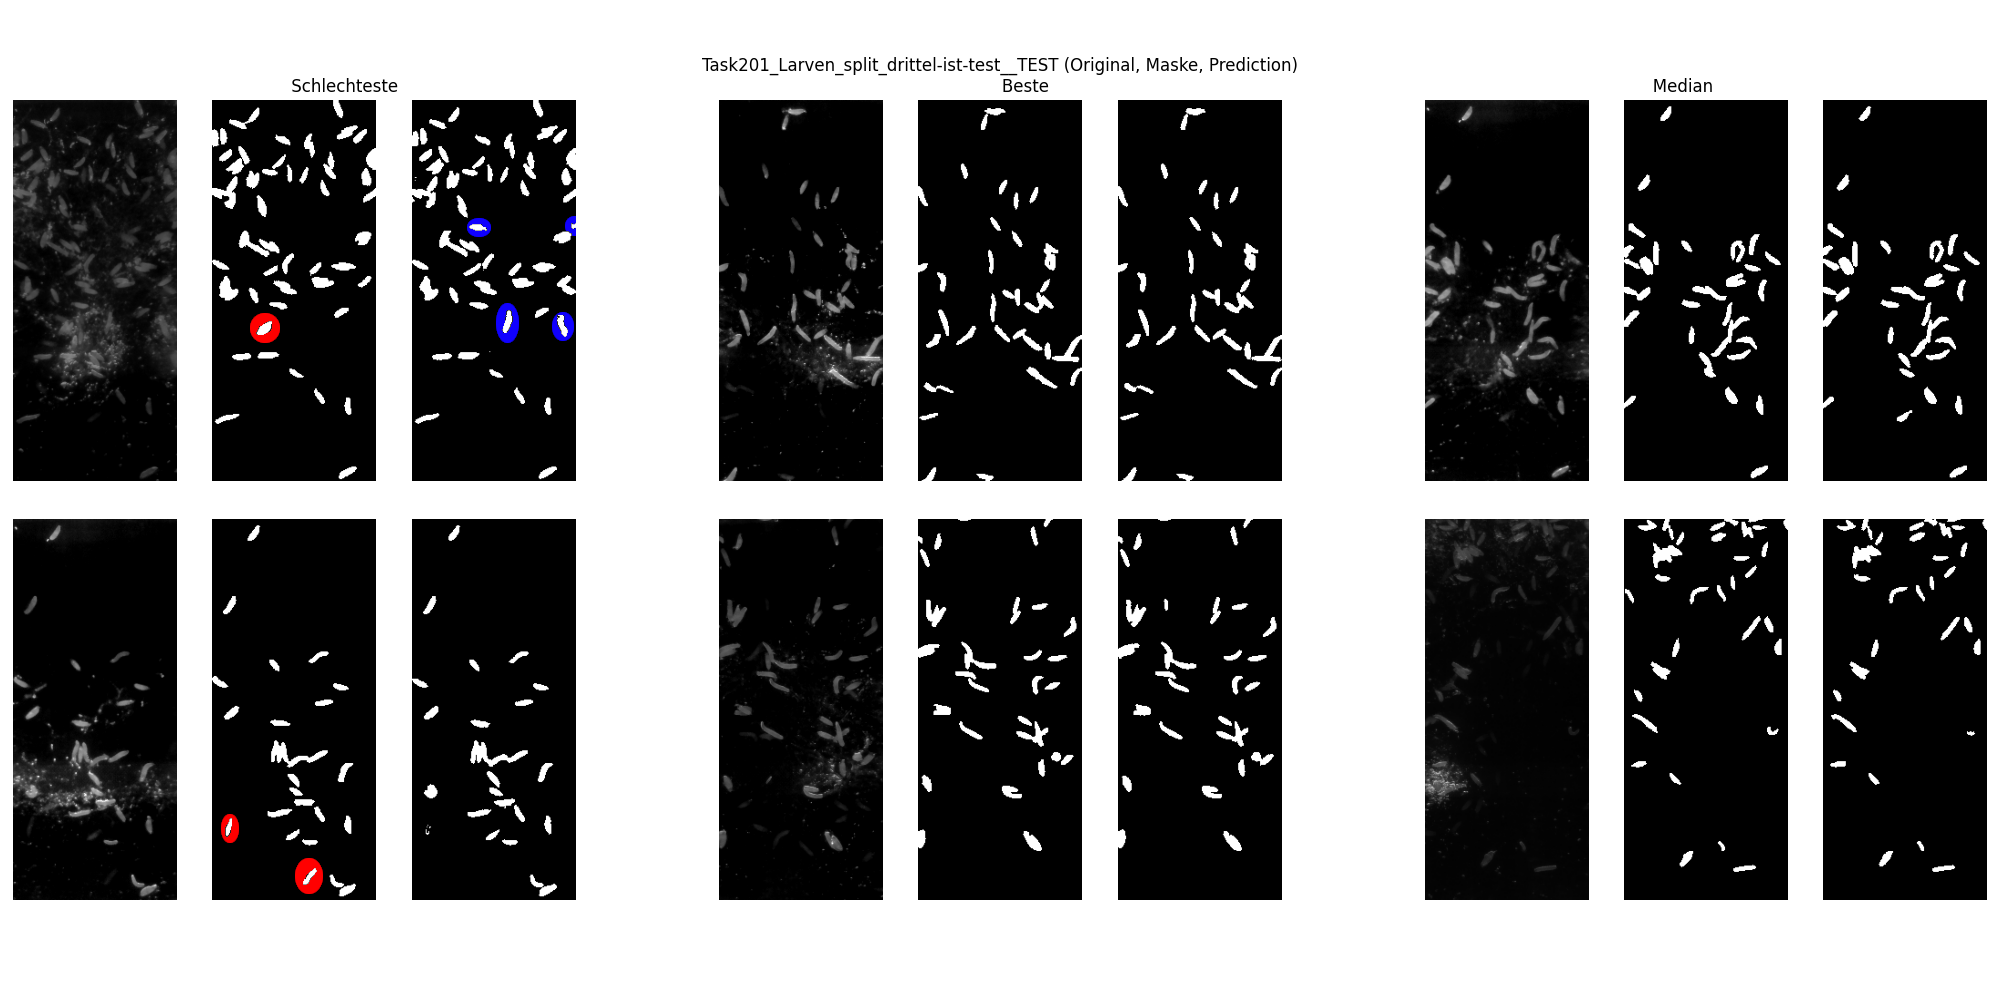
\includegraphics[height=0.35\textheight, width=\textwidth]{Pictures/nnUnet/Praxis/Task201-Larven-drittel-testsplit/Vis-Test-markiert.png}
\caption{Visualisierung des Testsplits auf dem Larvendatensatz mit $\frac{1}{3}$ Testsplit (links: schlechteste Ergebnisse, mitte: beste Ergebnisse, rechts: Ergebnisse im Median; jeweils Original, Ground-Truth und Prediction). Rot eingefärbt sind nicht erkannte Larven, blau als Larven erkannte Verschmutzungen}
\label{pic:Vis-Test_201}
\end{figure}


\subsection{Retina 2D-Datensatz}
\begin{figure}[H]
\begin{minipage}{.5\textwidth}
\begin{subfigure}{\textwidth}
\includesvg[width=\textwidth]{Pictures/nnUnet/Praxis/Task205-Augen-minimal-13-trainsamples/Haeufigkeitsverteilung-205-Retina2D-minimal-Train}
\caption{Trainsplit}
\label{pic:Haeuf-Train_205}
\end{subfigure}
\end{minipage}
\begin{minipage}{.5\textwidth}
\begin{subfigure}{\textwidth}
\includesvg[width=\textwidth]{Pictures/nnUnet/Praxis/Task205-Augen-minimal-13-trainsamples/Haeufigkeitsverteilung-205-Retina2D-minimal-Test}
\caption{Testsplit}
\label{pic:Haeuf-Test_205}
\end{subfigure}
\end{minipage}
\caption{Anteil von Objekt (Ader) je Sample mit Durchschnitt je Split $\approx$ 11-12\%}
\label{pic:Haeuf_205}
\end{figure}

Da wir auf dem Larven-Datensatz \cite{larven} (Graustufen mit einer einzigen Objekt-Klasse) so gute Ergebnisse erzielen konnten, obwohl das Framework für solche Aufgaben eigentlich nicht gemacht ist, wollten wir einen Schritt weiter gehen und statt graustufen Bildern farbige Bilder verwenden.\\
Dazu verwenden wir den Retina-2D Datensatz \cite{retina2d}. Dieser besteht aus jeweils 15 Aufnahmen von gesunden Retinae, Retinae von Augen mit Glaukom und diabetischer Retinopathie, also insgesamt 45 hochauflösenden RGB-Bildern. Unser Ziel der Segmentierung ist es, unabhängig von der Erkrankung, die Adern in der Retina zu markieren.\\
Diese Bilder konnten auch wie bei den Larven mit dem zur Verfügung gestellten Python-Script \cite{nnunetGithub2D-Pythonscript} in Nifti-Dateien konvertiert werden. Jedoch ergab sich beim Ausführen des Trainings das Problem, dass die automatisch ermittelte Batch-Size des Frameworks angeblich zu niedrig ist. Nach etwas Ausprobieren und Nachschauen im Code sind wir auf eine \enquote{estimated GPU-RAM consumption} \cite{nnunetGithub} gestoßen, die die Batch-Size vorgibt. Durch die hohe Auflösung der Bilder ($\approx$ 3500x2300) und den 3 Farbkanälen wird dieser geschätzte GPU-Ram Verbrauch zu groß und als Folge dessen die Batch-Size mit 1 zu klein, da in einem Batch per Definition des Frameworks immer mindestens 2 Samples enthalten sein müssen.\\
Durch Ausgeben des geschätzten GPU-Ram Verbrauchs haben wir herausgefunden, dass dieser ungefähr linear mit der Anzahl an Pixeln wächst und konnten so ausrechnen, dass eine Verkleinerung der Bilder auf mindestens 42\% ausreicht, damit 2 Samples in ein Batch gelangen können.
Diese Verkleinerung der Auflösung muss nur für die Trainingsdaten vorgenommen werden. Auf den Testdaten, von denen lediglich eine Prediction erstellt werden muss, kann die Auflösung höher sein.\\
Außerdem haben wir, bevor wir mit dem geschätzten GPU-Ram Verbrauch gespielt haben, manuelle Data-Augmentation betrieben indem wir die Bilder rotiert und gespiegelt haben, in der Hoffnung dadurch mehr Samples in einem Batch zu erhalten. Dies hat sich im Nachhinein jedoch als nicht nötig herausgestellt und hat dem Framework das Training im 1. Durchlauf eventuell unnötig erschwert. Später im 2. Durchlauf mit minimaler Trainingssample-Anzahl haben wir diesen Fehler nicht gemacht.


\begin{figure}[H]
\centering
\begin{minipage}{.6\textwidth}
\begin{subfigure}{\textwidth}
\centering
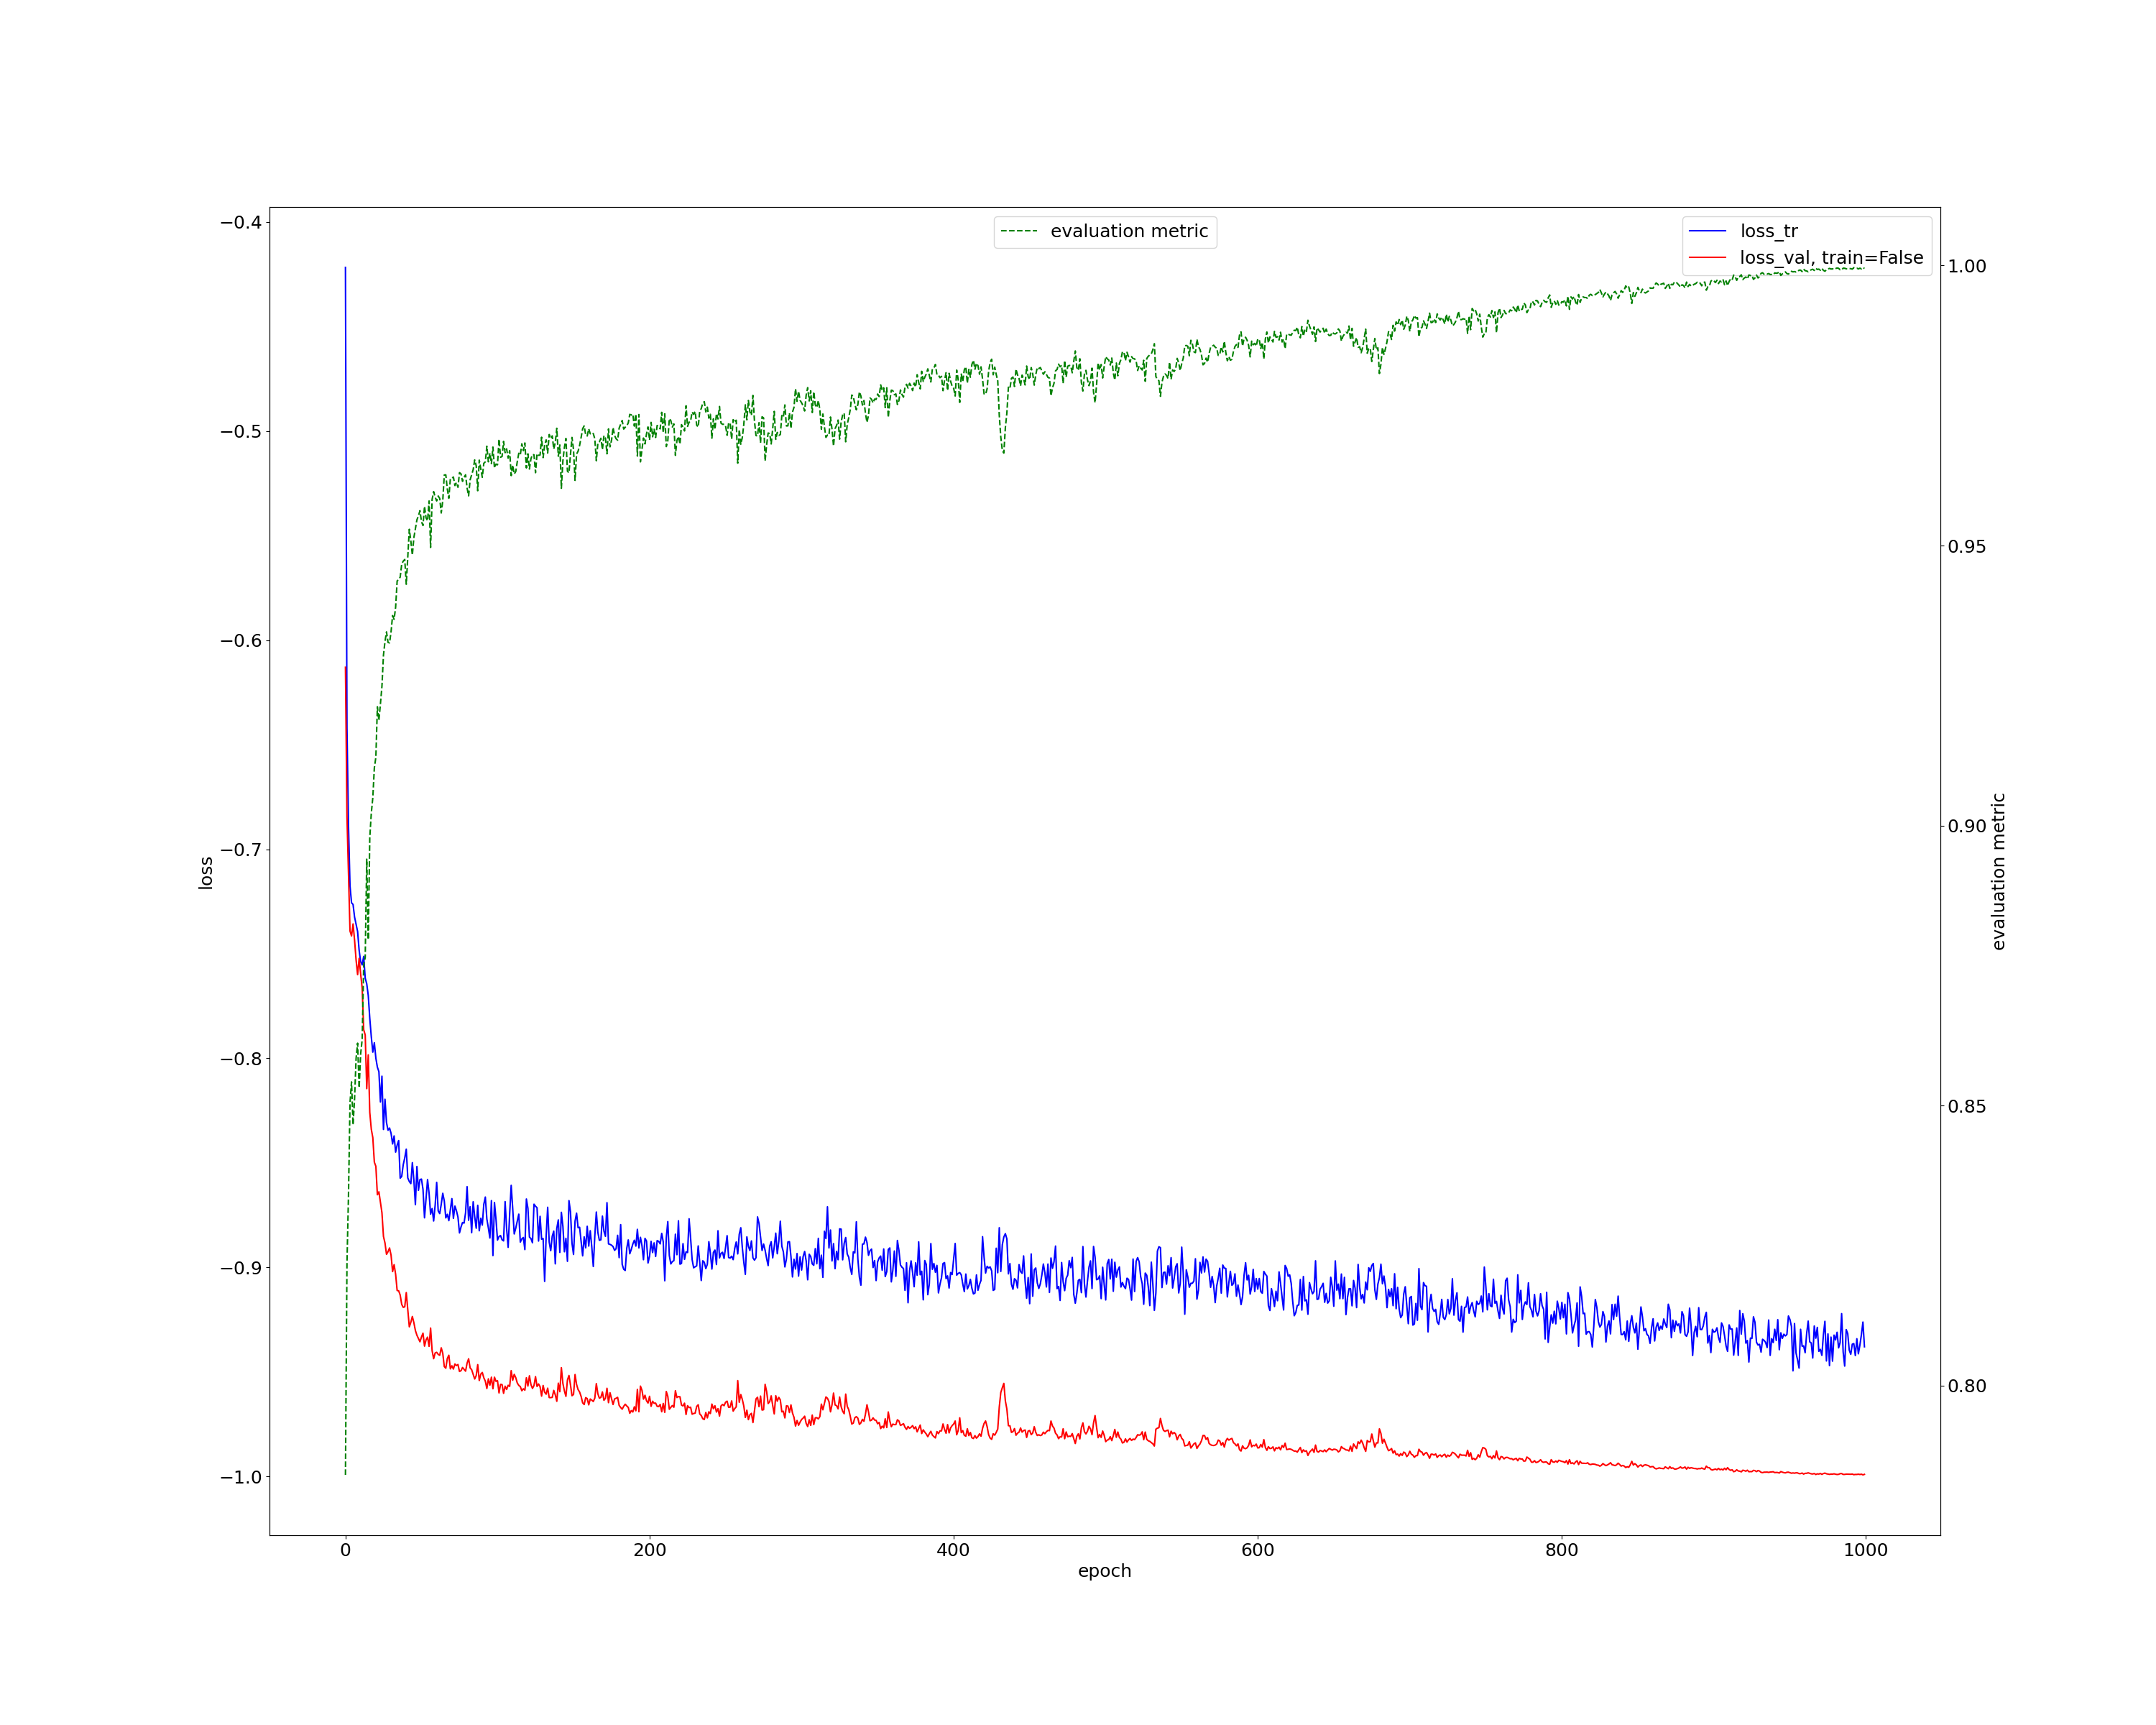
\includegraphics[width=\textwidth]{Pictures/nnUnet/Praxis/Task203-Augen-drittel-testsplit/progress_203-Augen-drittel-split.png}
\caption{Verlauf des Dice-Koeffizienten beim Training über 1000 Epochen}
\label{pic:Prog_203}
\end{subfigure}
\end{minipage}%
\begin{minipage}{.4\textwidth}
\begin{subfigure}{\textwidth}
\includesvg[width=\textwidth]{Pictures/nnUnet/Praxis/Task203-Augen-drittel-testsplit/Scatterplot-Dice-203}
\caption{Scatterplot der Dice-Koeffizienten je Sample für Train- und Testsplit}
\label{pic:Dice_203}
\end{subfigure}
\end{minipage}

\caption{Dice-Koeffizienten zum Retina-2D Datensatz \cite{retina2d} mit einem Drittel als Testsplit}
\end{figure}

Da wir auch hier relativ gute Ergebnisse erzielen konnten, wollten wir das Framework an seine Grenzen bringen und so wenig Trainingsamples wie möglich zur Verfügung stellen. Durch Ausprobieren und schrittweises Annähern haben wir herausgefunden, dass nnUNet, jedenfalls bei diesem Datensatz, mindestens 13 Trainingsbeispiele benötigt, da bei weniger Trainingsbeispielen später beim Training ein \textit{IndexOutOfBounds} Fehler auftritt. Leider ist beim Aufteilen in Train- und Testsplit der Objektanteil in den Samples nicht ganz ausbalanciert, da im Trainsplit nur 11\% der Pixel Adern sind und im Testsplit knapp 12\% (s. Abbildung \ref{pic:Haeuf_205}).


\begin{figure}[H]
\centering
\begin{minipage}{.6\textwidth}
\begin{subfigure}{\textwidth}
\centering
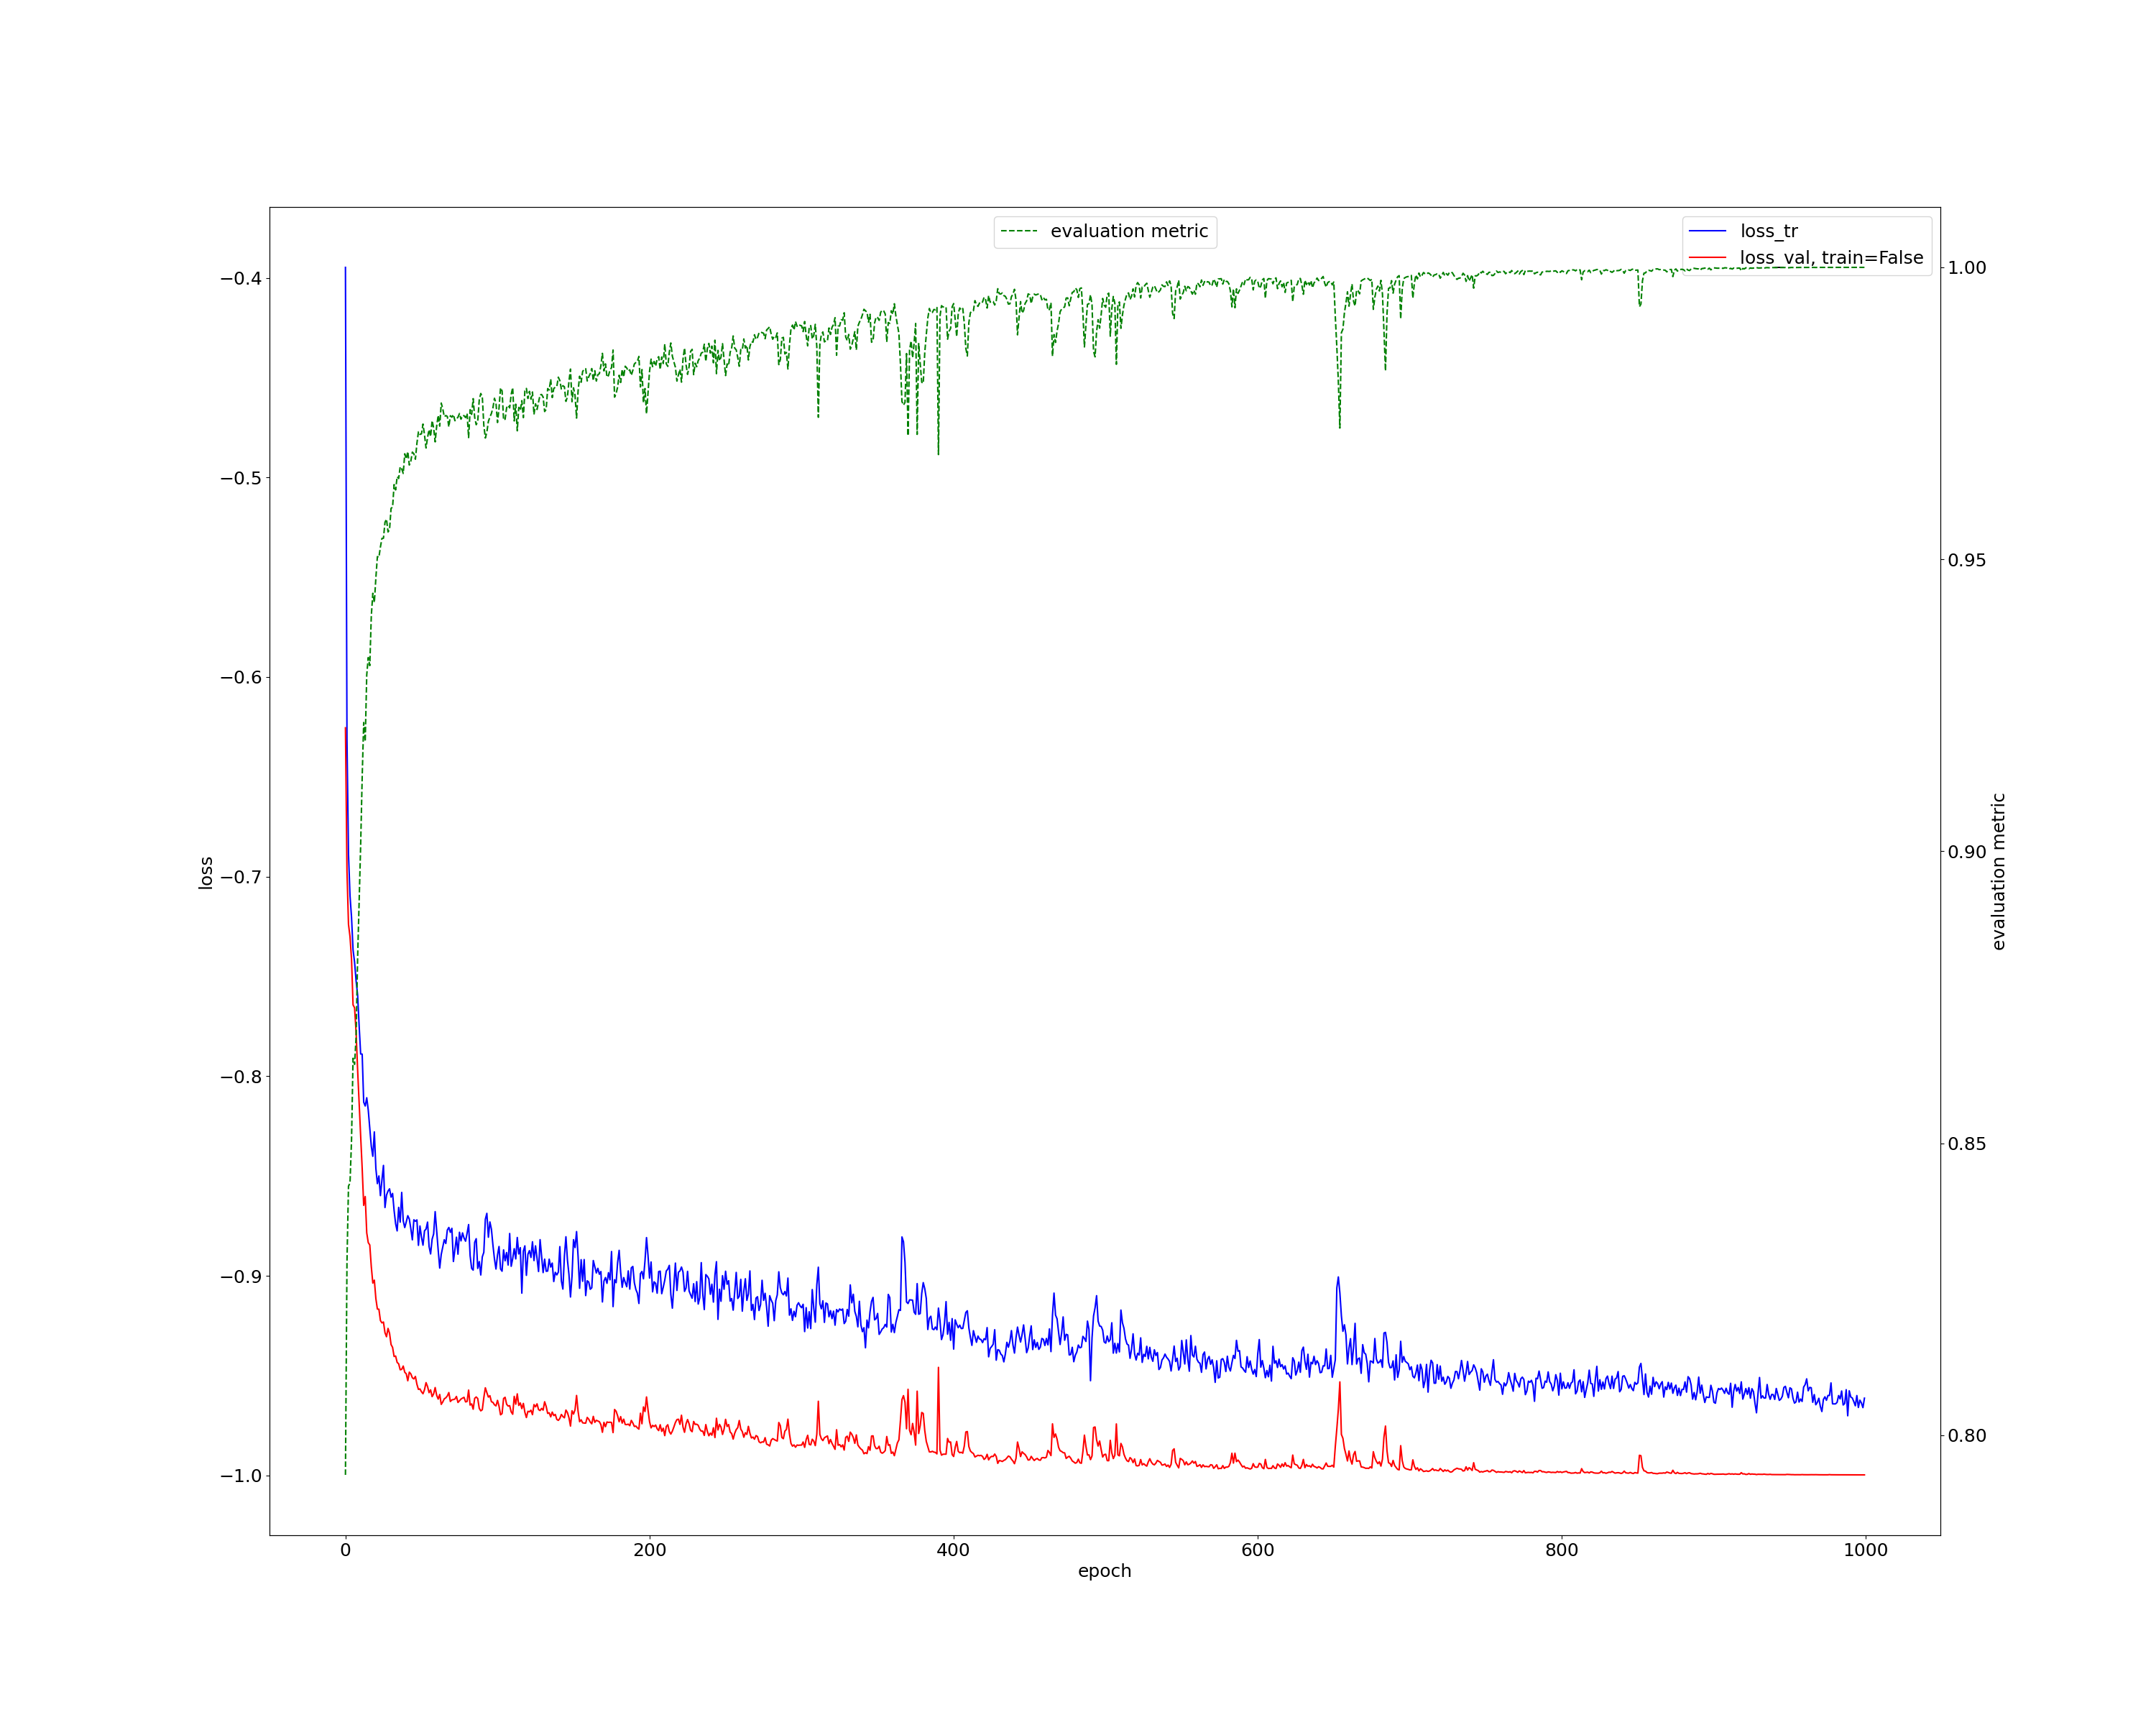
\includegraphics[width=\textwidth]{Pictures/nnUnet/Praxis/Task205-Augen-minimal-13-trainsamples/progress_205-Augen-minimal-13-trainsamples.png}
\caption{Verlauf des Dice-Koeffizienten beim Training über 1000 Epochen}
\label{pic:Prog_205}
\end{subfigure}
\end{minipage}%
\begin{minipage}{.4\textwidth}
\begin{subfigure}{\textwidth}
\includesvg[width=\textwidth]{Pictures/nnUnet/Praxis/Task205-Augen-minimal-13-trainsamples/Scatterplot-Dice-205}
\caption{Scatterplot der Dice-Koeffizienten je Sample für Train- und Testsplit}
\label{pic:Dice_205}
\end{subfigure}
\end{minipage}

\caption{Dice-Koeffizienten zum Retina-2D Datensatz mit einem minimalen Trainsplit von 13 Samples}
\end{figure}


Es fällt auf, dass bei dem minimalen Trainingssplit Overfitting stattfindet, da alle Samples bis auf ein einziges einen Dice-Koeffizienten von genau 1 besitzen (s. Abbildung \ref{pic:Dice_205}). Auch der Progress-Graph (Abbildung \ref{pic:Prog_205}) steigt am Anfang schneller als bei $\frac{2}{3}$ Trainingssplit.\\
Auf dem Testsplit fällt auf, dass bei Durchlauf 1 (Abbildung \ref{pic:Dice_203}) eine Gruppierung stattfindet. Viele Samples liegen sehr nah bei 1 und eine zweite, etwa gleich große Gruppe liegt um $0,85$ herum. Dies kommt sehr wahrscheinlich von unserer, fälschlicherweise durchgeführten, manuellen Data-Augmentation, bei der wir das gleiche Bild mehrmals in rotierter und gespiegelter Form in das Framework gegeben haben. Beim 2. Durchlauf mit minimalem Trainsplit sind die Samples im Testsplit relativ gleichmäßig um den Durchschnitt von $0,83$ verteilt (s. Abbildung \ref{pic:Dice_205}).\\\\
Beim Betrachten der Visualisierung der besten, schlechtesten und mittleren Predictions je Split (Abbildungen \ref{pic:Vis-Train_205}, \ref{pic:Vis-Test_205}) fällt auf, dass die Adern in der Predictions generell breiter sind als in Ground-Truth. Das kommt von der leider notwendigen Verkleinerung der Auflösung der Bilder, da dann bei feinen Adern anstatt nur schwarzer oder weißer Pixel in der Ground-Truth Segmentierung auch graue Pixel entstehen, da z.B. Adern mit einer Breite von einem Pixel nicht weiter in der Auflösung reduziert werden können. Wir haben uns dafür entschieden, die dann grauen Pixel auch als weiße Pixel, also als Ader-Segmentierung, zu zählen, da ansonsten feine Adern Lücken bekommen und die Segmentierung insgesamt schlechter ausfällt. Wenn das Framework wie geplant zu einem späteren Zeitpunkt Patches in der 2D-Variante erlaubt, wäre eine Verkleinerung der Auflösung nicht mehr nötig und das Problem der zu breiten Adern nicht mehr vorhanden \cite{nnunetGithub-2dpatches}.
Ansonsten findet man keine groben Fehler, die meisten Adern werden sehr genau erkannt. 



\begin{figure}[H]
\centering
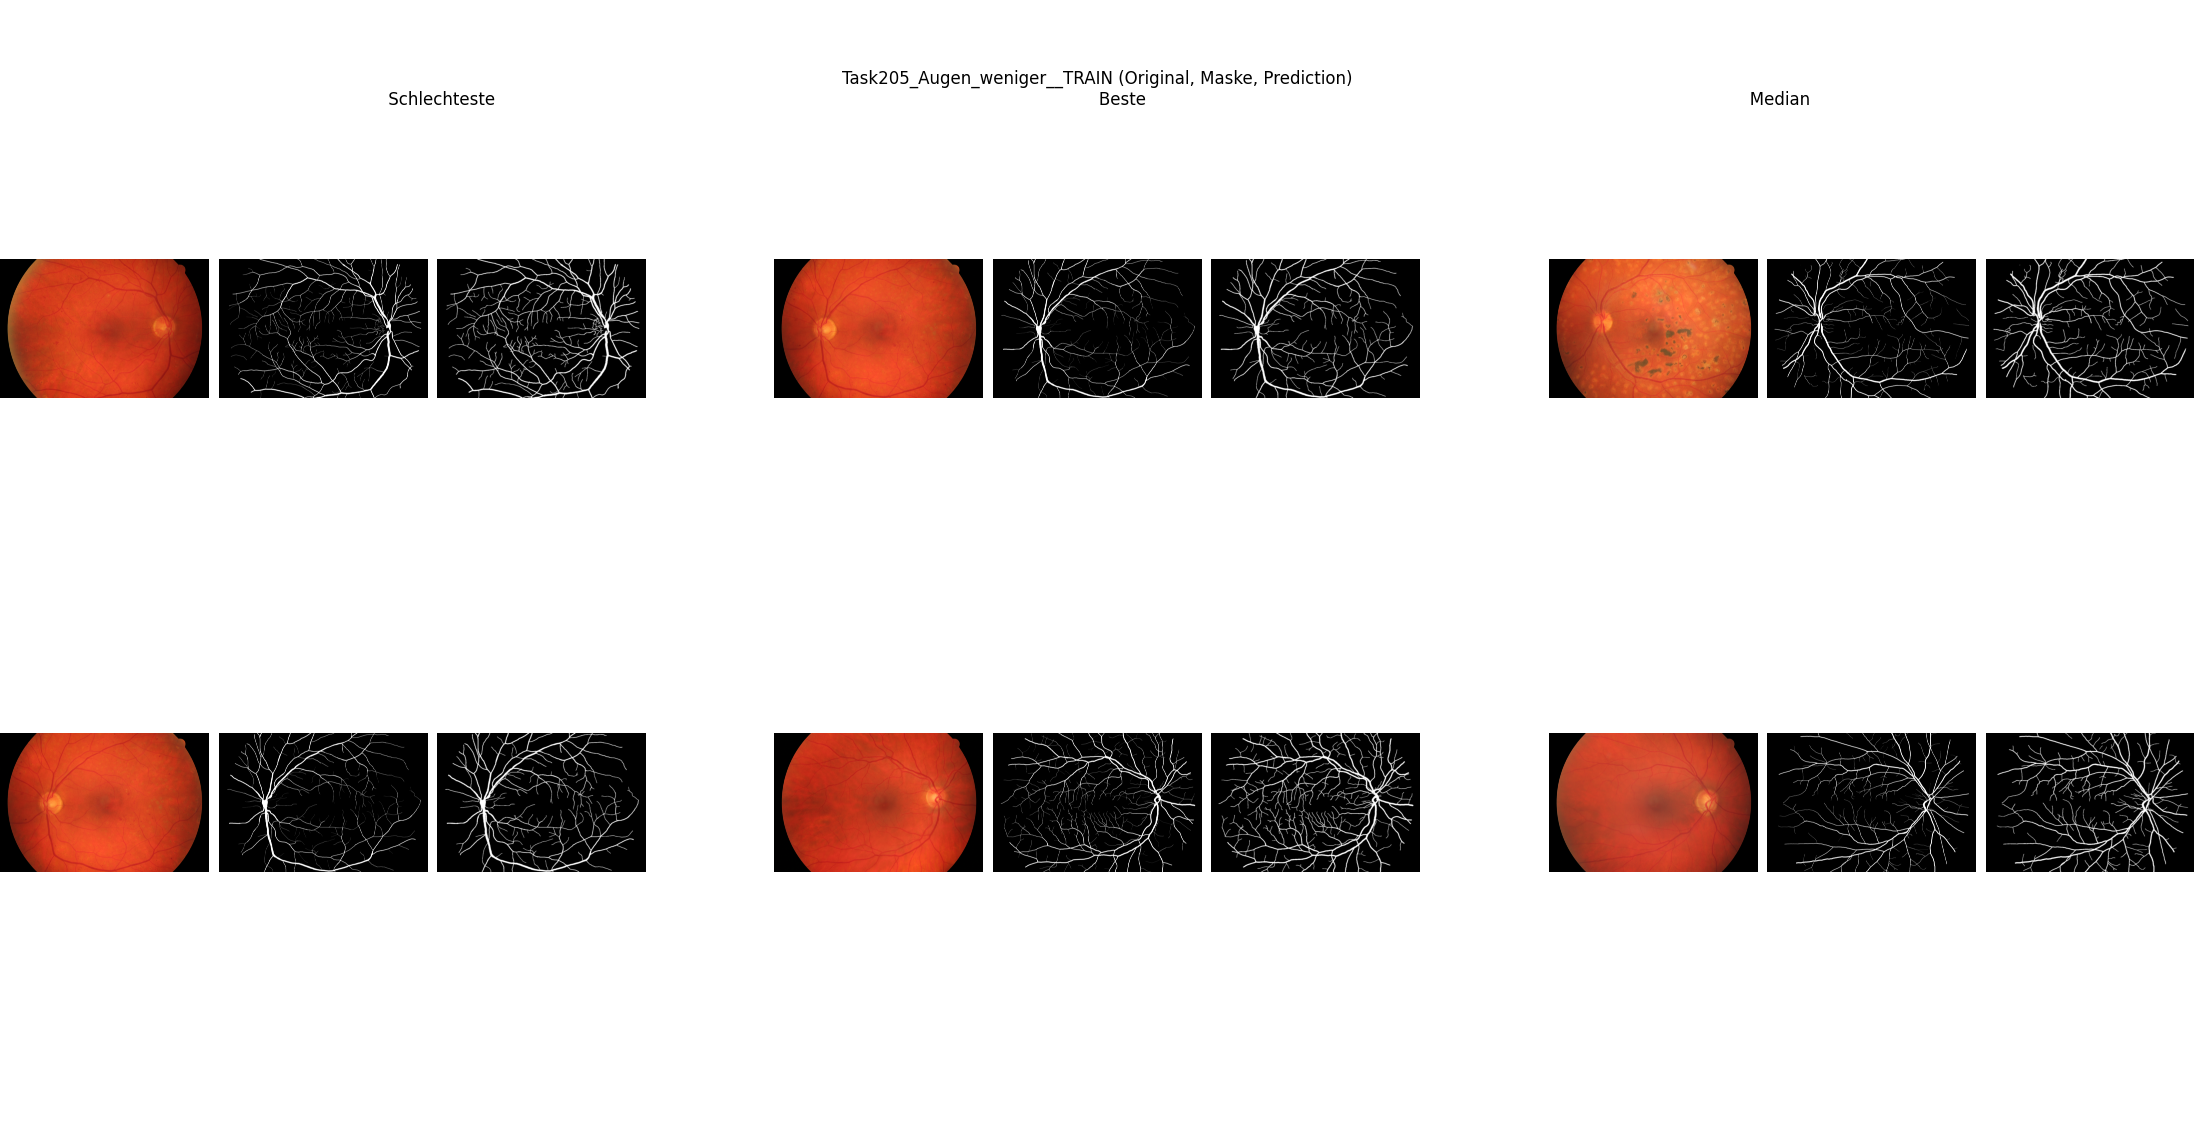
\includegraphics[height=0.35\textheight, width=\textwidth]{Pictures/nnUnet/Praxis/Task205-Augen-minimal-13-trainsamples/Vis-Train.png}
\caption{Visualisierung des Trainsplits auf dem Retina-Datensatz mit minimalem Trainsplit (links: schlechteste Ergebnisse, mitte: beste Ergebnisse, rechts: Ergebnisse im Median; jeweils Original, Ground-Truth und Prediction)}
\label{pic:Vis-Train_205}
\end{figure}


\begin{figure}[H]
\centering
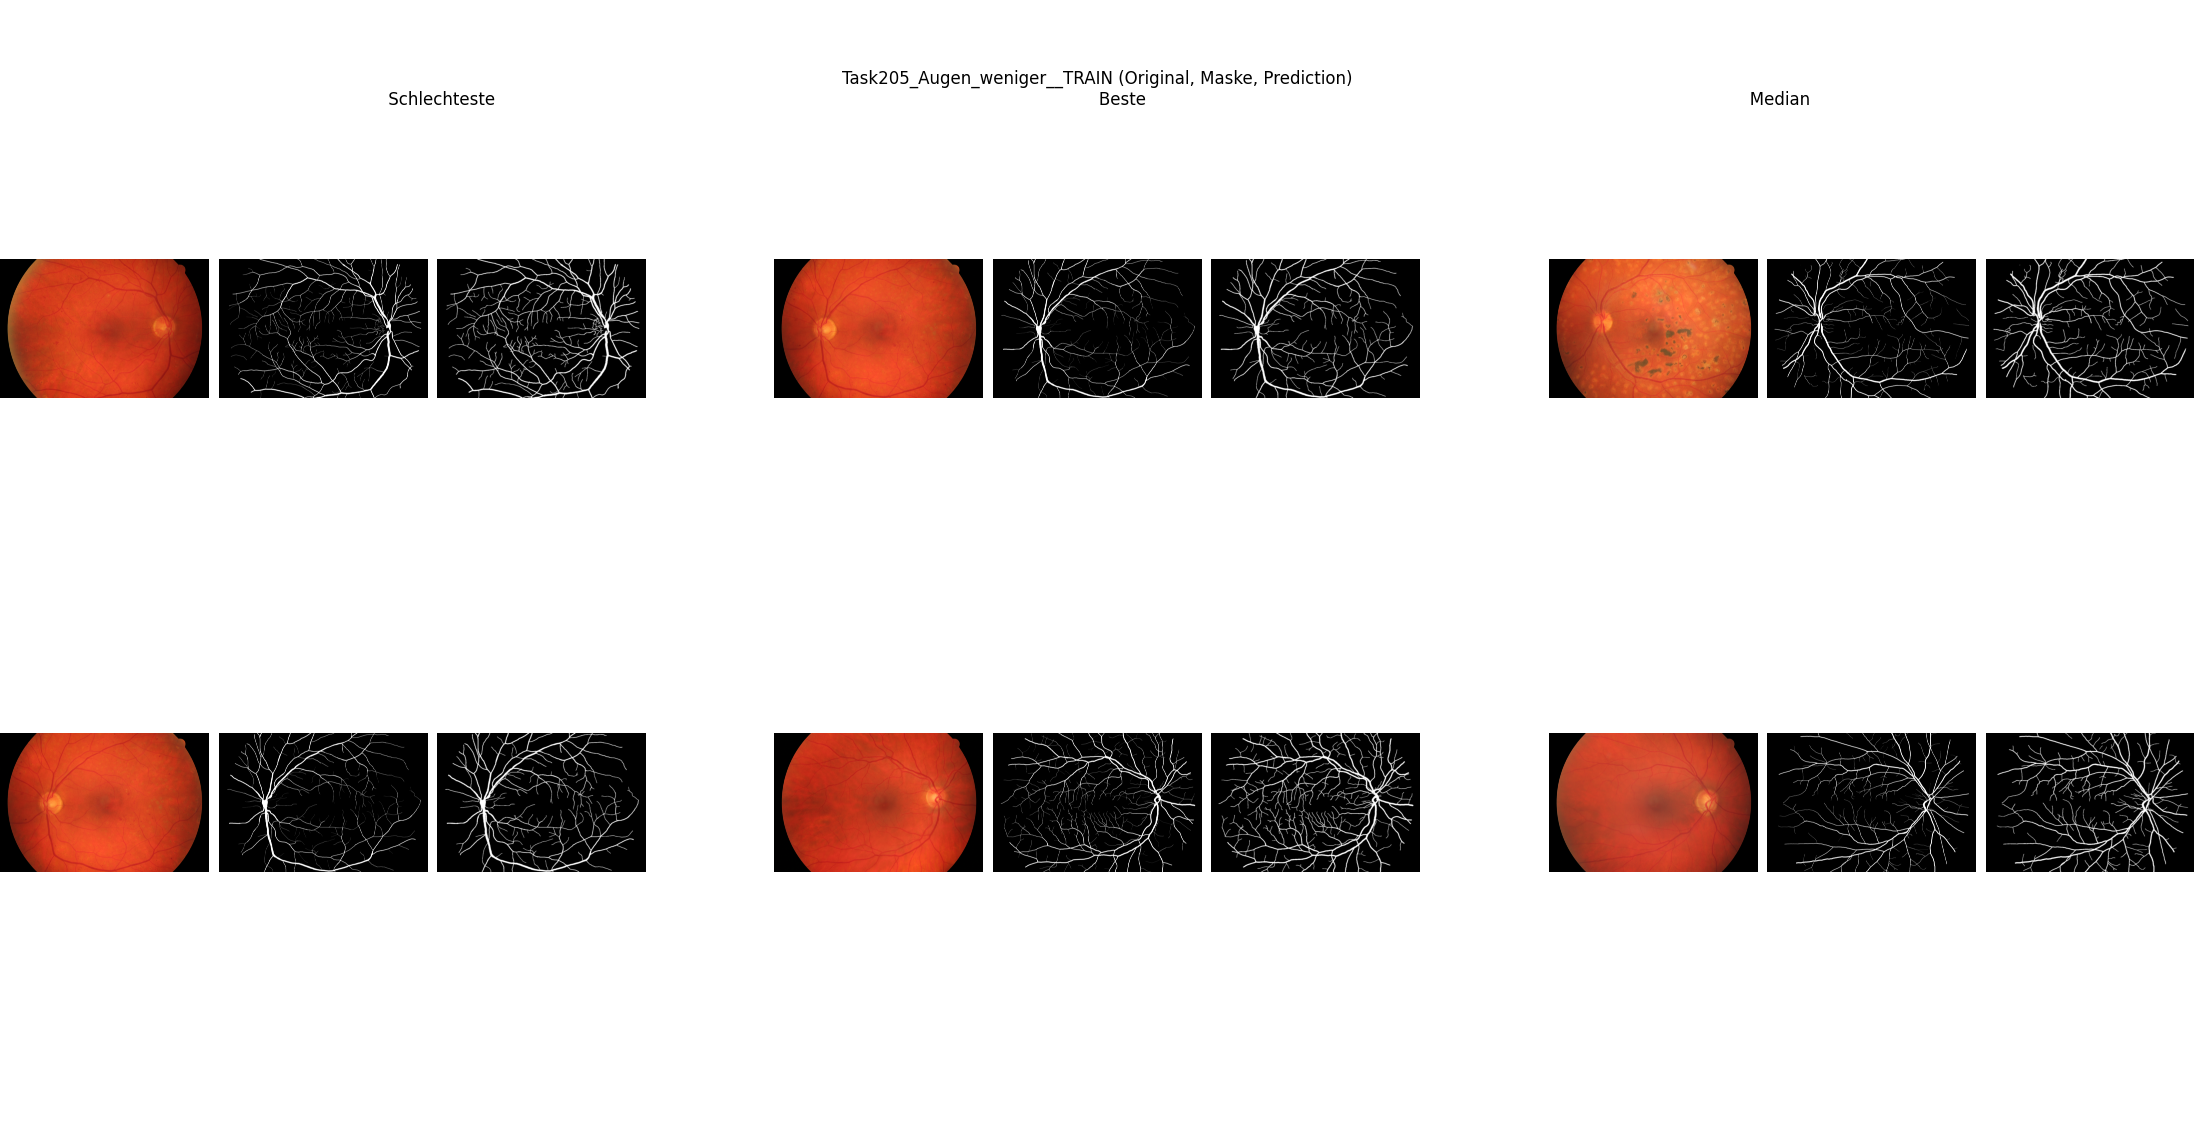
\includegraphics[height=0.35\textheight, width=\textwidth]{Pictures/nnUnet/Praxis/Task205-Augen-minimal-13-trainsamples/Vis-Train.png}
\caption{Visualisierung des Testsplits auf dem Retina-Datensatz mit minimalem Trainsplit (links: schlechteste Ergebnisse, mitte: beste Ergebnisse, rechts: Ergebnisse im Median; jeweils Original, Ground-Truth und Prediction)}
\label{pic:Vis-Test_205}
\end{figure}





Da wir bei diesem Datensatz relativ gute Ergebnisse produzieren konnten, haben wir dem Framework komplett fremde Bilder \cite{retina2dExtra} in verschiedenen Auflösungen und Zoom-Stufen zum Segmentieren gegeben. Zu diesen Bildern gab es leider keine Ground-Truth Segmentierung, jedoch kann man auch so grob abschätzen wie robust das Modell ist, und dass es tatsächlich die Merkmale einer Ader in der Retina erlernt hat und sogar mit verschiedenen Auflösungen, Ausschnitten und \textit{Färbungen} der Retina umgehen kann (s. Abbildung \ref{pic:retinaExtraA} und \ref{pic:retinaExtraB}).
\begin{figure}[H]

\begin{minipage}{.5\textwidth}
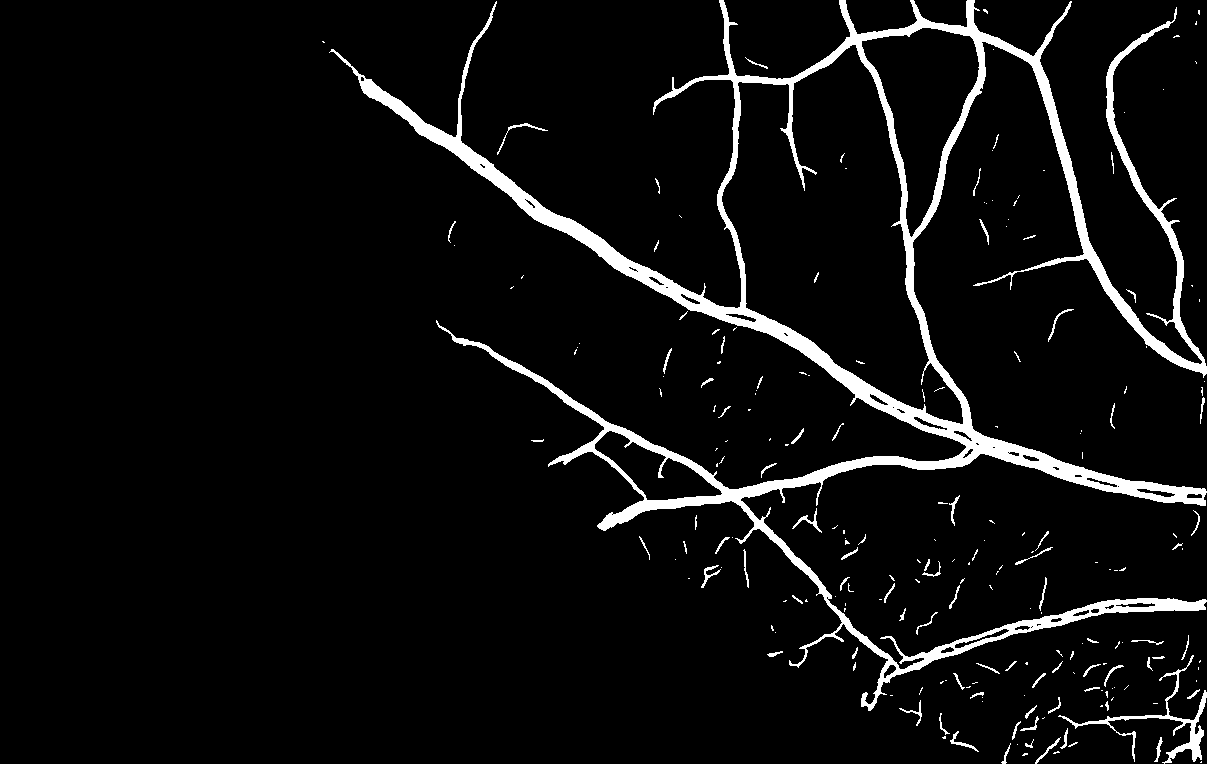
\includegraphics[width=\textwidth]{Pictures/nnUnet/Praxis/Task205-Augen-minimal-13-trainsamples/extra_Bilder/13a_right_cut.png}
\end{minipage}
\begin{minipage}{.5\textwidth}
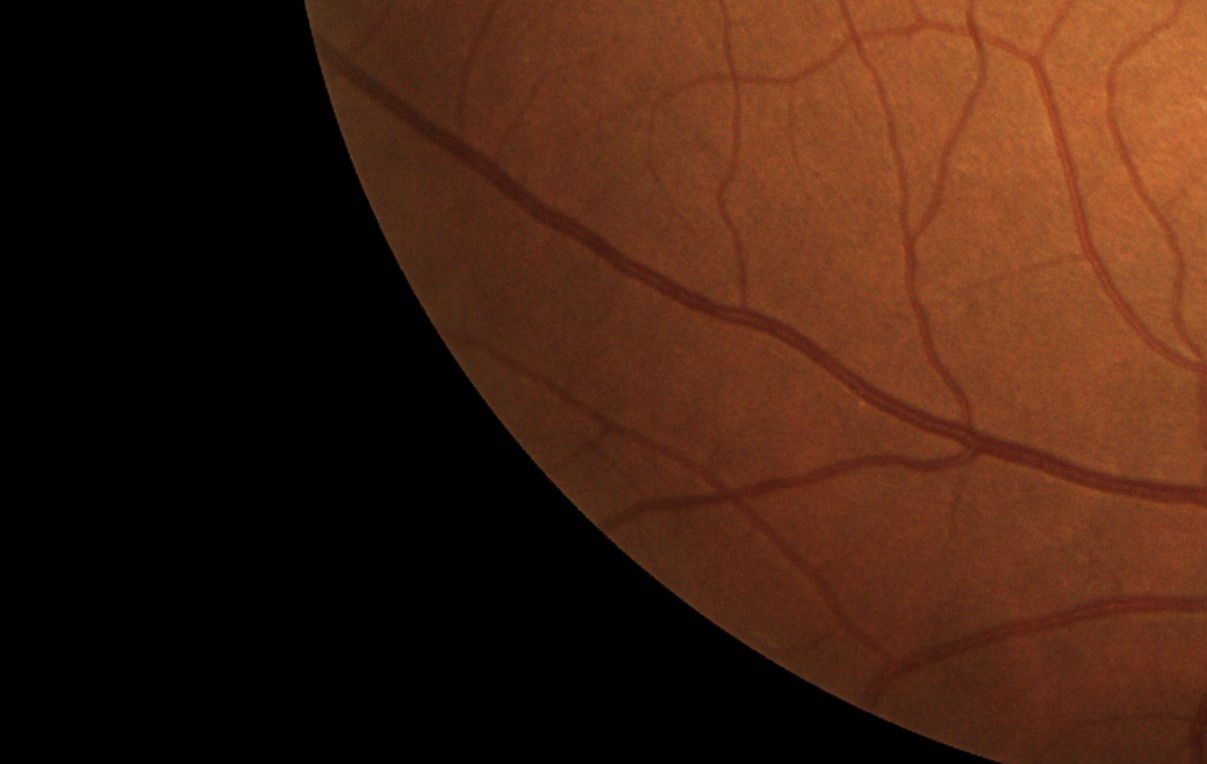
\includegraphics[width=\textwidth]{Pictures/nnUnet/Praxis/Task205-Augen-minimal-13-trainsamples/extra_Bilder/13a_right_cut-original.jpeg}
\end{minipage}
\caption{Bild 13a\_right aus \cite{retina2dExtra} in starkem Zoom - Prediction und Original}
\label{pic:retinaExtraA}
\end{figure}

\begin{figure}[H]
\begin{minipage}{.5\textwidth}
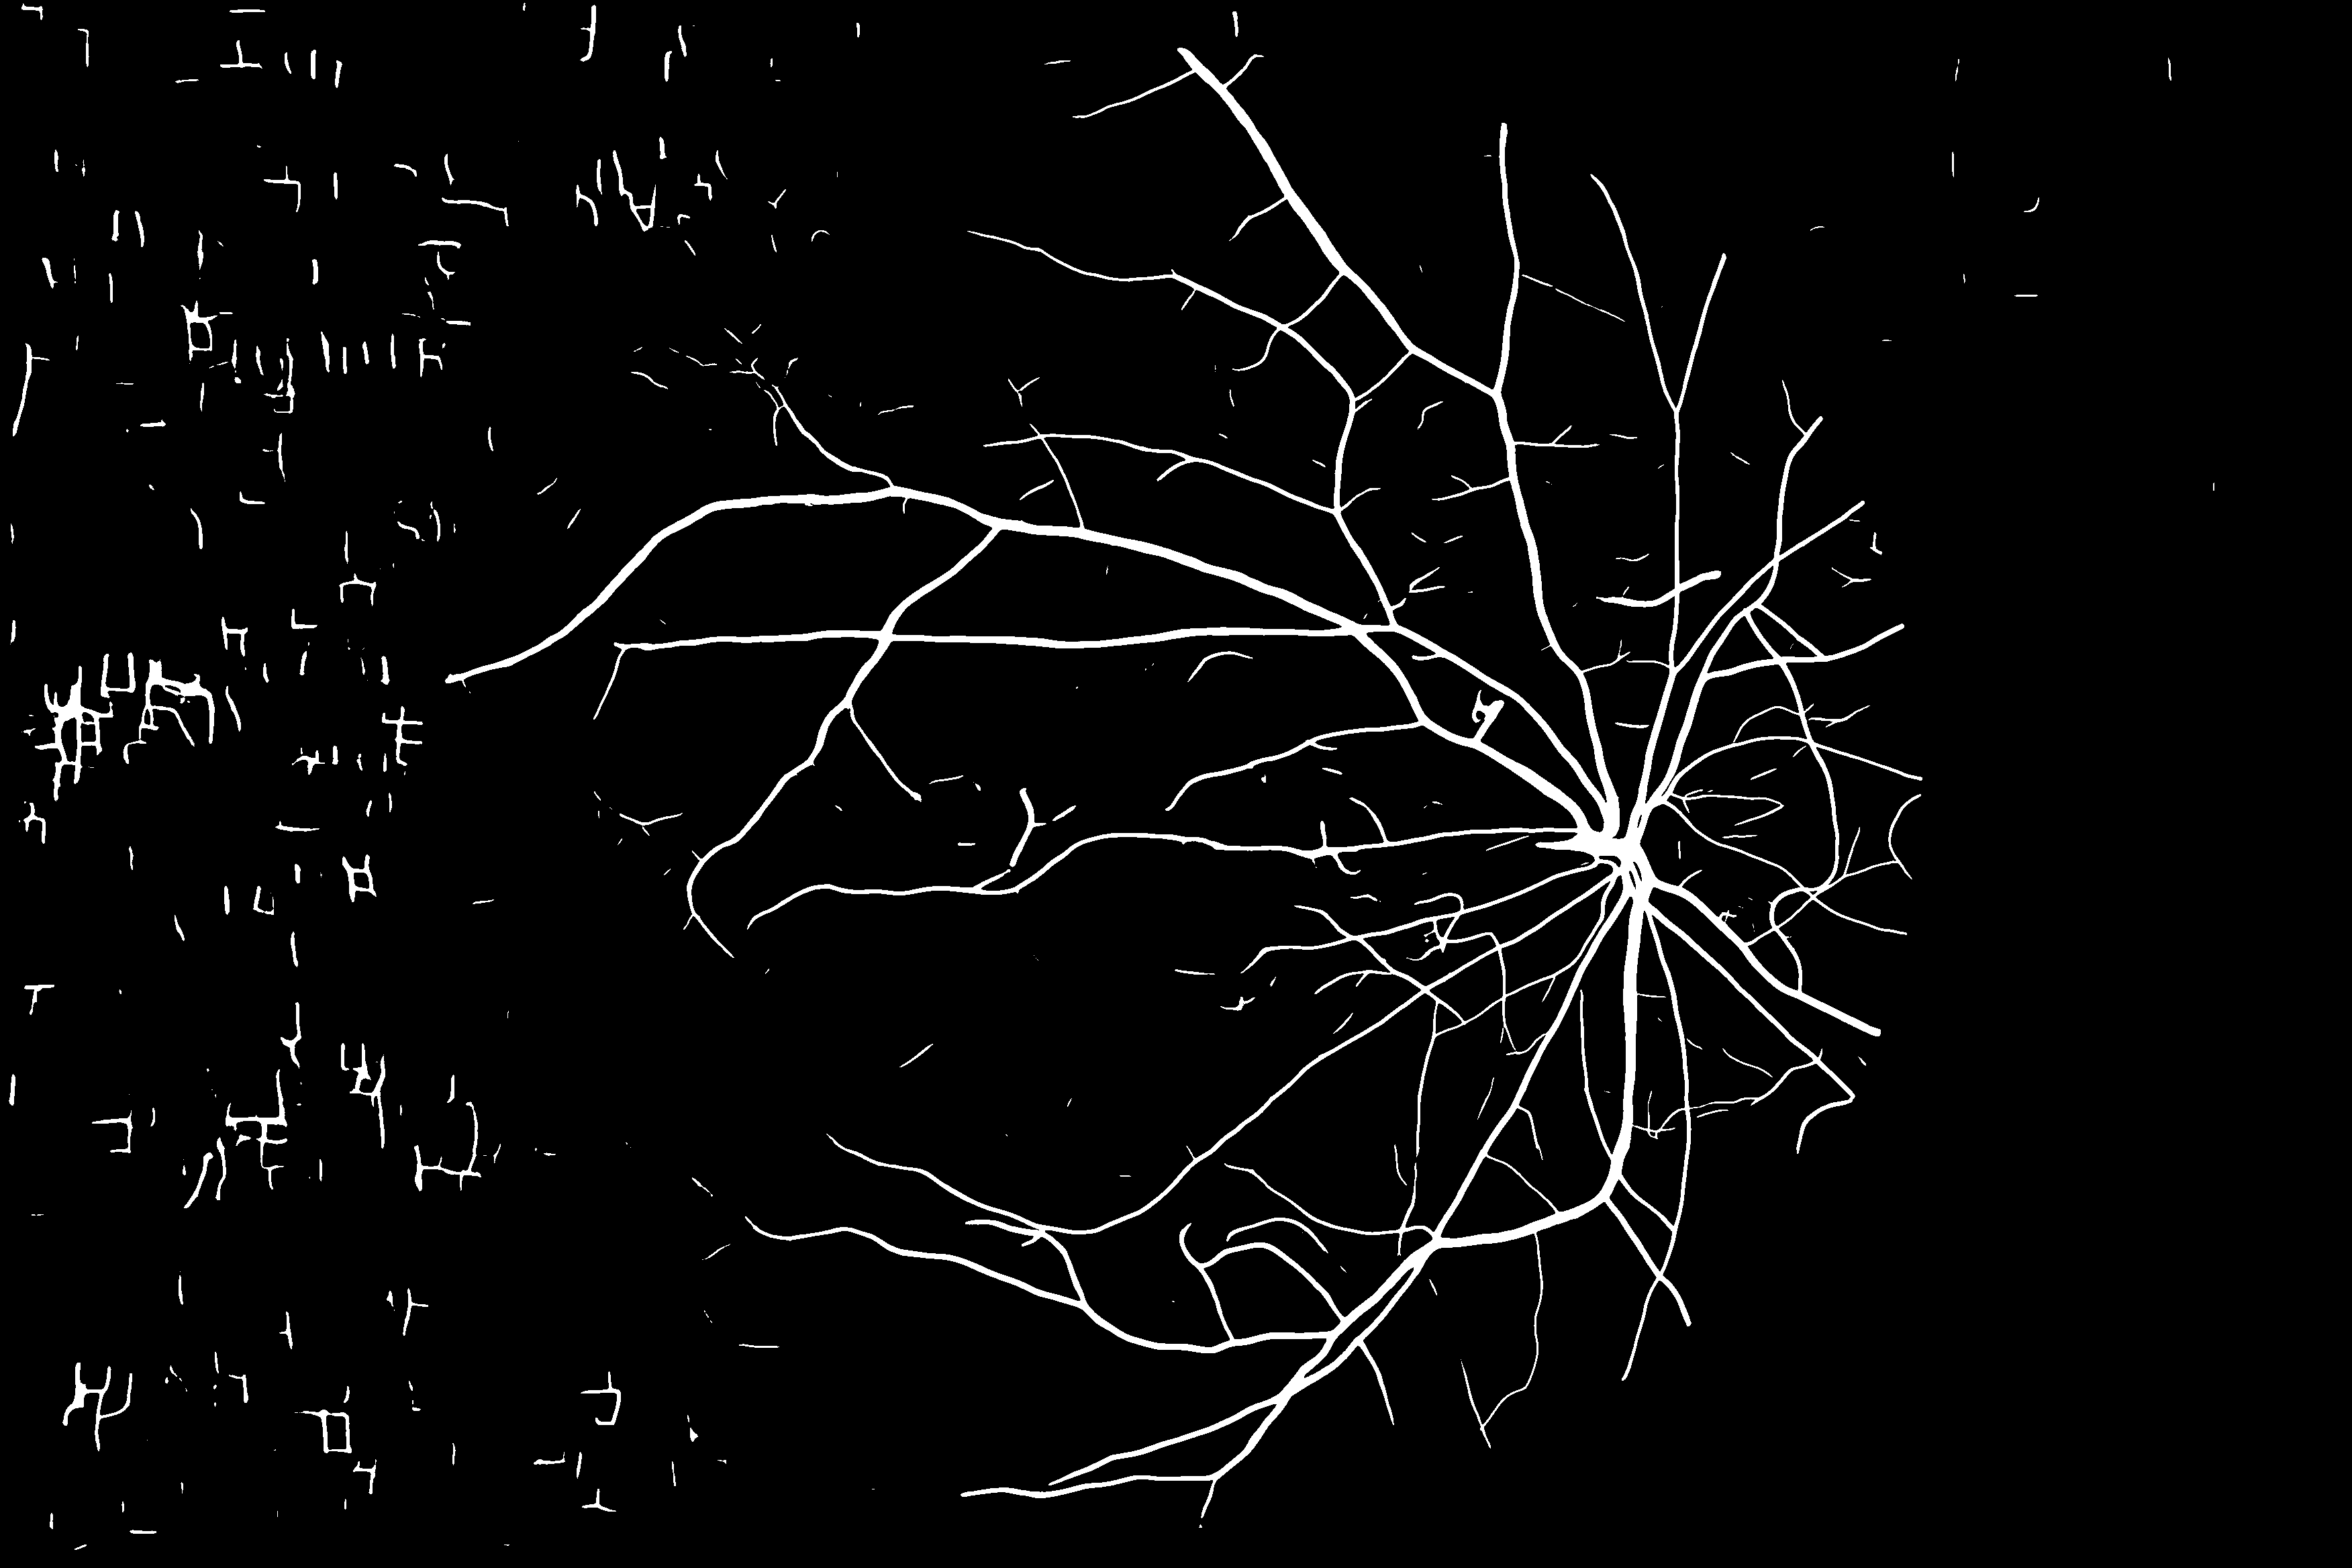
\includegraphics[width=\textwidth]{Pictures/nnUnet/Praxis/Task205-Augen-minimal-13-trainsamples/extra_Bilder/1170_right.png}
\end{minipage}%
\begin{minipage}{.5\textwidth}
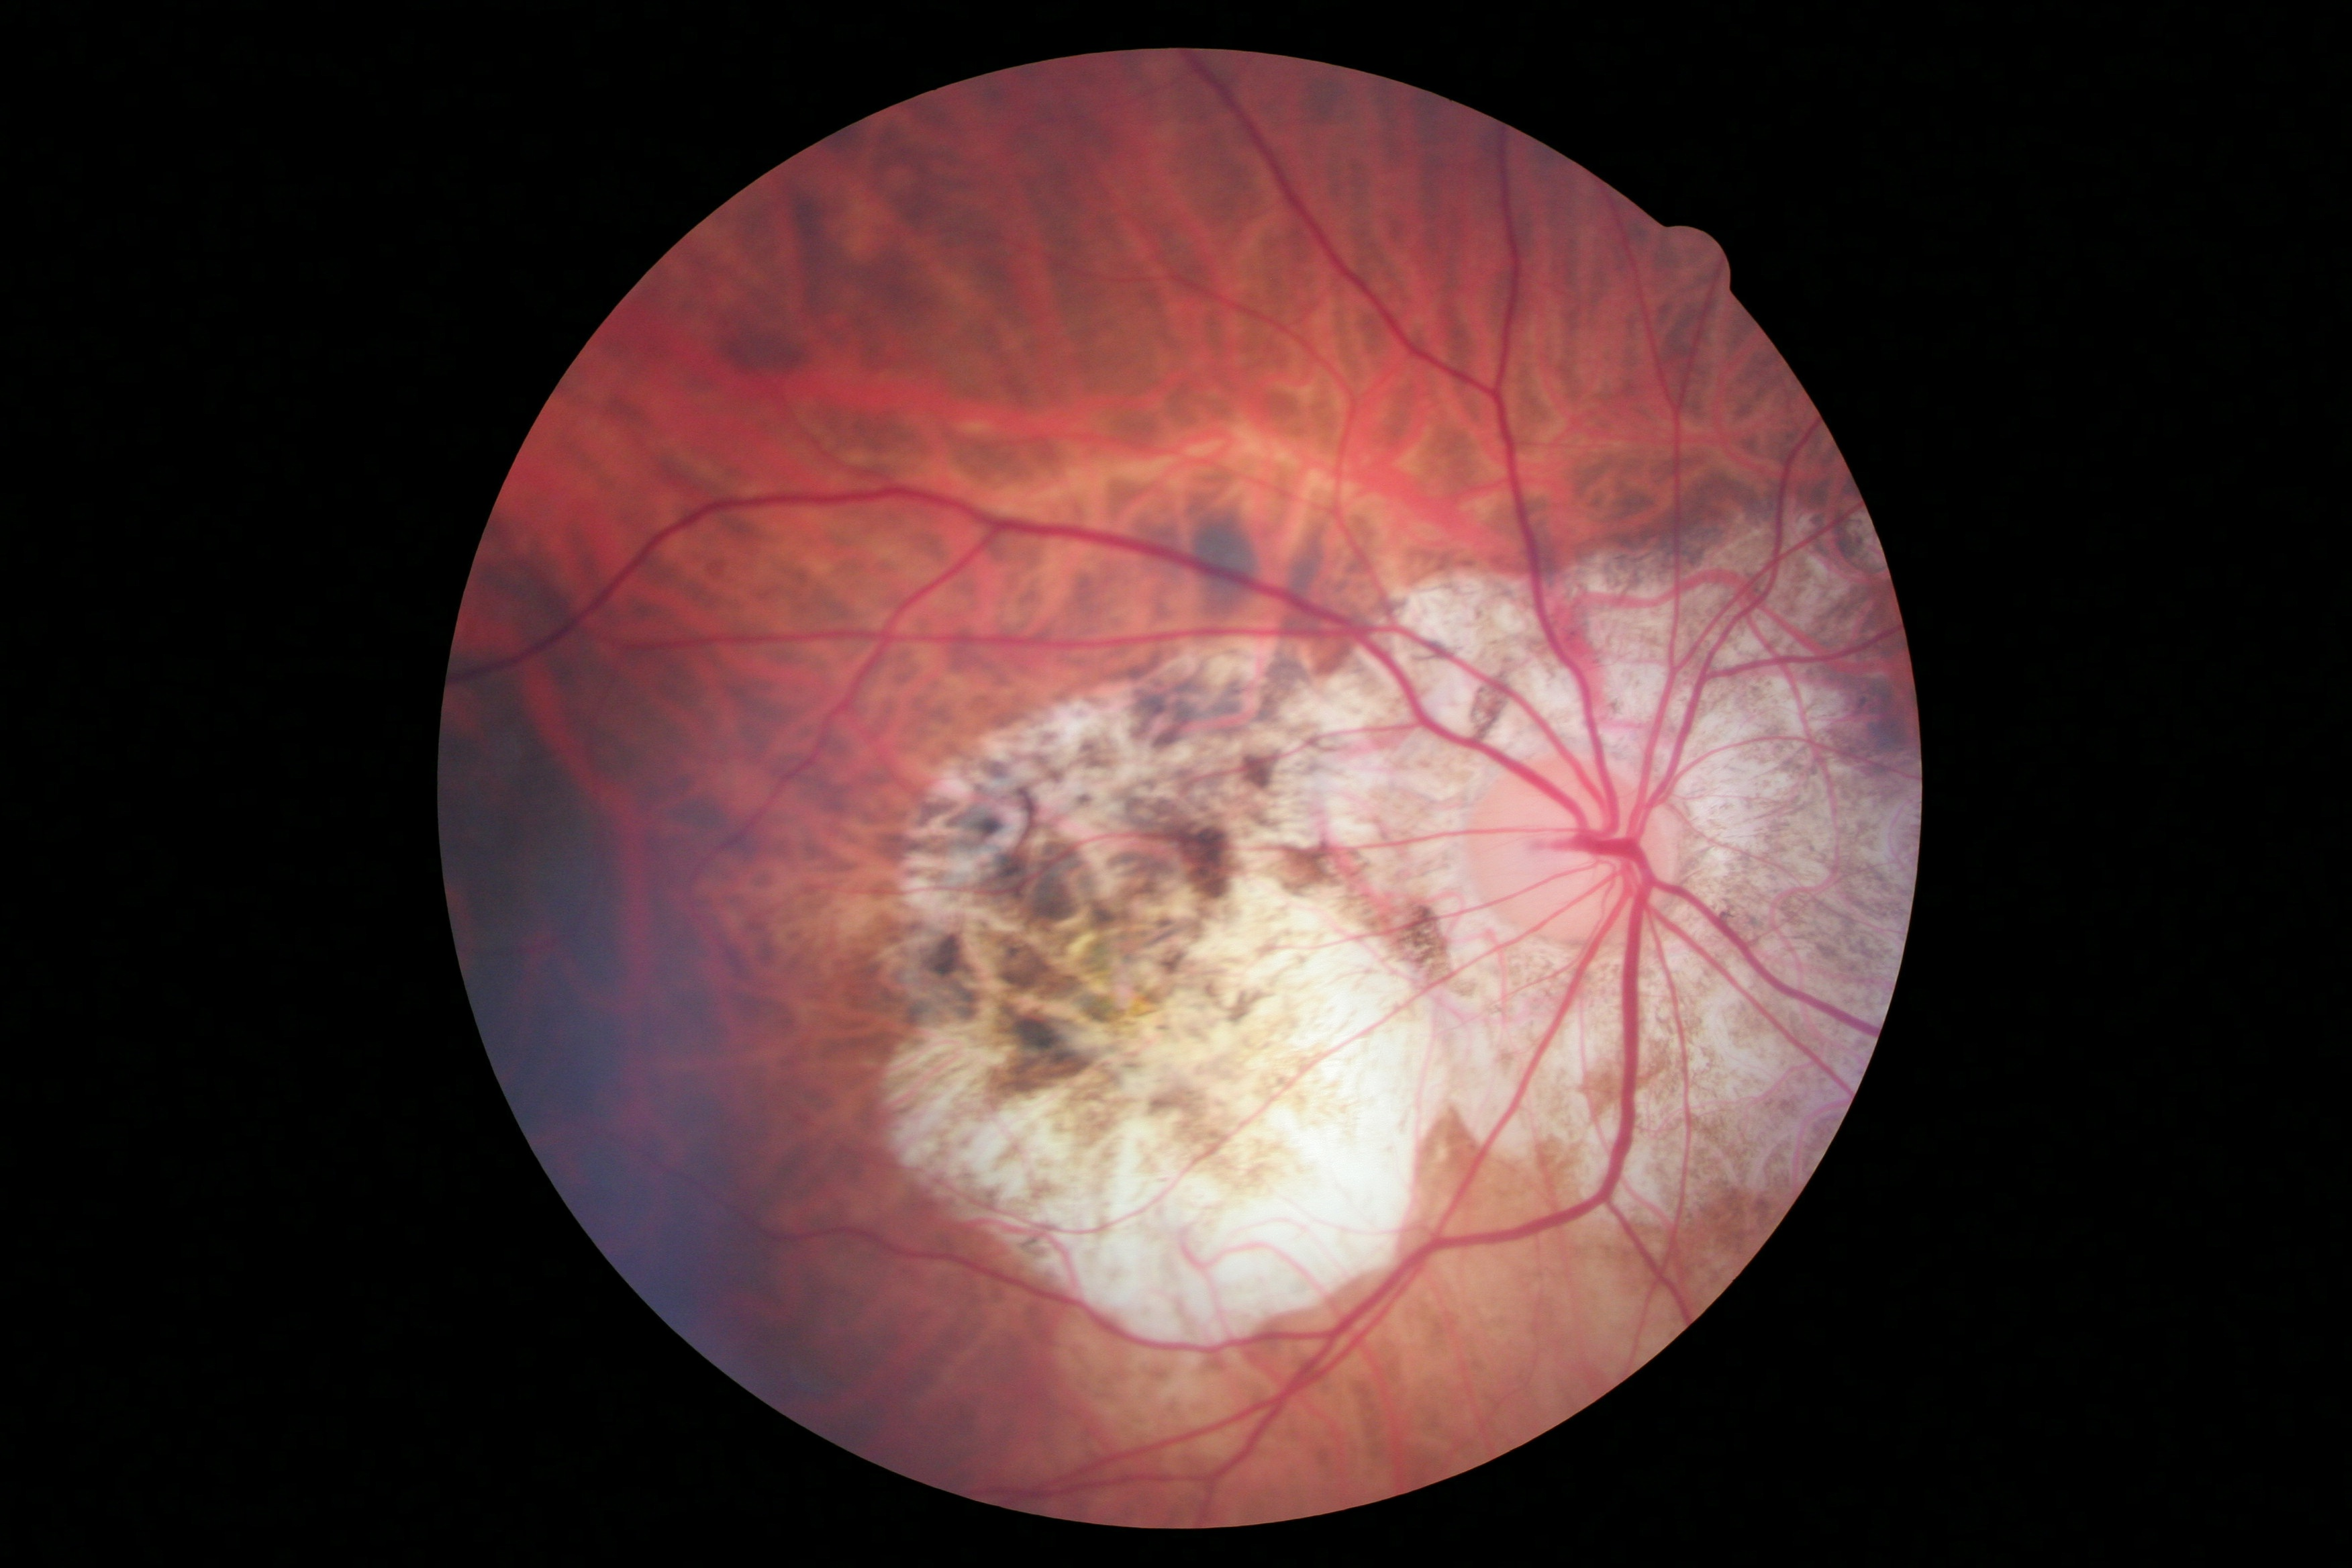
\includegraphics[width=\textwidth]{Pictures/nnUnet/Praxis/Task205-Augen-minimal-13-trainsamples/extra_Bilder/1170_right-original.jpeg}
\end{minipage}
\caption{Bild 1170\_right aus \cite{retina2dExtra} mit Wucherung im Hintergrund - Prediction und Original}
\label{pic:retinaExtraB}
\end{figure}




\subsection{CT-Datensatz}
\todo{Stimmt das so mit dem CT Datensatz?}
Da wir bisher nur eigene 2D-Datensätze in das Framework gegeben haben und es nur wenig öffentlich zugängliche 3D-Datensätze zur Segmentierung gibt, die nicht Teil der MSD-Challenge \cite{msdChallenge} sind, wurde uns ein Datensatz mit 19 Ganzkörper CT-Aufnahmen zur Verfügung gestellt \cite{ctDatensatz}, in denen Kalzium-Ablagerungen am Rand der Gefäße segmentiert werden sollen.
Auffällig ist hierbei, dass trotz der hohen Auflösung des Datensatzes (512x512 mit $\approx$ 400-600 Slices je Sample) nur \textit{sehr} wenig Pixel in der Segmentierung markiert sind. Bestenfalls sind $\approx$ 13000 Pixel im kompletten 3D Volumen bestehend aus 570 Slices mit je einer Auflösung von 512x512, was einem Anteil von \textit{maximal} 0,008\% entspricht. Außerdem gibt es auch Samples mit deutlich weniger oder gar keinen markierten Pixeln in der Ground-Truth Segmentierung (s. Abbildung \ref{pic:Haeuf_109}).

\begin{figure}[H]

\includesvg[width=\textwidth]{Pictures/nnUnet/Praxis/Task109-CT/Haeufigkeitsverteilung-109-CT}
\caption{Anteil von Objekt (Kalziumablagerung) je Sample mit Durchschnitt $\approx$ 0.002\%}
\label{pic:Haeuf_109}
\end{figure}


Dies erschwert das Training und könnte eine Begründung für die nicht sonderlich guten Ergebnisse sein.\\
Um den Datensatz in nnUNet zu geben mussten wir erst die zur Verfügung gestellten .nrrd (Ground-Truth) und .dcom (3D-CT-Scan) Dateien mit eigenen kleinen Pythonscripten \cite{autoMLGithub} in Nifti-Dateien umwandeln. Dabei sind wir auf sehr viele Probleme gestoßen und hatten erst kurz vor Ende des Projektseminars einigermaßen gute Ergebnisse. Zuerst hatten wir das Problem, dass beim Einlesen der .dcom und .nrrd Dateien die Drehung nicht intuitiv und nicht bei beiden gleich ist. Somit passte die Drehung der Ground-Truth Dateien nicht mehr zu den Original CT-Dateien, was aufgrund der geringen Häufigkeit an Pixeln in den Ground-Truth Daten und den mit dem Auge schwer ausfindig zu machenden zugehörigen Stellen im Original-Bild nicht direkt ersichtlich war.\\
Nachdem wir die Dateien passend gedreht haben und sie in allen Dimensionen übereinstimmten, konnten wir beim Training mit allen Netzvarianten keine sonderlich  guten Ergebnisse erzielen. Wir haben lange ausprobiert und gesucht, woran das liegen könnte, bis wir dann schließlich festgestellt haben, dass wir beim Konvertieren in Nifti-Dateien versehentlich den Wertebereich jedes Pixels von 16 Bit auf 8 Bit einschränken. Außerdem ist uns beim Trainieren erst nach zweimaligem Neustarten ohne Erfolg, mit sehr schlechten Ergebnissen bei genauerem Lesen des Papers aufgefallen, dass wir das Preprocessen in nnUNet bisher immer auf dem Login-Node des Clustercomputers Palma II durchgeführt haben, der keine Grafikkarte besitzt, um Wartezeiten in der Warteschlange zu vermeiden. Das Preprocessen ist aber abhängig von den zu dem Zeitpunkt zur Verfügung gestellten Ressourcen, insbesondere des verfügbaren GPU Speichers. Nachdem wir diesen Denkfehler behoben haben und den CT-Datensatz sowohl auf einer GPUv100 Karte preprocessed und trainiert haben, gelang es uns einigermaßen akzeptable Ergebnisse zu erzielen.



\begin{figure}[H]
\centering
\begin{minipage}{.5\textwidth}
\begin{subfigure}{\textwidth}
\centering
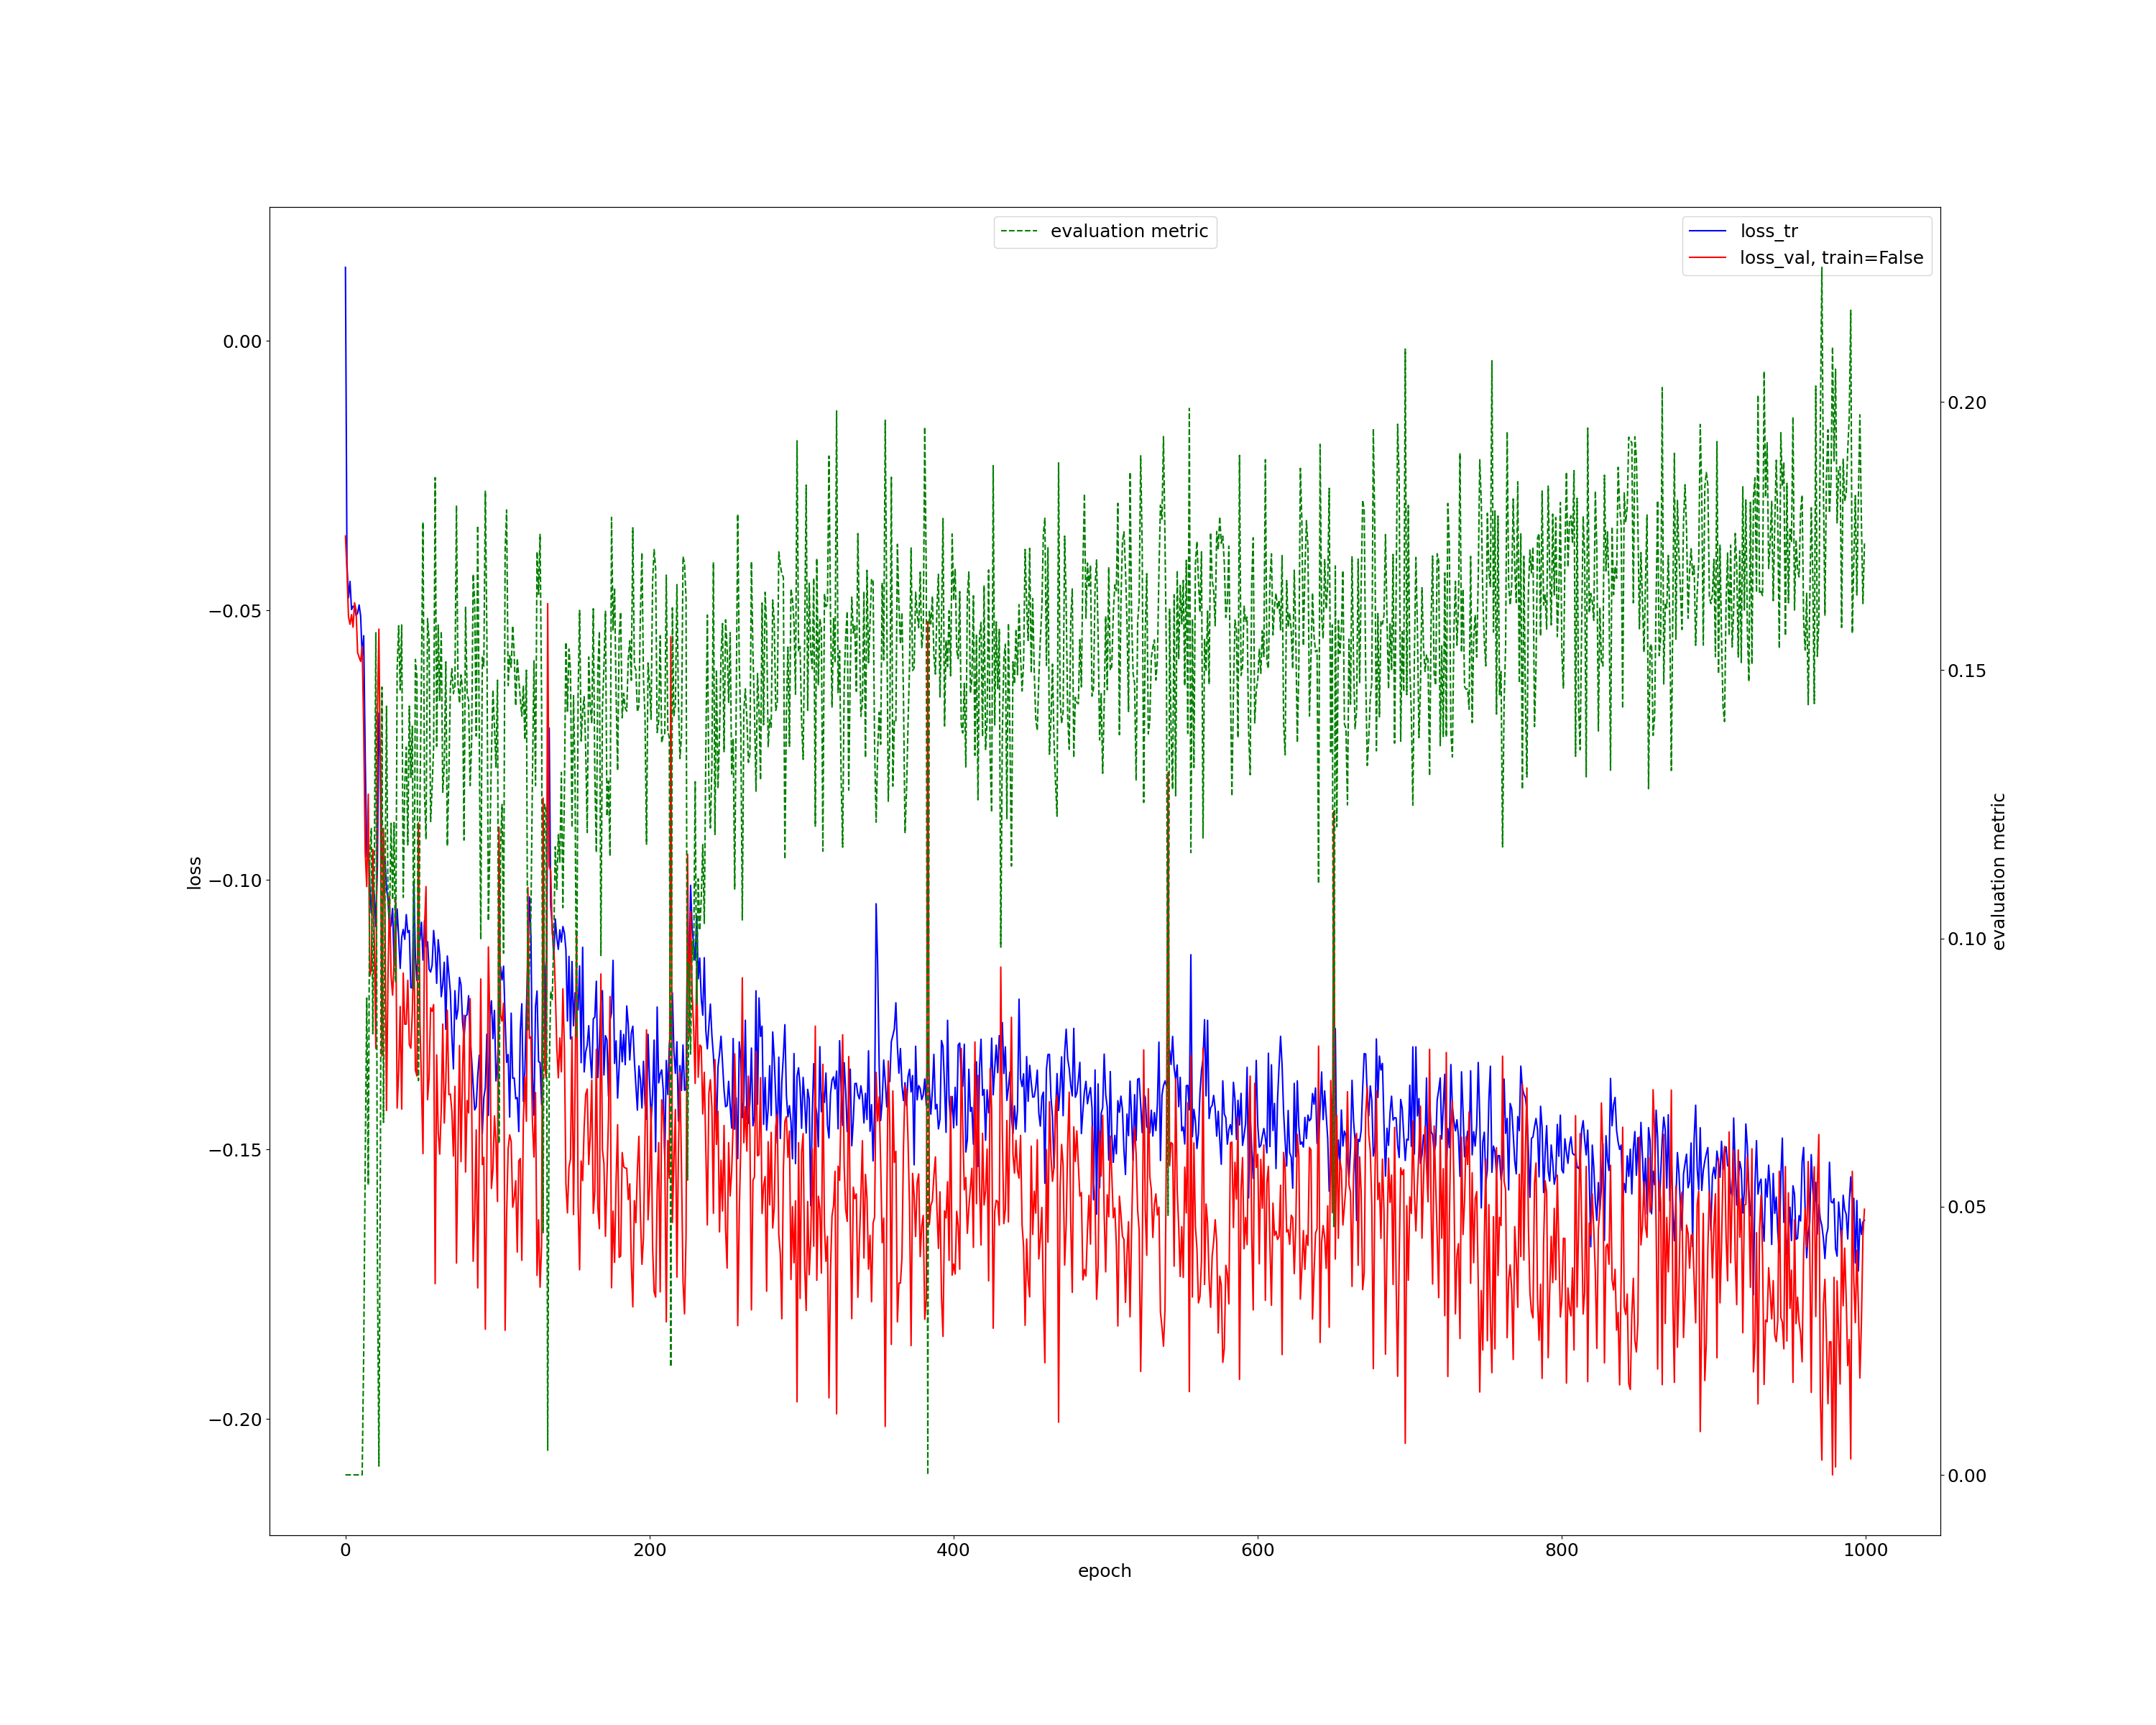
\includegraphics[width=\textwidth]{Pictures/nnUnet/Praxis/Task109-CT/progress_109-CT_2d.png}
\caption{2D Netz-Variante}
\label{pic:Prog_109-2d}
\end{subfigure}
\end{minipage}%
\begin{minipage}{.5\textwidth}
\begin{subfigure}{\textwidth}
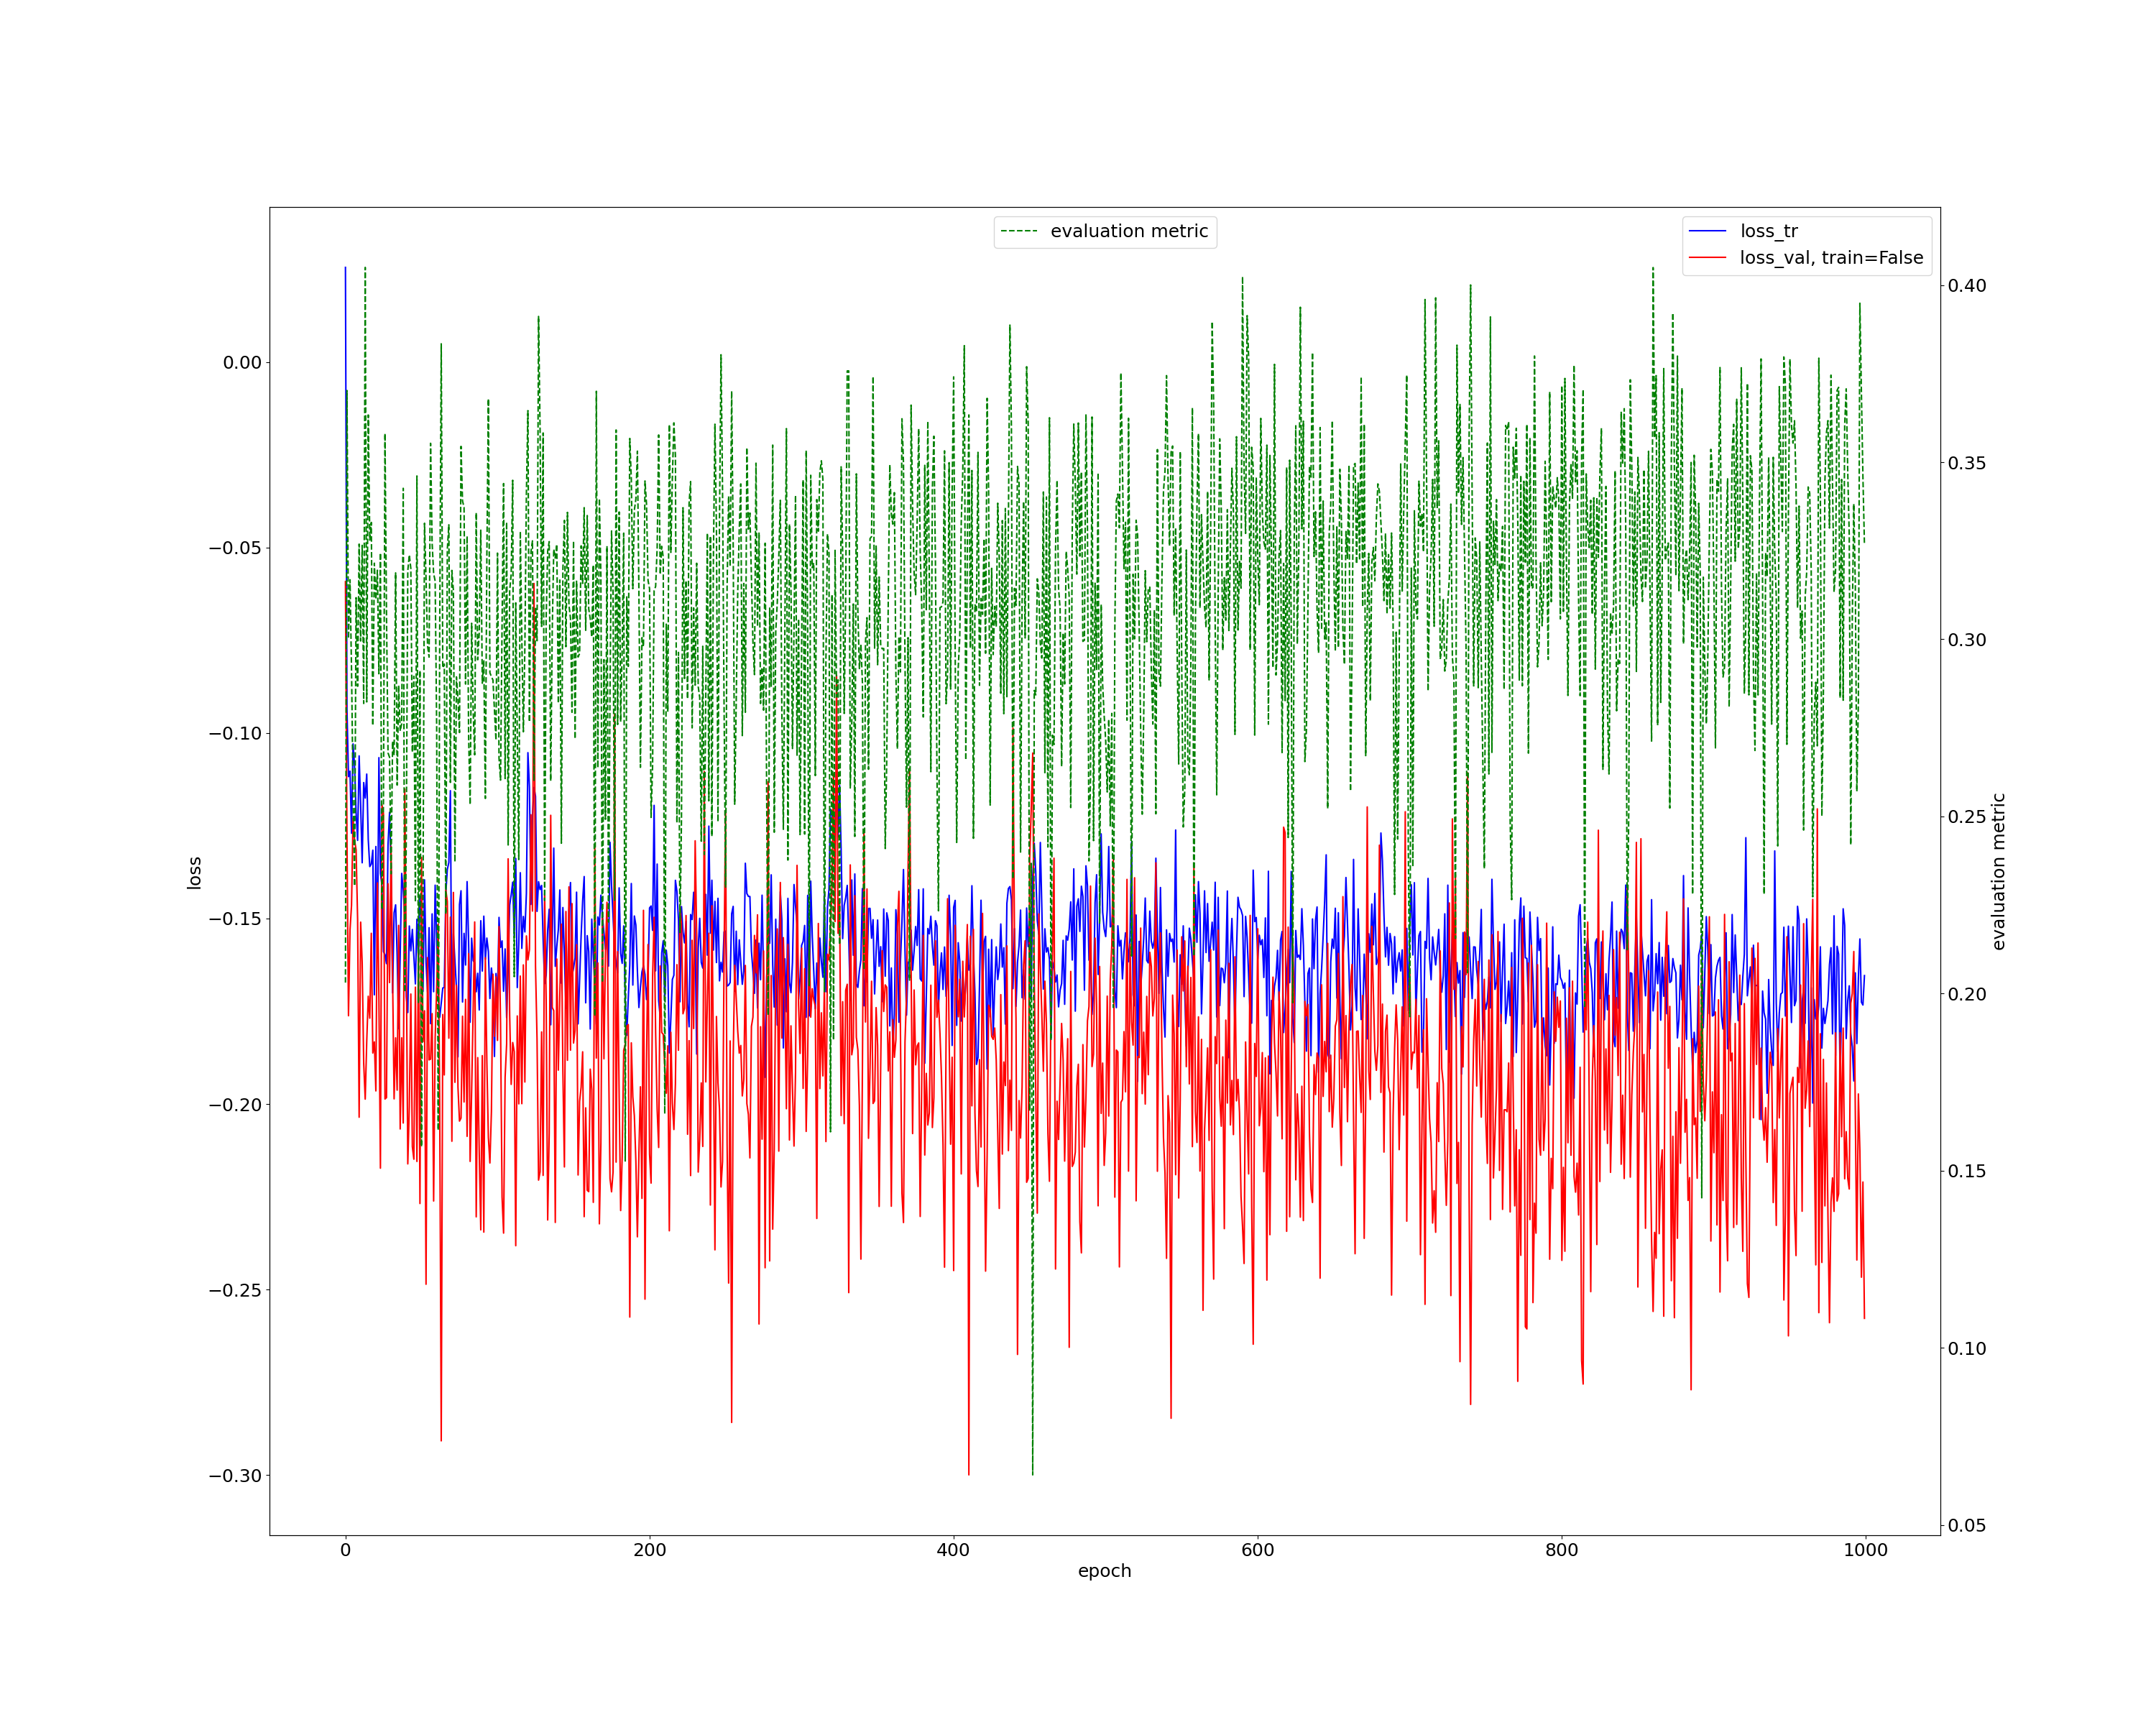
\includegraphics[width=\textwidth]{Pictures/nnUnet/Praxis/Task109-CT/progress_109-CT_3d_cascade_fullres.png}
\caption{3D\_cascade Netz-Variante}
\label{pic:Prog_109-cascade}
\end{subfigure}
\end{minipage}

\caption{Verlauf des Dice-Koeffizienten beim Training über 1000 Epochen}
\label{pic:Prog_109-A}
\end{figure}

Bei dem Training der 2D und 3D\_cascade Netz-Variante fällt auf, dass kaum eine Steigung vorhanden ist und die Ergebnisse mit einem Dice-Koeffizienten von $\approx 0.2$ bzw. $0.35$ gleichbleibend schlecht sind (s. Abbildung \ref{pic:Prog_109-A}).
Bei der 3D\_fullres Netz-Variante haben wir eine deutliche Steigung festgestellt, waren mit dem Ergebnis nach den standardmäßigen 1000 Epochen aber noch nicht zufrieden. Da die Steigung des Progress-Graphen (Abbildung \ref{pic:Prog_109-B}) auch bei Epoche 1000 noch relativ stark ist, haben wir das Training um weitere 1000 Epochen fortgesetzt und so insgesamt 2000 Epochen, also doppelt so lange wie die Standardeinstellung, trainieren lassen und konnten einen Dice-Koeffizienten von ca. 0.6 erreichen (s. Abbildung \ref{pic:Prog_109-B}).

\begin{figure}[H]
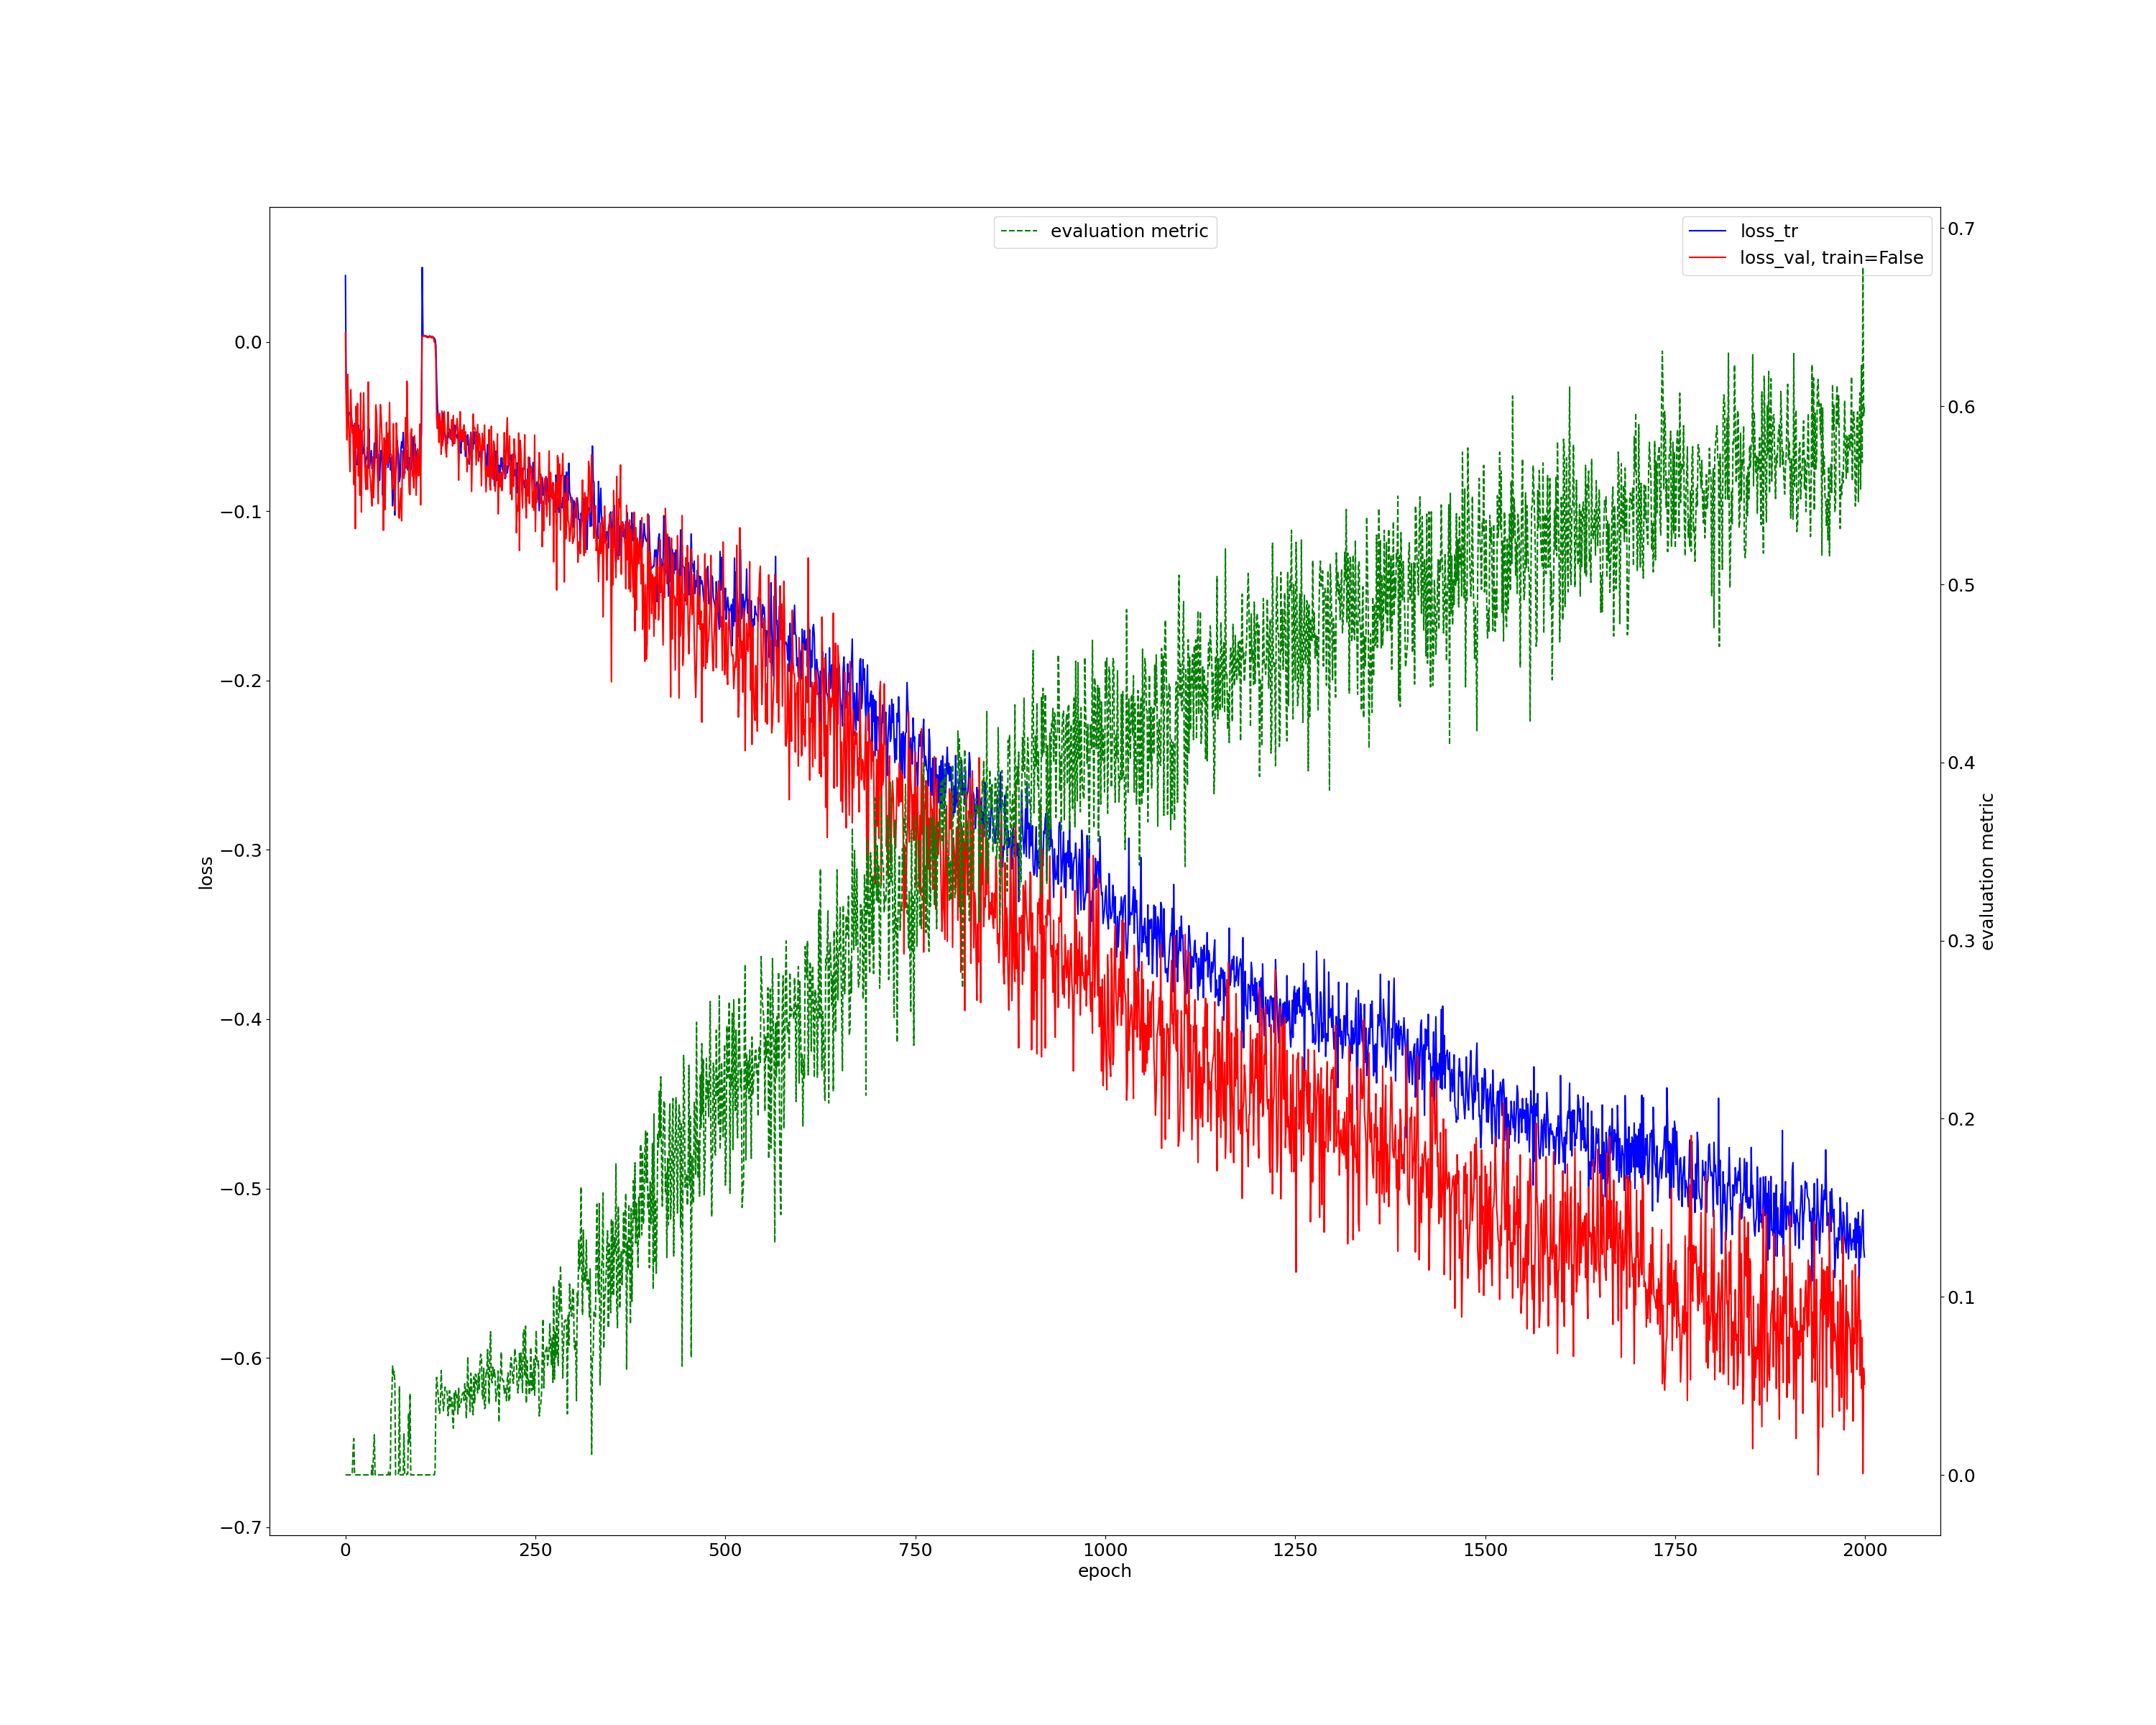
\includegraphics[width=\textwidth]{Pictures/nnUnet/Praxis/Task109-CT/progress_109-CT_3d_fullres.png}
\caption{Verlauf des Dice-Koeffizienten beim Training über 2000 Epochen mit 3D\_fullres}
\label{pic:Prog_109-B}
\end{figure}

Bei den Ergebnissen fällt auf, dass die Güte der Predictions bei 3D\_cascade stark streut und  nur in einem Fall sehr gut ist (s. Abbildung \ref{pic:Dice_109-cascade}). Die 2D Netz-Variante ist nicht zu gebrauchen (s. Abbildung \ref{pic:Dice_109-2d}). Dies liegt daran, dass dem 2D-Netz die Information über die Tiefe fehlt und nur die Slices einzeln für sich betrachtet werden.\\
Lediglich mit 3D\_fullres nach 2000 Epochen konnten wir einigermaßen akzeptable Ergebnisse erzielen (s. Abbildung \ref{pic:Dice_109-B}). Hierbei wurden Samples, die schon in Ground-Truth keinen einzigen markieren Pixel besitzen, ausgelassen, da dort kein Dice-Koeffizient berechnet werden kann.




\begin{figure}[H]
\centering
\begin{minipage}{.5\textwidth}
\begin{subfigure}{\textwidth}
\centering
\includesvg[width=\textwidth]{Pictures/nnUnet/Praxis/Task109-CT/Scatterplot-Dice-109-CT_2d}
\caption{2D Netz-Variante}
\label{pic:Dice_109-2d}
\end{subfigure}
\end{minipage}%
\begin{minipage}{.5\textwidth}
\begin{subfigure}{\textwidth}
\includesvg[width=\textwidth]{Pictures/nnUnet/Praxis/Task109-CT/Scatterplot-Dice-109-CT_3d_cascade}
\caption{3D\_cascade Netz-Variante}
\label{pic:Dice_109-cascade}
\end{subfigure}
\end{minipage}

\caption{Scatterplot der Dice-Koeffizienten je Sample in der 2D bzw 3D\_cascade Netz-Variante}
\label{pic:Dice_109-A}
\end{figure}

\begin{figure}[H]
\includesvg[width=\textwidth]{Pictures/nnUnet/Praxis/Task109-CT/Scatterplot-Dice-109-CT_3d_fullres}
\caption{Scatterplot der Dice-Koeffizienten je Sample in der 3D\_fullres Netz-Variante}
\label{pic:Dice_109-B}
\end{figure}



% Vis
%%%%%%%%%%%%%%%%%%%%%%%%%%% ORIG
\begin{figure}[H]
\begin{minipage}{0.3\textwidth}
\begin{subfigure}{\textwidth}
\centering
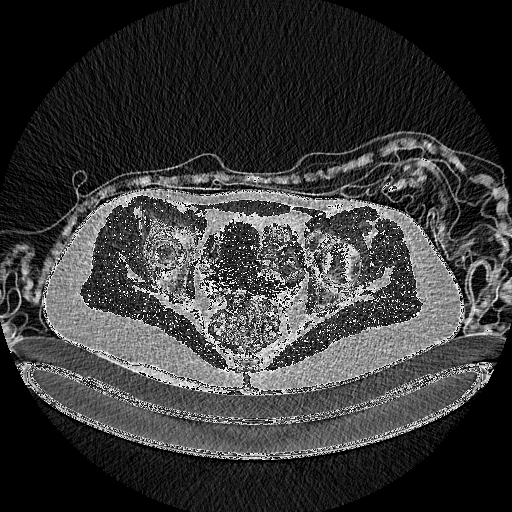
\includegraphics[width=\textwidth]{Pictures/nnUnet/Praxis/Task109-CT/samples/orig/orig_CT_003_0000-430.png}
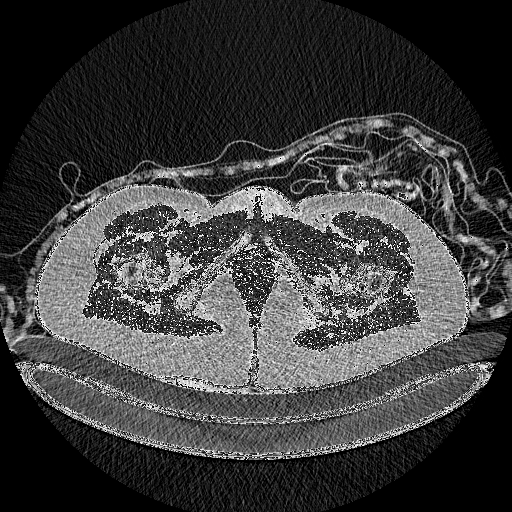
\includegraphics[width=\textwidth]{Pictures/nnUnet/Praxis/Task109-CT/samples/orig/orig_CT_003_0000-475.png}
\caption{Original CT Aufnahmen}
\end{subfigure}
\end{minipage}%
\hspace{3mm}
%%%%%%%%%%%%%%%%%%%%%%%%%%% GT
\begin{minipage}{0.3\textwidth}
\begin{subfigure}{\textwidth}
\centering
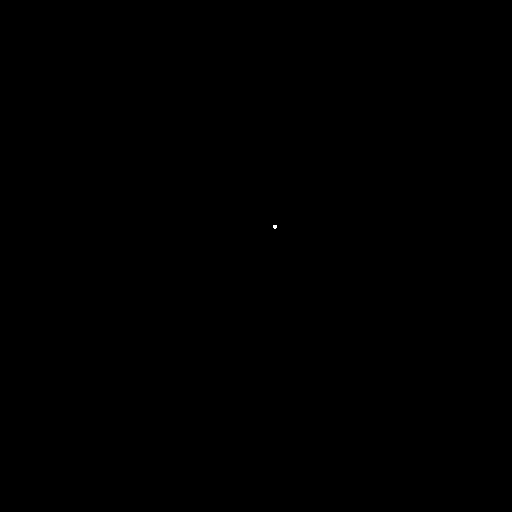
\includegraphics[width=\textwidth]{Pictures/nnUnet/Praxis/Task109-CT/samples/gt/gt_CT_003-430.png}
\centering
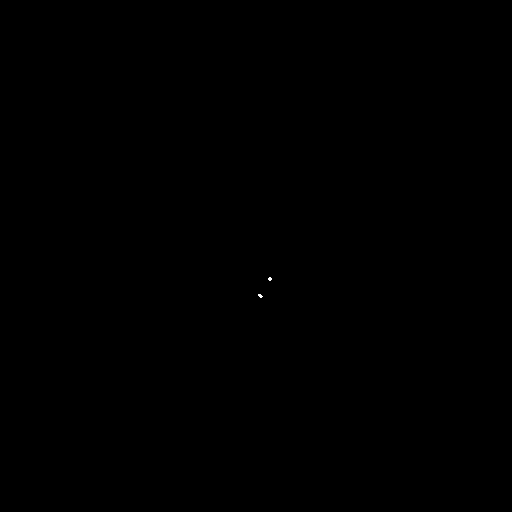
\includegraphics[width=\textwidth]{Pictures/nnUnet/Praxis/Task109-CT/samples/gt/gt_CT_003-475.png}
\caption{Ground-Truth}
\end{subfigure}
\end{minipage}%
\hspace{3mm}
%%%%%%%%%%%%%%%%%%%%%%%%%%% PRED
\begin{minipage}{0.3\textwidth}
\begin{subfigure}{\textwidth}
\centering
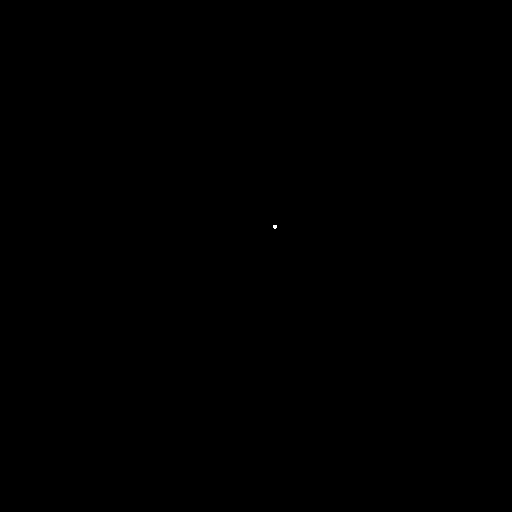
\includegraphics[width=\textwidth]{Pictures/nnUnet/Praxis/Task109-CT/samples/pred/pred_CT_003-430.png}

\includegraphics[width=\textwidth]{Pictures/nnUnet/Praxis/Task109-CT/samples/pred/pred_CT_003-475.png}
\caption{Predictions}
\end{subfigure}
\end{minipage}%
\caption{Visualisierung eines Samples (003)}
\label{pic:Vis_109}
\end{figure}

Bei der Visualisierung des zweitbesten Samples (Nummer 003, Dice=0,906) sieht man, wie wenig Pixel (insgesamt über alle Slices 1628 Stück) markiert sind und wie schwer zu erkennen die zugehörigen Stellen im Original CT-Bild sind (s. Abbildung \ref{pic:Vis_109}). In dem besten Sample (Nummer 018, Dice=1) wären es noch deutlich weniger Pixel gewesen (34 Stück).

\subsection{Pascal VOC2012}
\begin{figure}[H]

%\begin{subfigure}{\textwidth}
%\includesvg[width=\textwidth]{Pictures/nnUnet/Praxis/Task204-Pascal-VOC12-achtel-%testsplit/Haeufigkeitsverteilung-PascalVOC-Train}
%\caption{Trainsplit (10\% Stichprobe)}
%\label{pic:Haeuf-Train_204}
%\end{subfigure}


\begin{subfigure}{\textwidth}
\includesvg[width=\textwidth]{Pictures/nnUnet/Praxis/Task204-Pascal-VOC12-achtel-testsplit/Haeufigkeitsverteilung-PascalVOC-Train-zoomed}
\caption{Trainsplit vergrößert}
\label{pic:Haeuf-Train_204-zoom}
\end{subfigure}



%\begin{subfigure}{\textwidth}
%\includesvg[width=\textwidth]{Pictures/nnUnet/Praxis/Task204-Pascal-VOC12-achtel-%testsplit/Haeufigkeitsverteilung-PascalVOC-Test}
%\caption{Testsplit (50\% Stichprobe)}
%\label{pic:Haeuf-Test_204}
%\end{subfigure}


\begin{subfigure}{\textwidth}
\includesvg[width=\textwidth]{Pictures/nnUnet/Praxis/Task204-Pascal-VOC12-achtel-testsplit/Haeufigkeitsverteilung-PascalVOC-Test-zoomed}
\caption{Testsplit vergrößert}
\label{pic:Haeuf-Test_204-zoom}
\end{subfigure}
\caption{Durchschnittswerte für jede Klasse und ihre zugehörige Auftrittshäufigkeit im gesamten Datensatz}
\label{pic:Haeuf_204}
\end{figure}
\todo{Nicht-rangezoomte Version ist erstmal draußen. Unübersichtlich, groß, macht pdf langsam}

Nachdem wir bei den bisherigen 2D-Datensätzen nur Graustufen-Bilder mit einer Klasse (Larven \cite{larven}) und farbige Bilder mit einer Klasse (Retina 2D \cite{retina2d}) verwendet haben wollten wir auch noch einen 2D-Datensatz in Farbe mit mehreren Objekt-Klassen ausprobieren. Die Entscheidung fiel relativ schnell auf Pascal VOC2012 \cite{PascalVOCDatensatz}, da dieser sehr viele Klassen (20 Klassen + Background) und viele segmentierte Bilder (2856 Stück) in verschiedenen Formaten und Auflösungen zur Verfügung stellt und von vielen anderen Frameworks zum Vergleichen verwendet wird. Außerdem ist dieser Datensatz mit Fotografien nochmal wesentlich weiter von der \enquote{biomedical-domain} \cite{nnunetGithub2D-Daten}, für die das Framework eigentlich erstellt wurde, entfernt und dient somit als Test, wie robust das Framework mit verschiedenen Daten umgeht.\\\\
Um die Pascal-VOC 2012 Bilder in nnUNet zu geben mussten erst die Farbkodierungen in der Ground-Truth-Segmentierung in Indizes umgewandelt werden \cite{autoMLGithub}, da nnUNet bei 0=Background beginnend aufsteigende Integer für die Klassen erwartet aber in dem Pascal-Datensatz \cite{PascalVOCDatensatz} die Segmentierung zur besseren Erkennbarkeit farblich gekennzeichnet ist.\\
Außerdem mussten 57 Bilder, die nicht farbig sondern nur in Graustufen in Pascal-VOC 2012 \cite{PascalVOCDatensatz} vorhanden sind entfernt werden, da das Framework nicht mit einer variablen Anzahl an (Farb-) Kanälen umgehen kann.\\
Bei dem Datensatz ist auffällig, dass die Klassenhäufigkeiten sich untereinander unterscheiden und manche Klassen wesentlich häufiger auftreten als andere. Im Train- und im Testsplit ist diese Unausgeglichenheit jedoch ähnlich (s. Abbildung \ref{pic:Haeuf_204}).

Um die Gesamt-Performance auf diesem Datensatz auszuwerten mussten wir erstmalig über mehrere Klassen einen Durchschnitt bilden. Naiv könnte man die Dice-Koeffizienten jeder Klasse addieren und am Ende durch die Anzahl der Klassen teilen. Dies hätte jedoch die Folge, dass gute bzw. schlechte Klassen, die sehr selten vorkommen, das Endergebnis unverhältnismäßig nach oben bzw. unten ziehen. Wir haben uns für eine Gewichtung der Form
\[\text{average} = \frac{\sum_i{d_i * n_i}}{\sum_i{n_i}}\]
mit $d_i$: Dice-Koeffizient eines Samples für Klasse $i$\\
$n_i$: Anzahl zu Klasse $i$ gehöriger Pixel im Ground-Truth des Samples.\\
Diese Formel kann auch auf die Durchschnittswerte, die automatisch vom Framework je Klasse generiert werden, angewandt werden um einen Durchschnittswert über alle Klassen hinweg zu bilden.\\\\
Das Training verlief gut und es konnten, wie von den anderen Datensätzen gewohnt, relativ schnell gute Ergebnisse auf dem Trainsplit bzw. im Progress-Graph verzeichnet werden. Im Testsplit sind die Ergebnisse jedoch weit von denen aus dem Trainsplit entfernt.
Dies zeigt unserer Meinung nach die Grenzen dieses Frameworks auf, da es bisher sehr gut mit regelmäßigen Mustern und Strukturen wie z.B. bei den Larven oder den Retina Adern umgehen konnte, jedoch jetzt bei Fotografien aus verschiedenen Blickwinkeln mit Objekten von Klassen in verschiedenen Größen, die sich zudem noch sehr stark ähneln (z.B. Schaf und Hund) schlecht abschneidet. Außerdem ist auffällig, dass bestimmte Klassen wesentlich schlechter auf dem Testsplit sind als andere (s. Abbildung \ref{pic:Prog_204} und \ref{pic:Dice_204}).

\begin{figure}[H]
\centering
\begin{subfigure}{\textwidth}
\centering
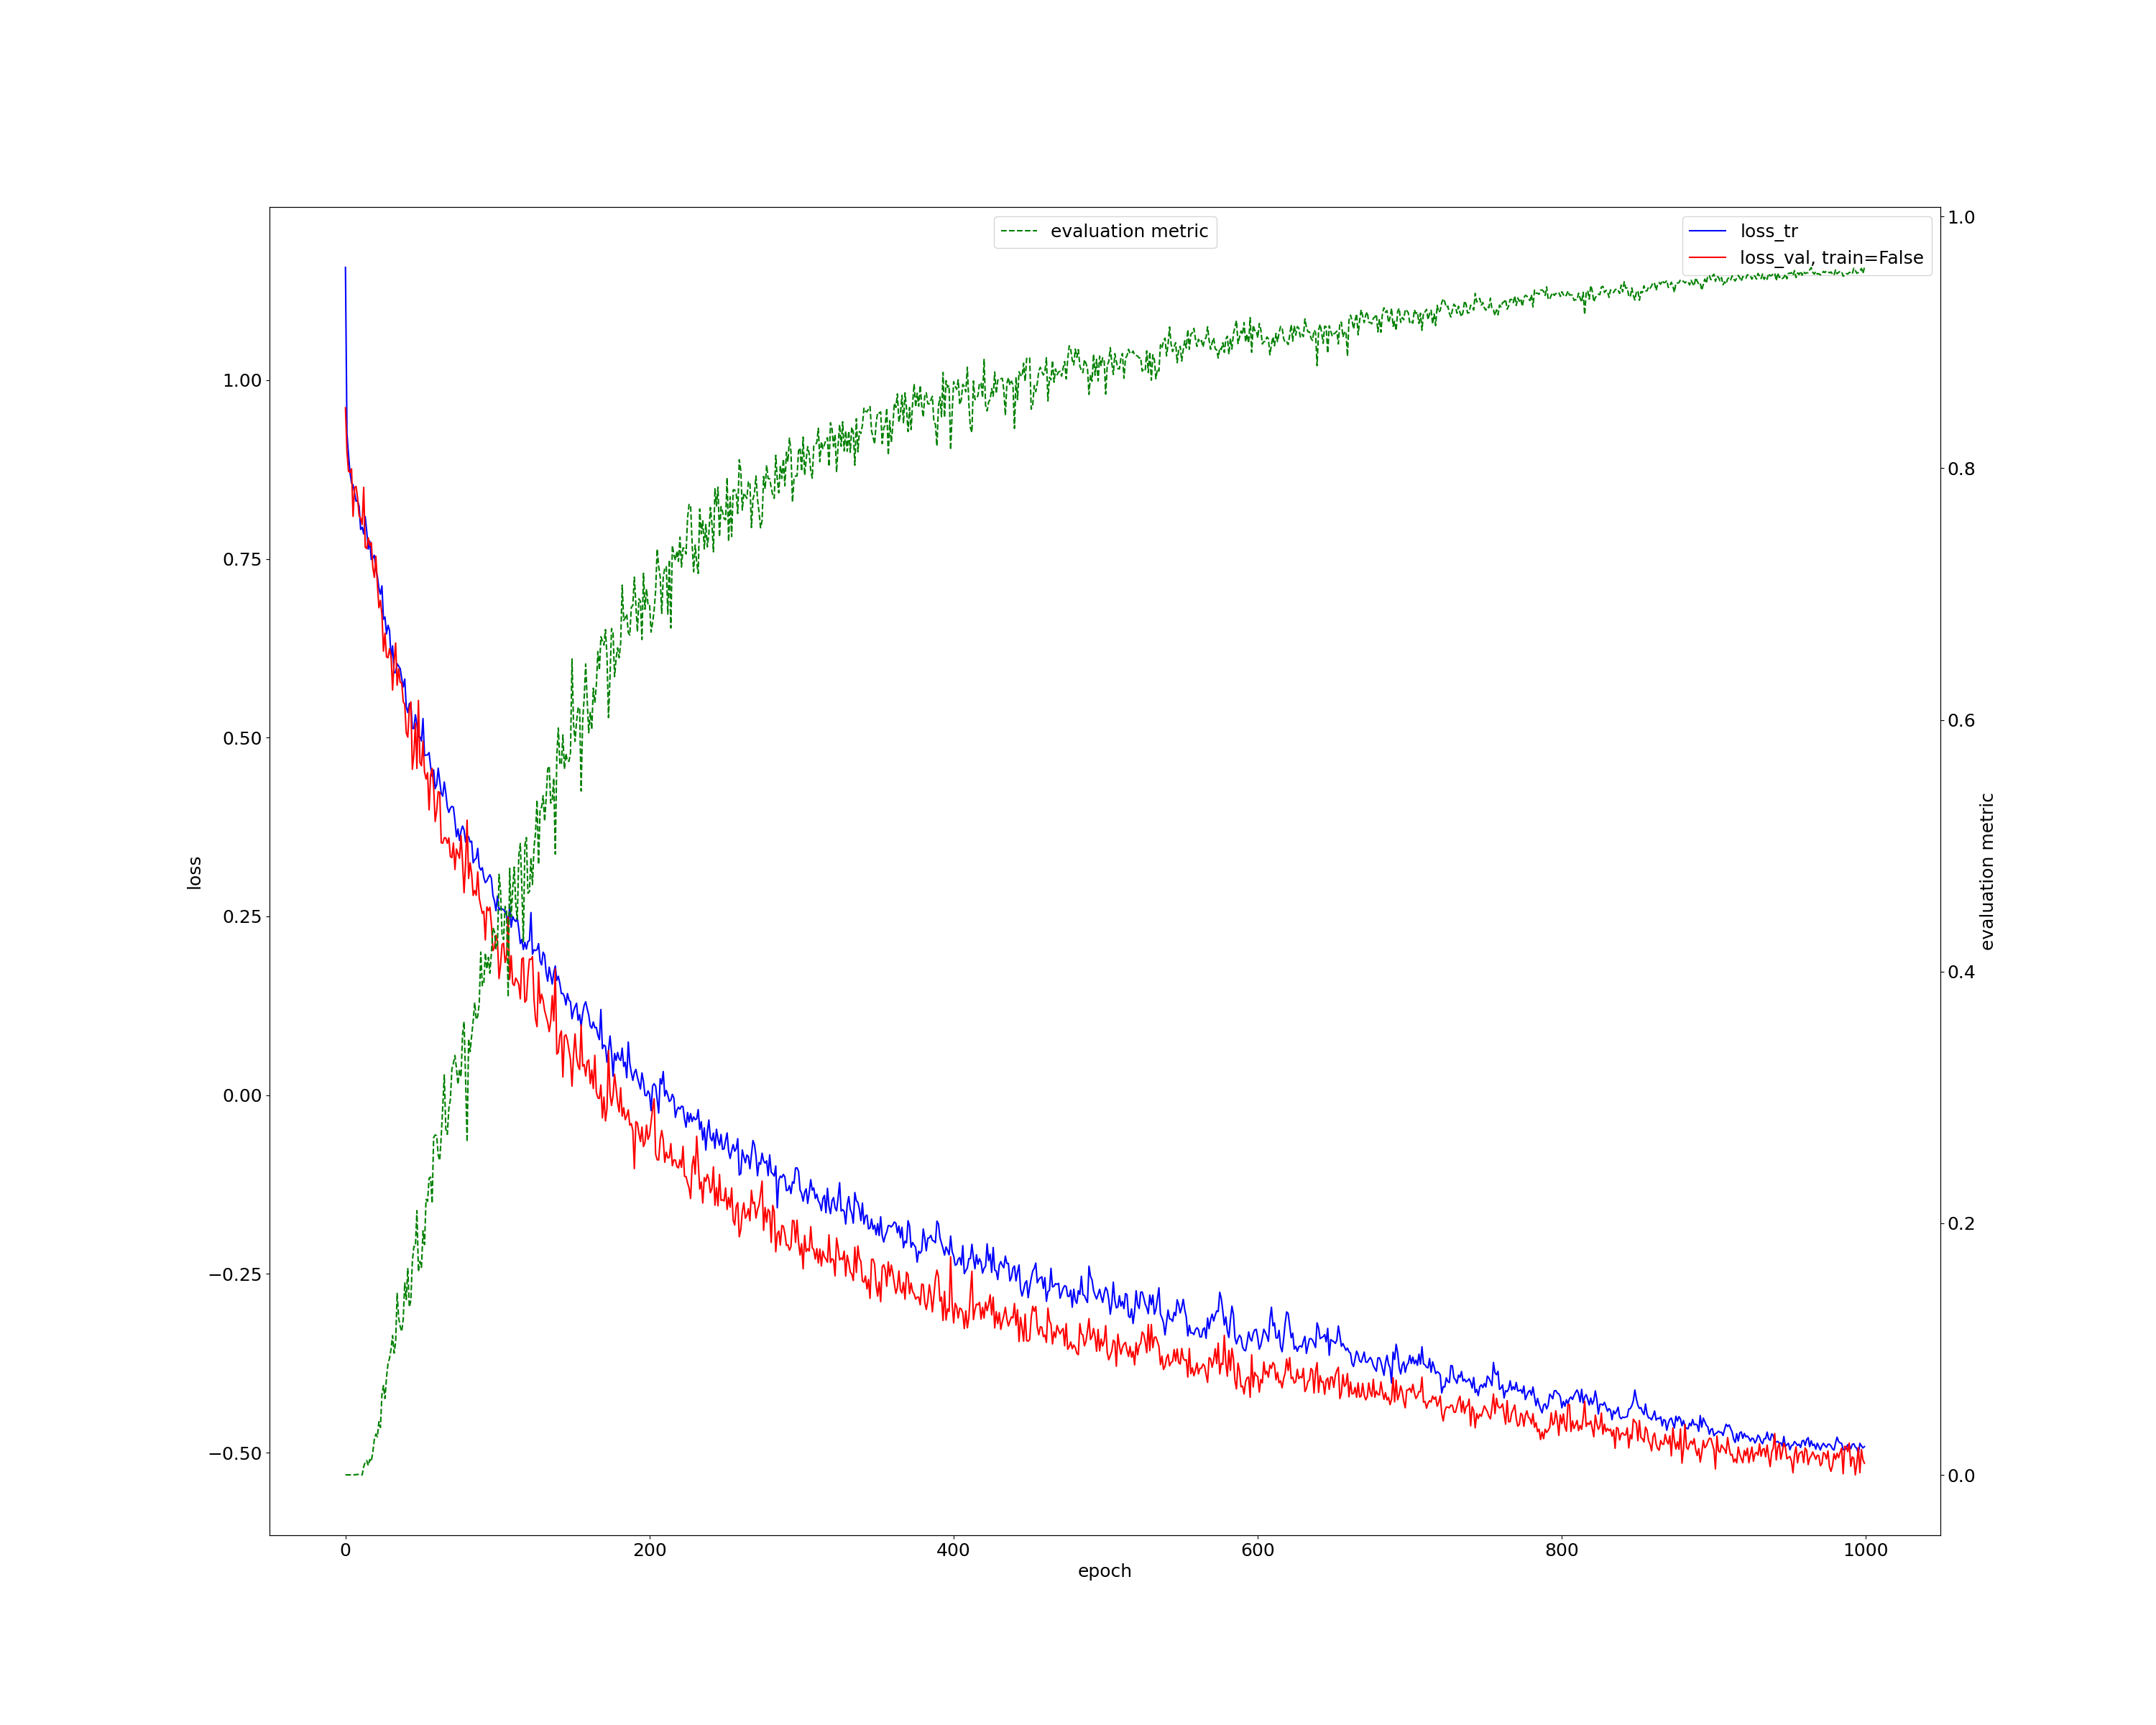
\includegraphics[width=.6\textwidth]{Pictures/nnUnet/Praxis/Task204-Pascal-VOC12-achtel-testsplit/progress_204-Pascal-VOC12-achtel-testsplit.png}
\caption{Verlauf des Dice-Koeffizienten beim Training über 1000 Epochen}
\label{pic:Prog_204}
\end{subfigure}

\begin{subfigure}{\textwidth}
\includesvg[width=\textwidth]{Pictures/nnUnet/Praxis/Task204-Pascal-VOC12-achtel-testsplit/Scatterplot-Dice}
\caption{Scatterplot der Dice-Koeffizienten je Sample für Train- und Testsplit}
\label{pic:Dice_204}
\end{subfigure}

\caption{Dice-Koeffizienten zum PascalVOC 2012 \cite{PascalVOCDatensatz} Datensatz mit $\frac{7}{8}$ Trainsplit und $\frac{1}{8}$ Testsplit}
\end{figure}


Bei der Visualisierung fällt auf, dass auf dem Trainsplit die meisten Objekte grob erkannt werden, nur bei feineren Strukturen (z.B. dem kleinen Fahrrad) wird ungenau segmentiert. Ansonsten sind keine groben Fehler vorhanden und es werden keine Klassen verwechselt (s. Abbildung \ref{pic:Vis-Train_204}).\\
Auf dem Testsplit hingegen sieht man, dass ähnlich aussehende Klassen wie z.B. Person, Schaf, Kuh und Hund häufig verwechselt werden, aber im Median eine ziemlich solide Performance gegeben ist (s. Abbildung \ref{pic:Vis-Test_204}).

\begin{figure}[H]
\centering
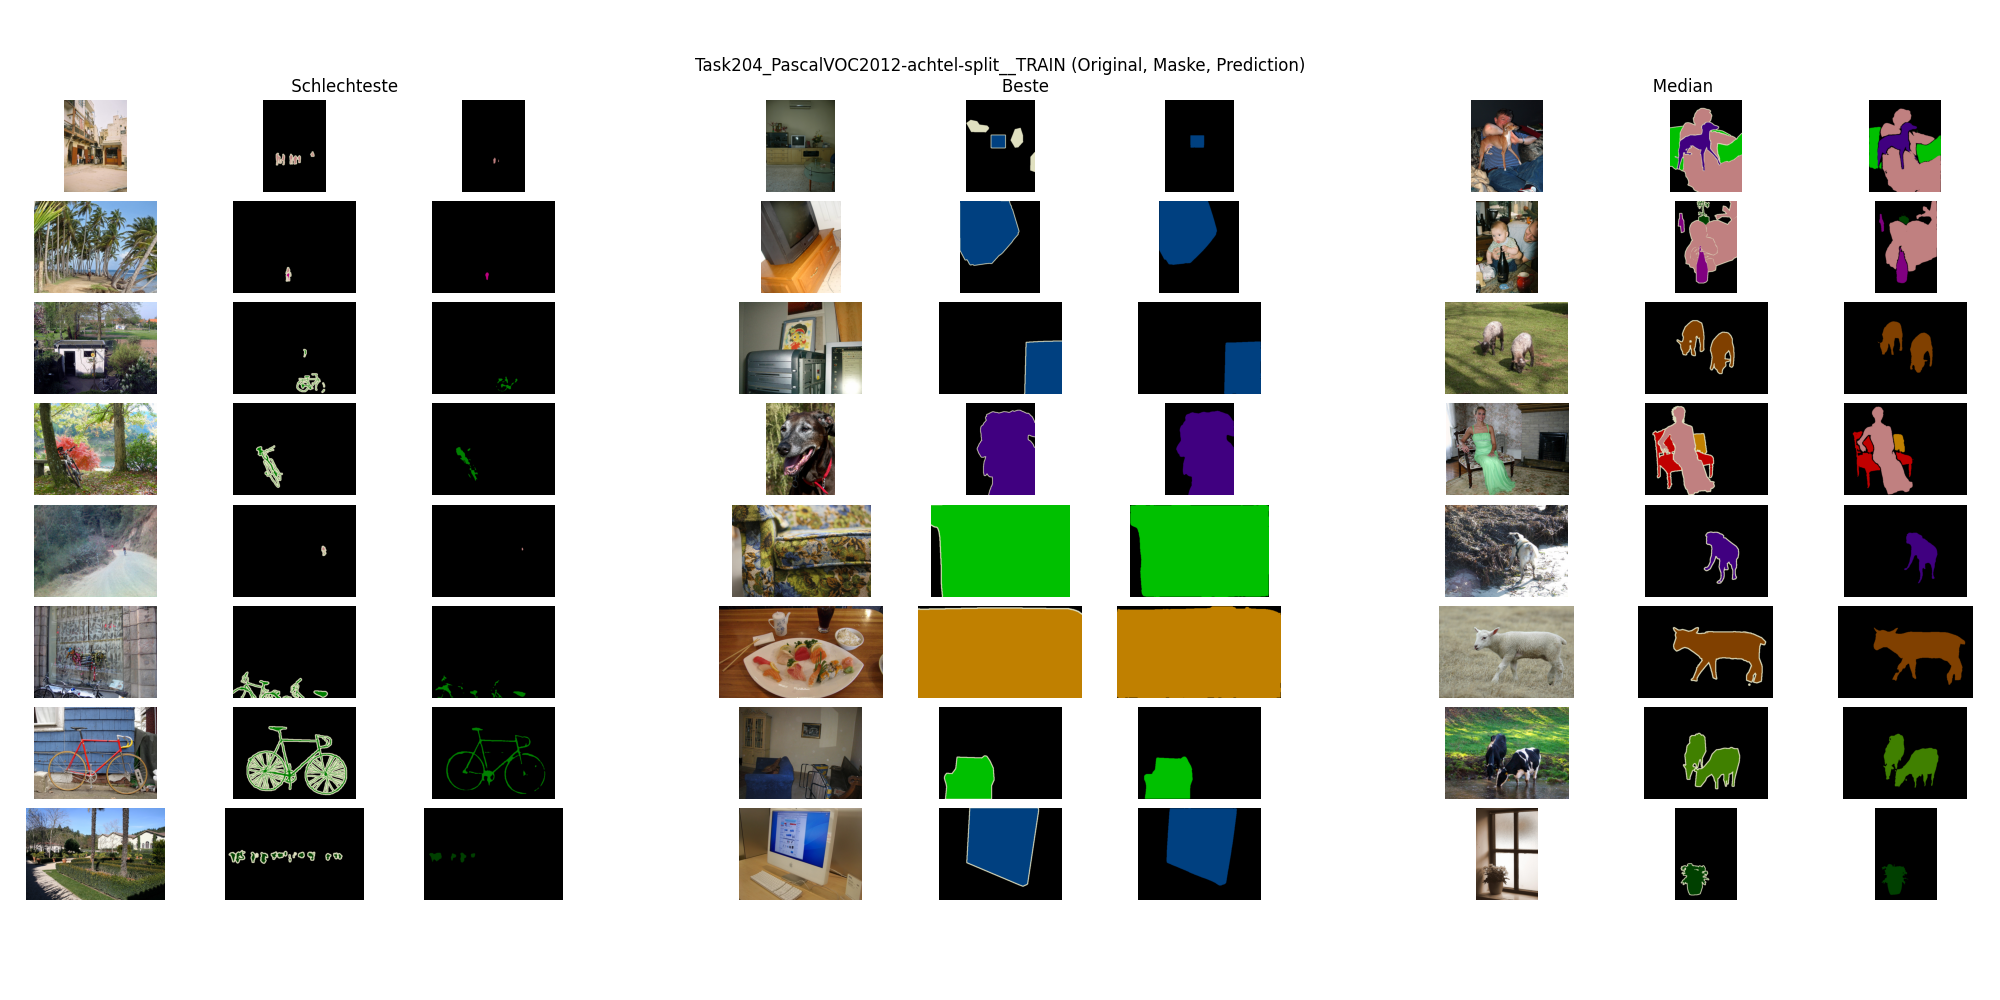
\includegraphics[height=0.35\textheight, width=\textwidth]{Pictures/nnUnet/Praxis/Task204-Pascal-VOC12-achtel-testsplit/Vis-Train.png}
\caption{Visualisierung des Trainsplits auf dem PascalVOC 12 \cite{PascalVOCDatensatz} Datensatz (links: schlechteste Ergebnisse, mitte: beste Ergebnisse, rechts: Ergebnisse im Median; jeweils Original, Ground-Truth und Prediction)}
\label{pic:Vis-Train_204}
\end{figure}


\begin{figure}[H]
\centering
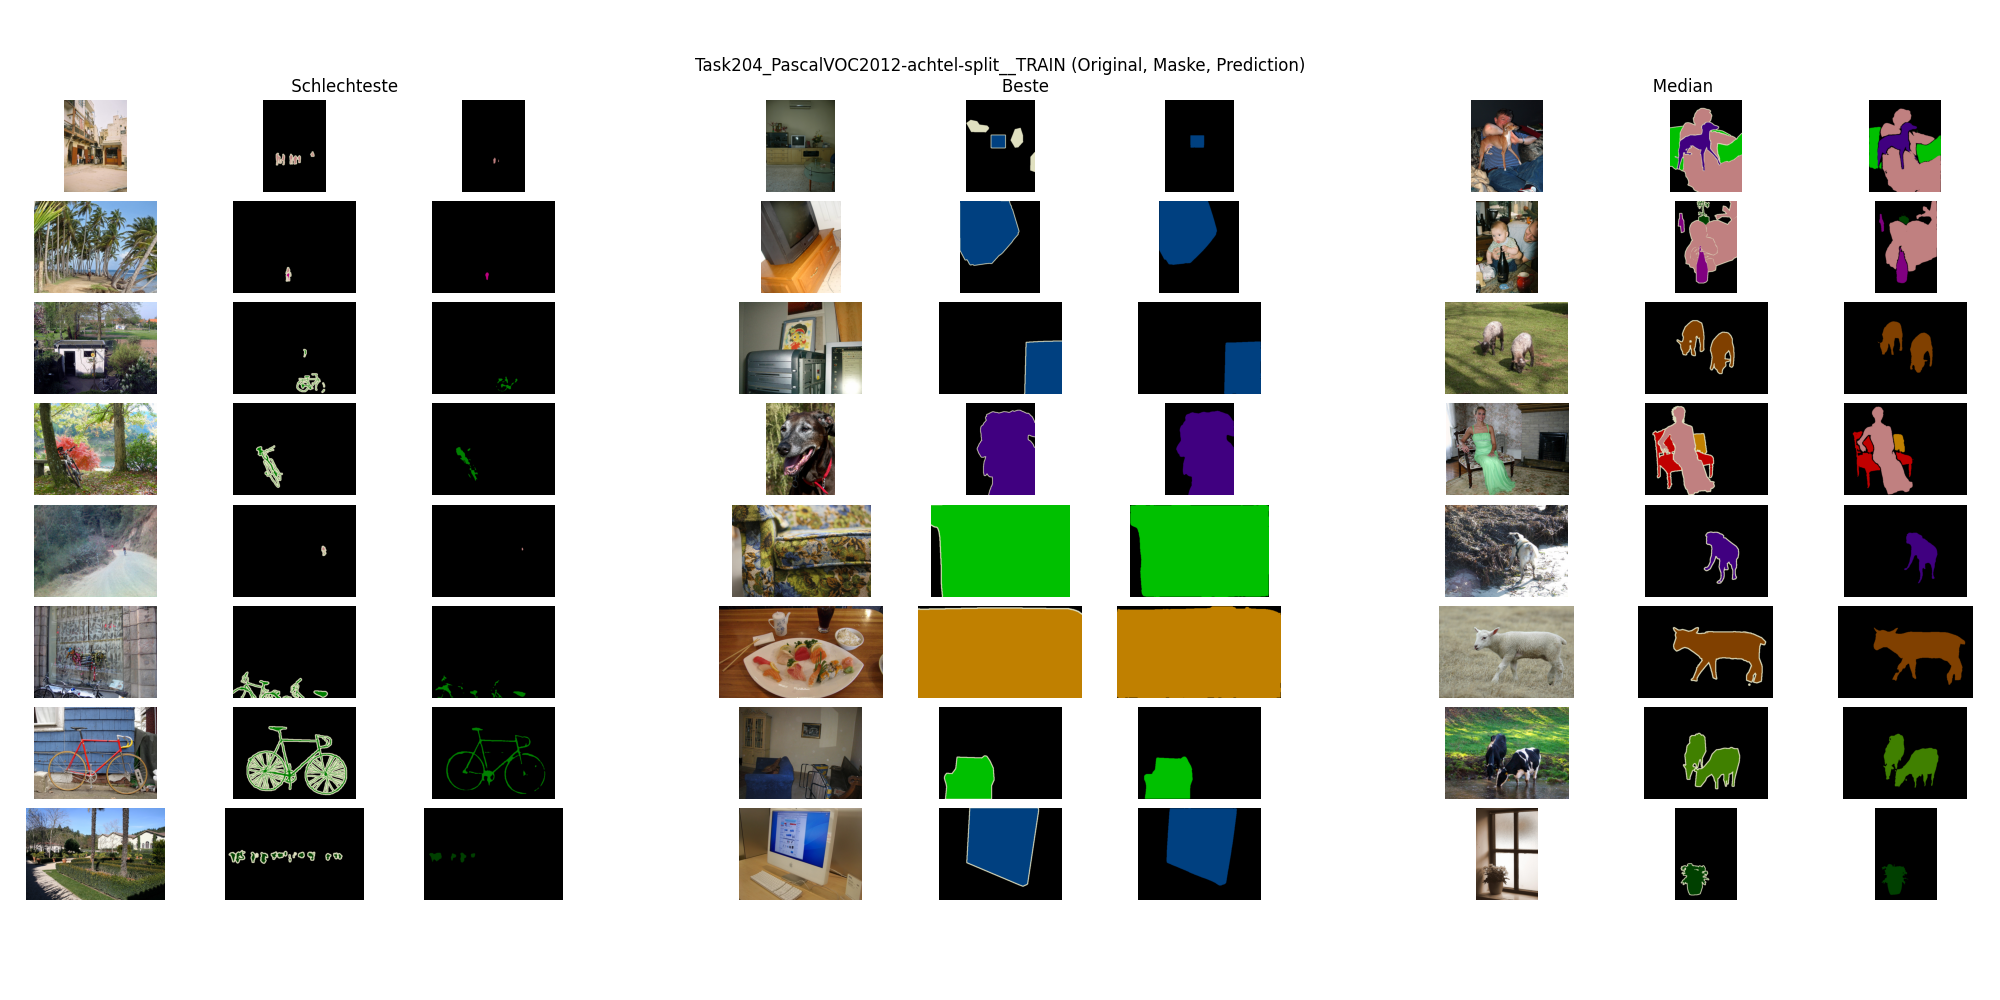
\includegraphics[height=0.35\textheight, width=\textwidth]{Pictures/nnUnet/Praxis/Task204-Pascal-VOC12-achtel-testsplit/Vis-Train.png}
\caption{Visualisierung des Testsplits auf dem PascalVOC 12 \cite{PascalVOCDatensatz} Datensatz (links: schlechteste Ergebnisse, mitte: beste Ergebnisse, rechts: Ergebnisse im Median; jeweils Original, Ground-Truth und Prediction)}
\label{pic:Vis-Test_204}
\end{figure}

\subsection{Retina 3D-Datensatz}
\begin{figure}[H]
\begin{minipage}{.5\textwidth}
\begin{subfigure}{\textwidth}
\includesvg[width=\textwidth]{Pictures/nnUnet/Praxis/Task108-Retina3D/Haeufigkeitsverteilung-108-Train}
\caption{Trainsplit}
\label{pic:Haeuf-Train_108}
\end{subfigure}
\end{minipage}
\begin{minipage}{.5\textwidth}
\begin{subfigure}{\textwidth}
\includesvg[width=\textwidth]{Pictures/nnUnet/Praxis/Task108-Retina3D/Haeufigkeitsverteilung-108-Test}
\caption{Testsplit}
\label{pic:Haeuf-Test_108}
\end{subfigure}
\end{minipage}
\caption{Anteil von Objekt (Ader) je Sample mit Durchschnitt je Split $\approx$ 0.55\%}
\label{pic:Haeuf_108}
\end{figure}
Abschließend haben wir, da wir auf dem anderen 3D-Datensatz mit CT-Aufnahmen keine besonders guten Ergebnisse erzielen konnten, einen weiteren 3D-Datensatz mit Retinae zur Verfügung gestellt bekommen \cite{retina3dDatensatz}. Er besteht aus 21 Samples von 3D-Scans der Retina mit Segmentierungen. Diese Samples liegen sowohl in ihrer ursprünglichen, gekrümmten Form vor als auch in einer geplätteten Form, die die Krümmung der Netzhaut heraus rechnet. Wir haben uns auf die gekrümmte Version beschränkt.\\\\
Wir haben wieder die zur Verfügung gestellten .mat Dateien in Niftis konvertiert \cite{autoMLGithub} und das Training gestartet. Der Objektanteil in dem Datensatz ist sowohl im Train- als auch im Testsplit im Vergleich zu dem 2D-Retina Datensatz \cite{retina2d} um ein Vielfaches geringer, jedoch deutlich höher als bei dem CT-Datensatz (s. Abbildung \ref{pic:Haeuf_108})
\begin{figure}[H]
\begin{minipage}{.5\textwidth}
\begin{subfigure}{\textwidth}
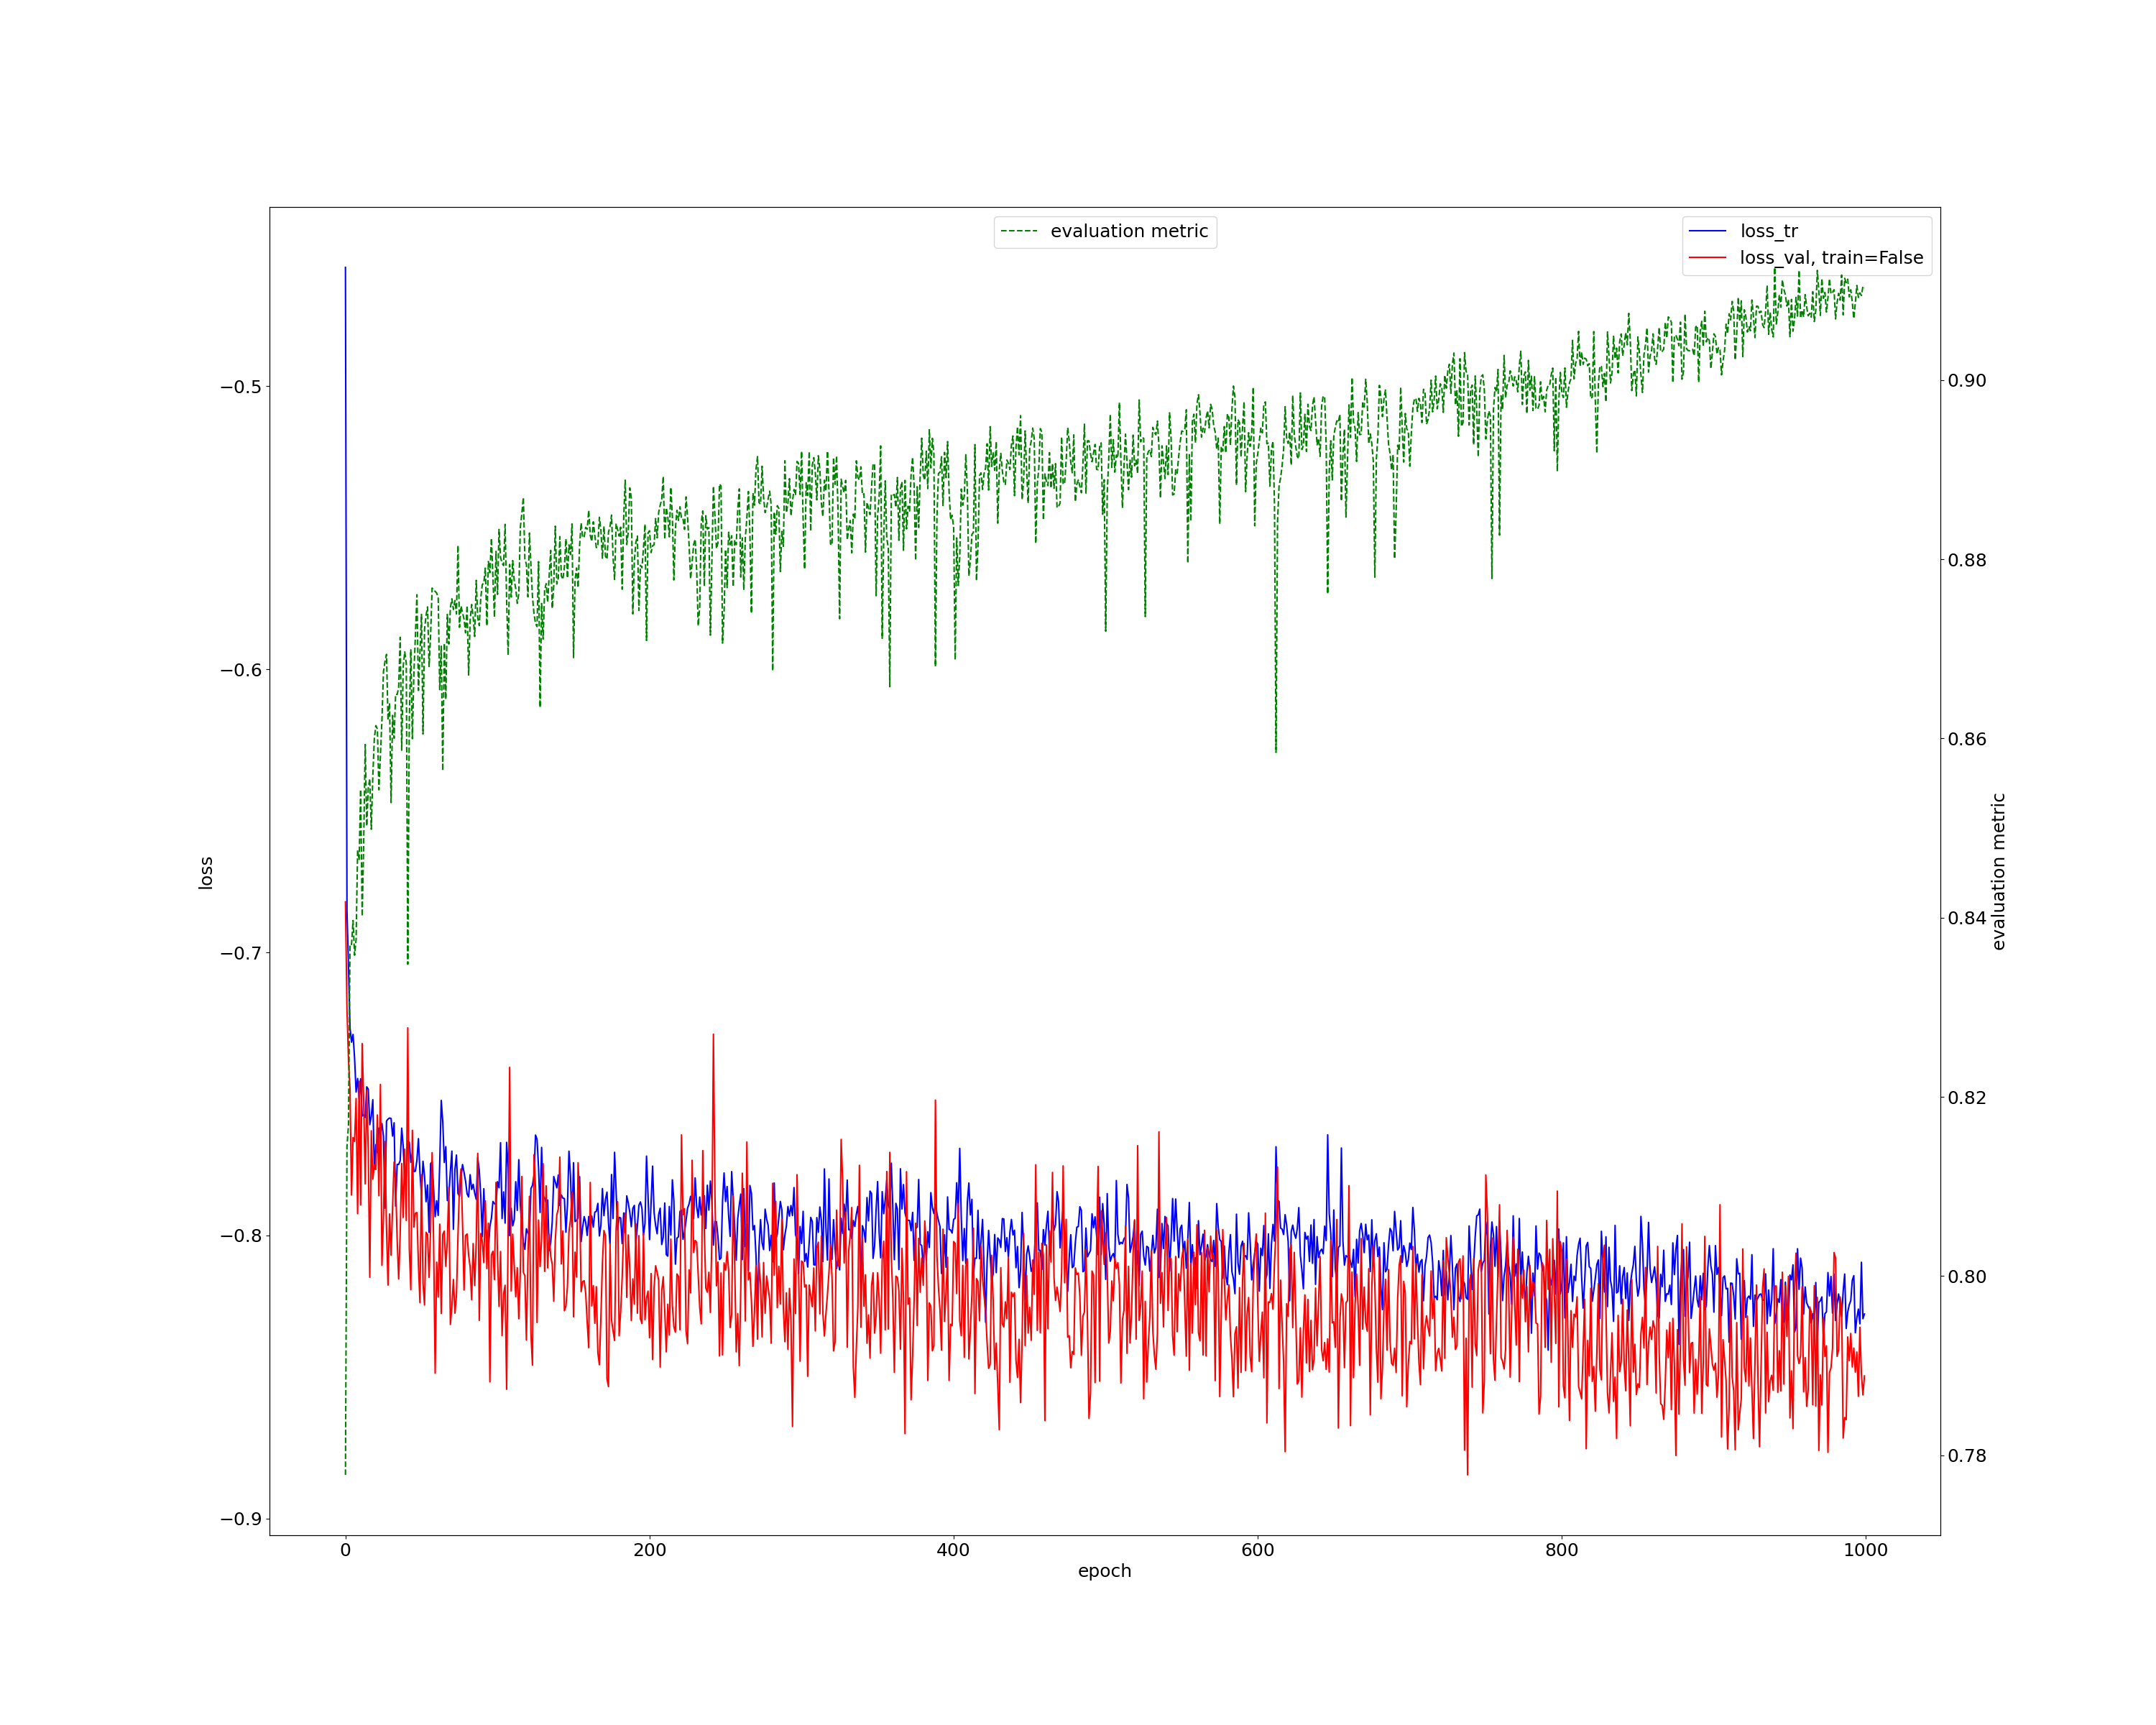
\includegraphics[width=\textwidth]{Pictures/nnUnet/Praxis/Task108-Retina3D/progress_108-Retina3D_3dFullres.png}
\caption{3D\_fullres Netz-Variante}
\label{pic:Prog_108-3dfullres}
\end{subfigure}
\end{minipage}
\begin{minipage}{.5\textwidth}
\begin{subfigure}{\textwidth}
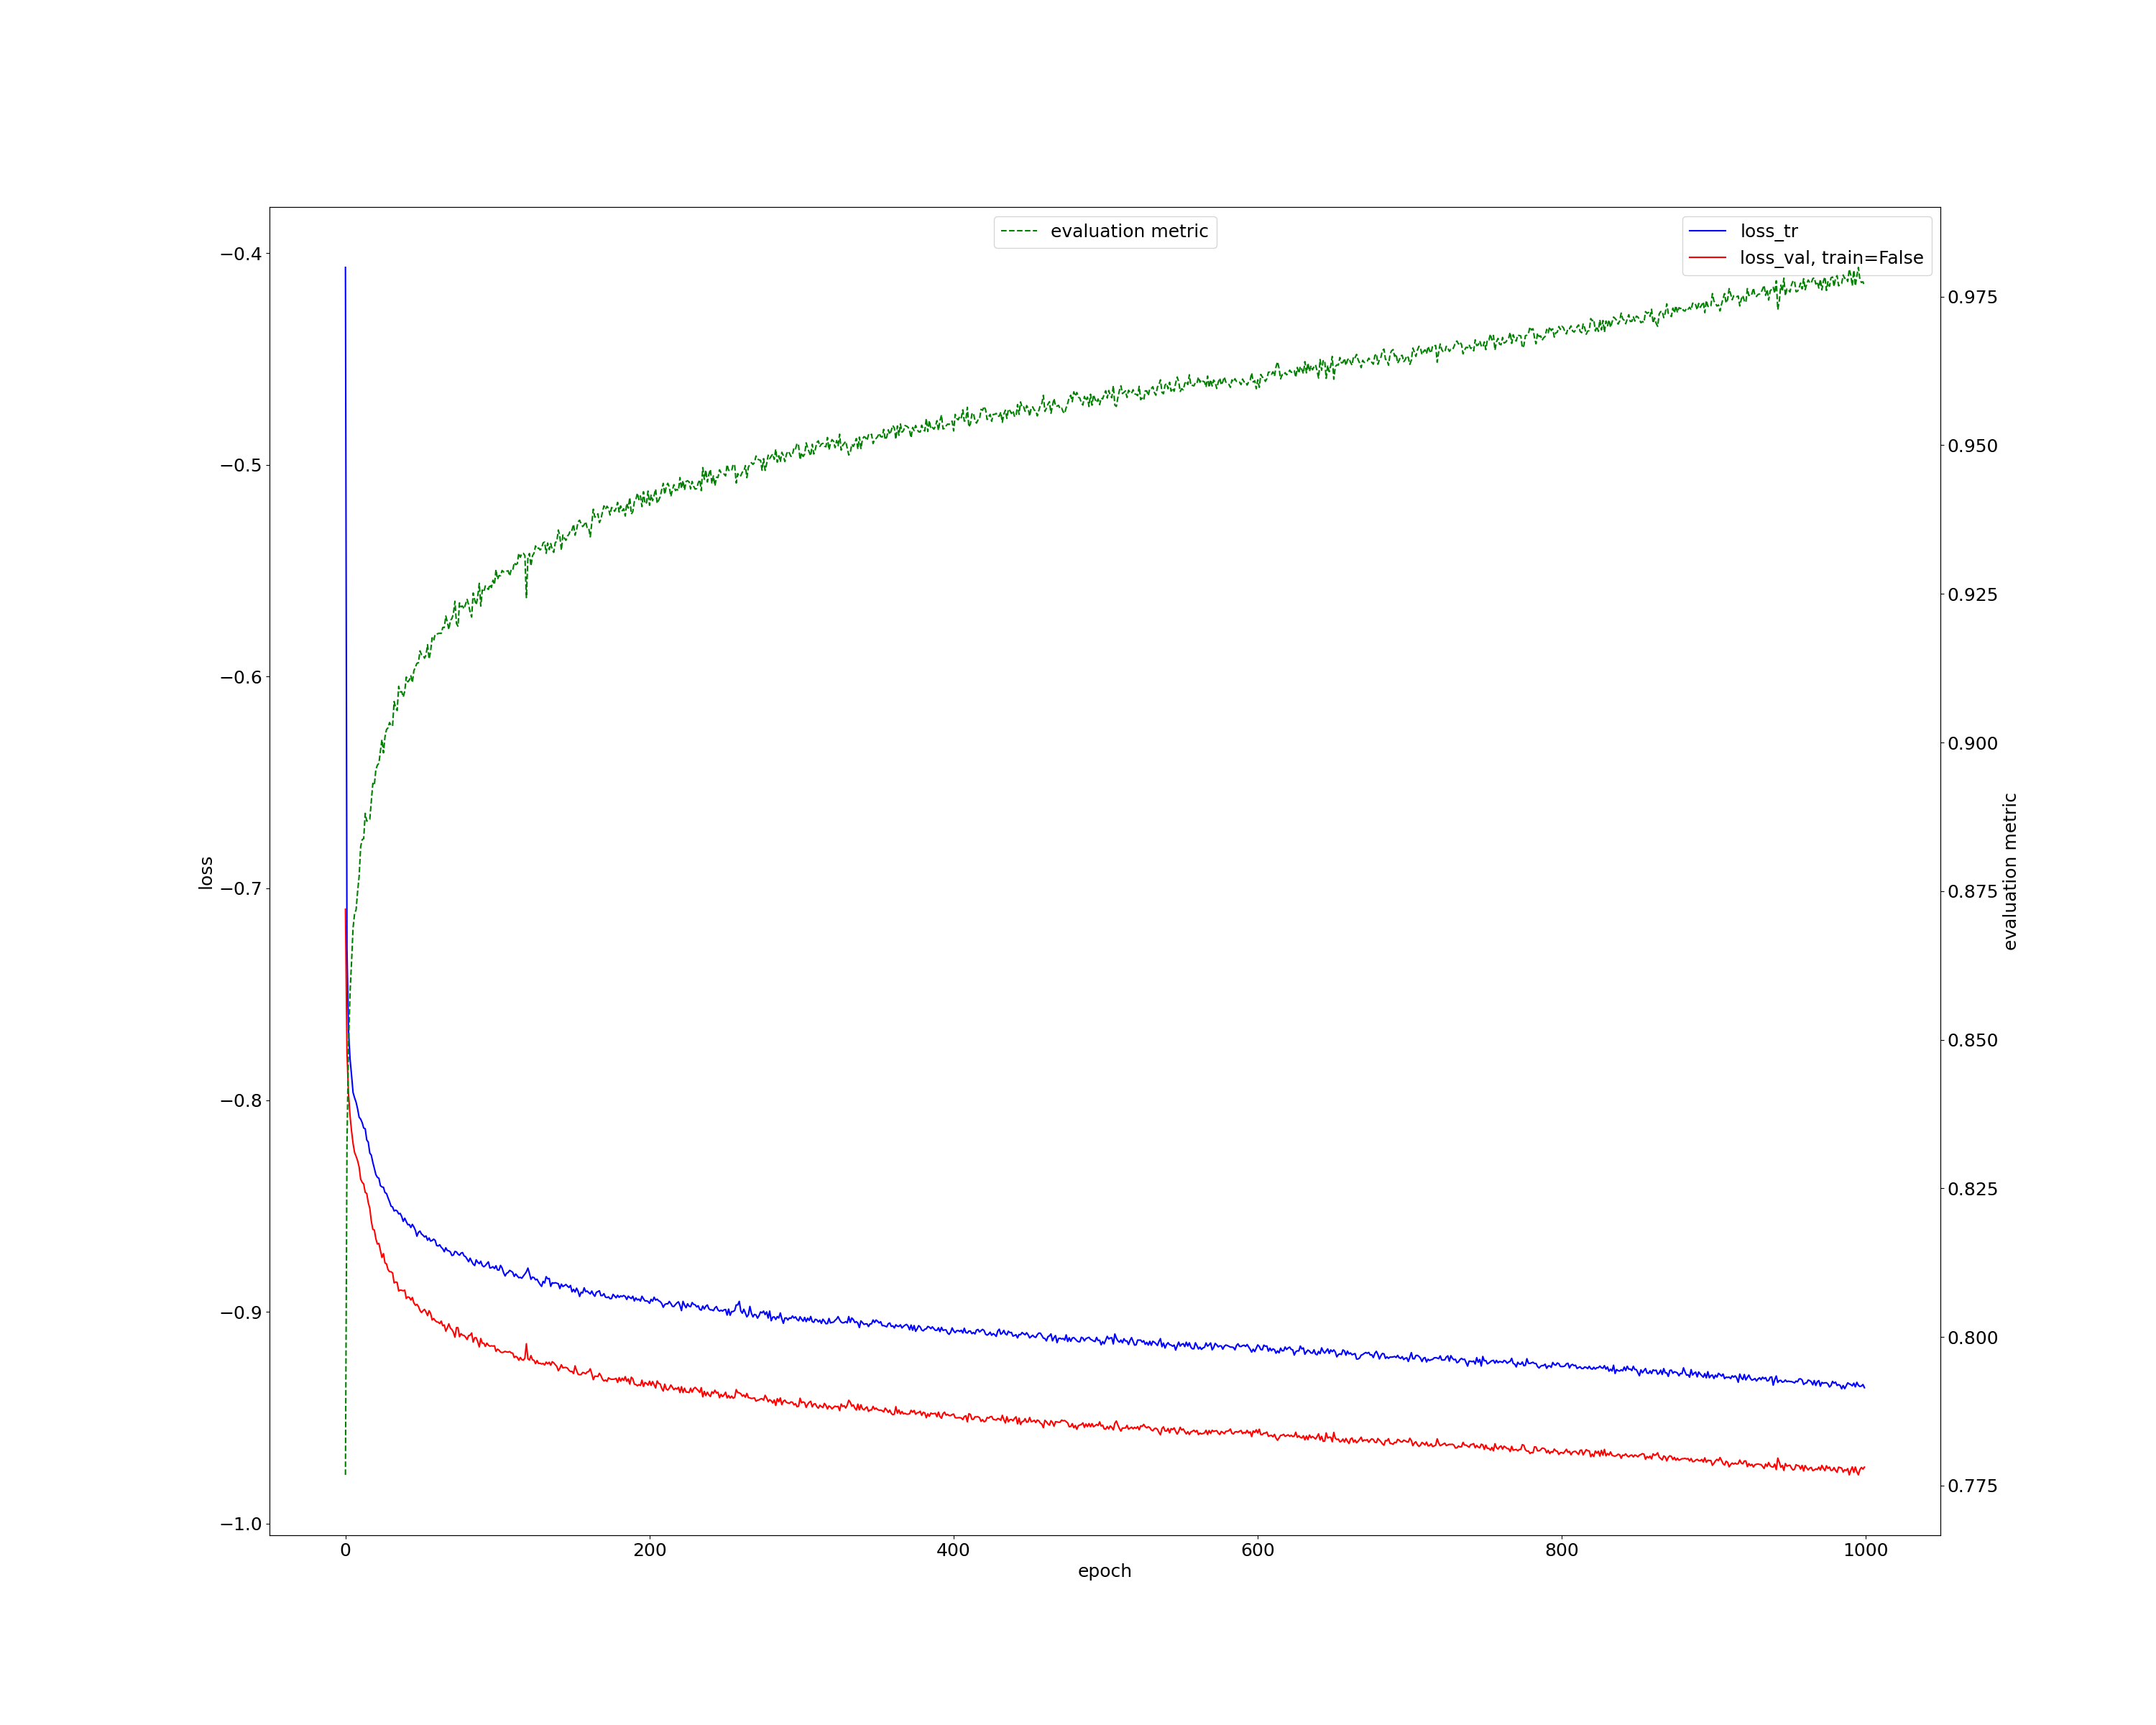
\includegraphics[width=\textwidth]{Pictures/nnUnet/Praxis/Task108-Retina3D/progress_108-Retina3D_2DNet.png}
\caption{2D Netz-Variante}
\label{pic:Prog_108-2d}
\end{subfigure}
\end{minipage}
\caption{Progress-Graphen für Retina 3D in den Netzvarianten 3D\_fullres und 2D.}
\label{pic:Prog_108}
\end{figure}



\begin{figure}[H]
\begin{minipage}{.3\textwidth}
\begin{subfigure}{\textwidth}
\includesvg[width=\textwidth]{Pictures/nnUnet/Praxis/Task108-Retina3D/Scatterplot-Dice-108-Retina_3d_fullres}
\caption{3D\_fullres Netz-Variante}
\label{pic:Dice_108-3dfullres}
\end{subfigure}
\end{minipage}
\begin{minipage}{.3\textwidth}
\begin{subfigure}{\textwidth}
\includesvg[width=\textwidth]{Pictures/nnUnet/Praxis/Task108-Retina3D/Scatterplot-Dice-108-Retina_2d}
\caption{2D Netz-Variante}
\label{pic:Dice_108-2d}
\end{subfigure}
\end{minipage}
\begin{minipage}{.3\textwidth}
\begin{subfigure}{\textwidth}
\includesvg[width=\textwidth]{Pictures/nnUnet/Praxis/Task108-Retina3D/Scatterplot-Dice-108-Retina_ensemble}
\caption{Ensemble von \ref{pic:Dice_108-2d} und \ref{pic:Dice_108-3dfullres}}
\label{pic:Dice_108-ensemble}
\end{subfigure}
\end{minipage}
\caption{Scatterplot mit Dice-Koeffizienten je Sample für Retina 3D in den Netzvarianten 3D\_fullres, 2D und ihrem Ensemble}
\label{pic:Dice_108}
\end{figure}


Es fällt auf, dass insgesamt die 2D Netz-Variante auf dem Trainsplit am besten abschneidet, während die 3D\_fullres Netz-Variante auf dem Testsplit am besten abschneidet. Das Ensemble aus den beiden Varianten ist im Trainsplit schlechter als als 2D, aber besser als 3D\_fullres und auf dem Testsplit besser als 2D aber schlechter als 3D\_fullres (s. Abbildung \ref{pic:Dice_108}).\\\\
Anhand von Abbildung \ref{pic:Vis_108} sieht man beispielhaft, dass das 3D\_fullres Netz im Testsplit feine Adern ein bisschen besser erkennt als das 2D Netz. Insgesamt sieht man bei beiden Netz-Varianten und dem Ensemble keine groben Fehler.

\begin{figure}[H]
\begin{minipage}{.3\textwidth}
\begin{subfigure}{\textwidth}
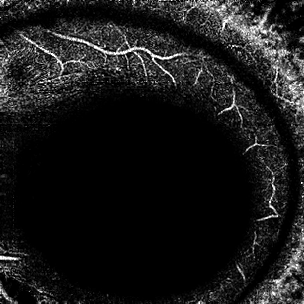
\includegraphics[width=\textwidth]{Pictures/nnUnet/Praxis/Task108-Retina3D/vis/orig_008_0000-66.png}
\caption{Original}
\end{subfigure}
\end{minipage}
\begin{minipage}{.3\textwidth}
\begin{subfigure}{\textwidth}
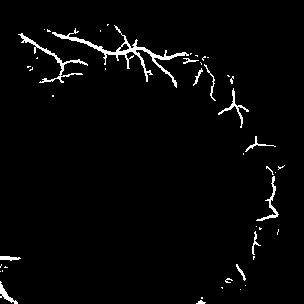
\includegraphics[width=\textwidth]{Pictures/nnUnet/Praxis/Task108-Retina3D/vis/gt_008-66.png}
\caption{Ground-Truth}
\end{subfigure}
\end{minipage}
\begin{minipage}{.3\textwidth}
\begin{subfigure}{\textwidth}
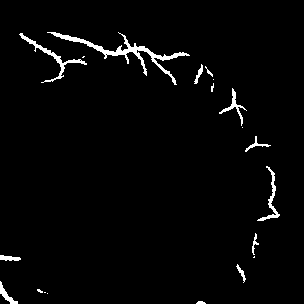
\includegraphics[width=\textwidth]{Pictures/nnUnet/Praxis/Task108-Retina3D/vis/pred2d_008-66.png}
\caption{Prediction (2D)}
\end{subfigure}
\end{minipage}
\begin{minipage}{.3\textwidth}
\begin{subfigure}{\textwidth}
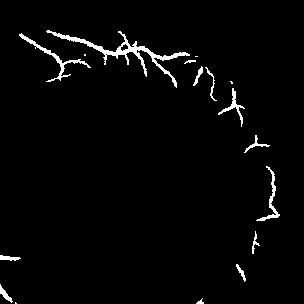
\includegraphics[width=\textwidth]{Pictures/nnUnet/Praxis/Task108-Retina3D/vis/pred3d_008-66.png}
\caption{Prediction (3D\_fullres)}
\end{subfigure}
\end{minipage}
\begin{minipage}{.3\textwidth}
\begin{subfigure}{\textwidth}
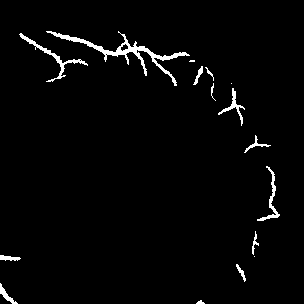
\includegraphics[width=\textwidth]{Pictures/nnUnet/Praxis/Task108-Retina3D/vis/ens_008-66.png}
\caption{Prediction (Ensemble)}
\end{subfigure}
\end{minipage}
\caption{Visualisierung eines zufällig ausgewählten Samples aus dem Testsplit (Nummer 008) und dessen Prediction}
\label{pic:Vis_108}
\end{figure}






\section{Fazit}

Für die Installation des Frameworks von nnU-Net ist eine vollständige und gut funktionierende Installationsanleitung vorhanden, welche uns den Einstieg und die Installation des Frameworks sehr erleichtert hat. Die Entwickler von nnU-Net liefern außerdem eine gute Einführung in die Arbeit mit dem Framework, in welcher sie erklären welches Dateiformat vom Framework erwartet wird und in welchen Ordnerstrukturen welche Dateien eingefügt werden müssen. Sie liefern außerdem guten Support bezüglich der Wahl wichtiger Parameter. Auch positiv aufgefallen sind uns die schnellen Antworten der Entwickler auf Fragen, welche in den Github-Issues gestellt wurden. Auch wird das Framework auf Github ständig weiterentwickelt und es gibt schnelle Bug-Fixes. 

Der Code von nnU-Net ist übersichtlich gestaltet und gut kommentiert, wodurch man rasch einen guten Überblick darüber bekommt, was wo passiert. Daher lässt er sich auch gut nachvollziehen und so auch gut damit arbeiten, da eindeutig klar ist, welcher Code für was zuständig ist. Außerdem ist der Code darauf ausgelegt, allgemein und für verschiedene Benutzer zu funktionieren, sodass zum Beispiel keine Dateipfade angepasst werden müssen.  
Das Framework gibt gute und sinnvolle Fehlermeldungen zurück. Der Code arbeitete für uns absolut zuverlässig und tat genau das was er sollte. 

Die Einarbeitung in das Framework war daher sehr leicht umsetzbar und die Arbeit gestaltet sich sehr nutzerfreundlich und effizient. 

In den zwei Papern von nnU-Net erhält man sowohl einen guten Überblick über die Grundidee und die Ziele des Papers, als auch gut verständliche Informationen über die Details der Idee und der Implementierung. Auf diese Art sind die verarbeiteten Ideen und Überlegungen gut verständlich und eindeutig. 

Bezüglich der Performance hält das Framework, was es auf den Datensätzen verspricht und konnte bei uns die gleichen guten Ergebnisse erzielen wie im Paper angegeben. Das Framework arbeitet sehr gut und zuverlässig auf medizinischen Bildern, von denen bei uns alle sehr ähnliche Muster innerhalb des jeweiligen Datensatzes hatten. Die Ergebnisse auf diesen Datensätzen waren gut bis sehr gut und blieben auch dann gut, wenn das Verhältnis aus Hintergrund und Maske nicht gut war, so zum Beispiel auf dem Retina-3D Datensatz \cite{retina3dDatensatz}. 
Bei einem sehr schlechten Verhältnis zwischen Maske und Hintergrund, wie zum Beispiel in unserem CT-Datensatz \cite{ctDatensatz} zu den Verkalkungen in Blutgefäßen, werden die Ergebnisse dann aber auch bei diesem Framework merklich schlechter, bleiben aber aus unserer Sicht in Anbetracht der erschwerten Umstände akzeptabel, wenn auch deutlich verbesserungswürdig. 
Die Ergebnisse des Frameworks auf mehreren Klassen sind jedoch nicht so gut. Auffällig ist hier, dass der Datensatz PascalVOC12 \cite{PascalVOCDatensatz}, welchen wir als Test für mehrere Klassen verwendet haben, deutlich unregelmäßiger in sich selbst war, als die medizinischen Datensätze. Unseren Ergebnissen zu Folge kommt das Framework entweder mit dieser Unregelmäßigkeit, oder mit den mehreren Klassen nicht so gut klar. Wie gut das Framework auf medizinischen, regelmäßigen Datensätzen mit mehreren Klassen klarkommt, könnte man in der Zukunft noch versuchen herauszufinden. 

Insgesamt können wir feststellen, dass das Framework im Bereich der Segmentierung medizinischer Datensätze gute Arbeit macht. Aufgrund der positiven und immer aktuellen Aktivität der Entwickler auf Github, der großen Nutzerfreundlichkeit des Frameworks und der guten Ergebnisse erscheint eine Nutzung und Arbeit mit dem Framework für uns als sehr sinnvoll. 
Wegen der guten Verständlichkeit des Codes, der Grundidee und der Nutzung der verwendeten Konzepte eignet sich das Netz durchaus auch zur Weiterarbeit und Weiterentwicklung. Aufgrund des guten Verständnisses und der guten Übersicht über verwendete Ideen und Methoden fällt es leicht sich über mögliche Anpassungen Gedanken zu machen. So zum Beispiel über eine mögliche andere Kombination von Verlustfunktionen, wenn man nicht mit medizinischen Datensätzen arbeiten möchte und die Empfindlichkeit auf Hintergrundklassen anpassen möchte. 






